% Vorlage für eine Bachelorarbeit
% Siehe auch LaTeX-Kurs von Mathematik-Online
% www.mathematik-online.org/kurse
% Anpassungen für die Fakultät für Mathematik
% am KIT durch Klaus Spitzmüller und Roland Schnaubelt im Dezember 2011

\documentclass[11pt,a4paper,titlepage]{scrartcl}
% scrartcl ist eine abgeleitete Artikel-Klasse im Koma-Skript
% zur Kontrolle des Umbruchs Klassenoption draft verwenden

\usepackage{array}
% die folgenden Packete erlauben den Gebrauch von Umlauten und ß
% in der Latex Datei
\usepackage[utf8]{inputenc}
% \usepackage[latin1]{inputenc} %  Alternativ unter Windows
\usepackage[T1]{fontenc}
\usepackage[ngerman]{babel}
\usepackage[babel,german=quotes]{csquotes}
\usepackage[pdftex]{graphicx}
\usepackage{latexsym}
\usepackage{amsmath,amssymb,amsthm}
\usepackage[style=alphabetic,backend=biber]{biblatex}
\usepackage{pdflscape}
\usepackage{colortbl}
\usepackage{color}
\usepackage{listings}
\usepackage[hidelinks]{hyperref}
\usepackage[framemethod=tikz]{mdframed}
\usepackage{chngcntr}
\usepackage{caption}
\usepackage{pdflscape}

\definecolor{lightgray}{rgb}{.9,.9,.9}
\definecolor{darkgray}{rgb}{.4,.4,.4}
\definecolor{purple}{rgb}{0.65, 0.12, 0.82}
\definecolor{darkviolet}{rgb}{0.5,0,0.4} 
\definecolor{darkgreen}{rgb}{0,0.4,0.2} 
\definecolor{darkblue}{rgb}{0.1,0.1,0.9} 
\definecolor{darkgrey}{rgb}{0.5,0.5,0.5} 
\definecolor{lightblue}{rgb}{0.4,0.4,1} 

\lstdefinelanguage{JavaScript}{
	keywords={typeof, private, let, new, true, false, catch, function, return, null, catch, switch, var, if, in, while, do, else, case, break},
	keywordstyle=\color{purple}\bfseries,
	ndkeywords={class, export, boolean, throw, implements, import, this},
	ndkeywordstyle=\color{darkgray}\bfseries,
	identifierstyle=\color{black},
	sensitive=false,
	comment=[l]{//},
	morecomment=[s]{/*}{*/},
	commentstyle=\color{purple}\ttfamily,
	stringstyle=\color{darkblue}\ttfamily,
	morestring=[b]',
	morestring=[b]"
}

\lstset{ 
	language=Java, 
	basicstyle=\footnotesize\ttfamily,
	keywordstyle=\color{darkviolet}\bfseries, 
	commentstyle=\color{darkgreen}, 
	stringstyle=\color{darkblue}, 
	morecomment=[s][\color{lightblue}]{/**}{*/}, 
	showstringspaces=false, 
	showspaces=false,
	extendedchars=true,
	tabsize=2,
	captionpos=b,
	showtabs=false,
	breaklines=true
	%numbers=left 
} 



\bibliography{bib/Quellen}

\usepackage[footskip=1.5cm, left=2.5cm, right=2.5cm, top=2.5cm, bottom=3.5cm]{geometry}

% Definieren von versch. Farben für Tabellenzellen
\definecolor{grey}{rgb}{0.85,0.85,0.85}
\definecolor{lightgrey}{rgb}{0.95,0.95,0.95}

% Abstand obere Blattkante zur Kopfzeile ist 2.54cm - 15mm
\setlength{\topmargin}{-15mm}
\usepackage[onehalfspacing]{setspace}

% Umgebungen für Definitionen, Sätze, usw.
% Es werden Sätze, Definitionen etc innerhalb einer Section mit
% 1.1, 1.2 etc durchnummeriert, ebenso die Gleichungen mit (1.1), (1.2) ..

\newtheorem{Satz}{Satz}[section]
\newtheorem{Definition}[Satz]{Definition}     
\newtheorem{Lemma}[Satz]{Lemma}	
                  
\numberwithin{equation}{section} 
\counterwithin{figure}{section}
\counterwithin{table}{section}

% einige Abkuerzungen
\newcommand{\C}{\mathbb{C}} % komplexe
\newcommand{\K}{\mathbb{K}} % komplexe
\newcommand{\R}{\mathbb{R}} % reelle
\newcommand{\Q}{\mathbb{Q}} % rationale
\newcommand{\Z}{\mathbb{Z}} % ganze
\newcommand{\N}{\mathbb{N}} % natuerliche

\title{Bachelorarbeit}
\author{Andre Weinkötz (14985714)}
\date{15. Februar 2018}


\begin{document}
  % Keine Seitenzahlen im Vorspann
  \pagestyle{empty}
  \renewcommand{\thelstlisting}{\arabic{section}.\arabic{lstlisting}}
 \counterwithin{lstlisting}{section}
  % Titelblatt der Arbeit
\begin{titlepage}

\begin{center}
	\includegraphics[scale=0.20]{img/hm-logo.eps}
\end{center}
 \bigskip

 \begin{center} \large 
    
    Bachelorarbeit im Studiengang B.Sc. Wirtschaftsinformatik
    \vspace*{2cm}
\end{center}
\begin{doublespace}
	{\huge Realisierung einer bidirektionalen Chat-Anwendung auf Basis von HTML5 WebSockets mit Java und Angular 4 zum Einsatz im seminaristischen Kontext}\\
\vspace{1.5cm}

	{\huge \noindent Implementation of a bidirectional chat application utilizing HTML5 WebSockets in Java and Angular 4 for use in a seminaristic context}
\end{doublespace}

    
    \vspace*{2.0cm}
 \begin{center}
    Andre Weinkötz \bigskip
    
    

    15. Februar 2018
    \vspace*{2.5cm}
    
    

    Fakultät für Informatik und Mathematik \\
	Hochschule München\bigskip
	
	Betreuer: Prof. Dr. Mandl 
	
	
  \end{center}
\end{titlepage}
\newpage
\vspace*{9cm}
\begin{quote}
\onehalfspacing{{\Large \textit{People keep asking me what I think of it now that it's done. }\\\textit{Hence my protest: The Web is not done!}\\}}
\medskip
	Tim Berners-Lee
\end{quote}
\newpage
\section*{Abstract}
\addcontentsline{toc}{section}{Abstract}

\newpage
  % Inhaltsverzeichnis
 \tableofcontents

\newpage

%\newpage
  % Ab sofort Seitenzahlen in der Kopfzeile anzeigen
  \pagestyle{headings}

\section{Einleitung}\label{sec:Einleitung}
Der Austausch von Informationen ist für die heutige Gesellschaft von fundamentaler Bedeutung. Deren digitale Repräsentation variierte je nach verwendetem System bis zur Entwicklung des World Wide Web (WWW) durch Tim Berners-Lee im Jahr 1989. Geleitet von seinem Grundgedanken eines möglichst einfachen, lizenzfreien und verteilten Systems entwickelte er das Hypertext Transfer Protocol (HTTP), die Hypertext Markup Language (HTML) und die Uniform Resource Identifier (URI). Diese Simplizität trägt noch heute zur Popularität des WWW bei. Doch die Anforderungen an Webanwendungen haben sich in den vergangenen Jahren stark verändert. Mobile Geräte wie Smartphones oder Tablets ersetzen stationäre Systeme, Webanwendungen sollen zur Kollaboration eingesetzt werden und Buchungssysteme oder Finanzanwendungen verlangen die Bearbeitung tausender Anfragen mit minimaler Verzögerung. HTTP bietet hier keine zufriedenstellende Lösung. Um den Anforderungen an moderne Webanwendungen gerecht zu werden, spezifizierten das World Wide Web Consortium (W3C) und die Internet Engineering Taskforce (IETF) das WebSocket-Protokoll mit zugehöriger JavaScript-API. Dabei machten die Entwickler es sich zur Aufgabe, einen Mechanismus zu standardisieren, der es browserbasierten Anwendungen ermöglicht bidirektional zu kommunizieren ohne dabei mehrere HTTP Verbindungen zu öffnen \autocite{fette_websocket_2011}.\\

\noindent HTML5 WebSockets sollen die Vorteile webbasierter Architekturen mit den Eigenschaften des verbindungsorientierten Protokolls TCP kombinieren. Dadurch können Webanwendungen mit nur wenigen Verwaltungsdaten Informationen gleichzeitig senden und empfangen. Eine hohe Kompabilität zu bestehenden Web-Infrastrukturen und Sicherheitssystemen ist gewährleistet, da das WebSocket-Protokoll von aktuellen Webservern bereitgestellt werden kann. Das Ziel dieser Arbeit ist die Migration der Kommunikationsstrukturen einer bestehenden Anwendung auf HTML5 WebSockets, um von diesen Vorteilen profitieren zu können. Bei der Anwendung handelt es sich um ein Chatsystem, welches im Rahmen der Lehrveranstaltung \glqq Datenkommunikation\grqq{} im dritten Semester des Studiengangs B.Sc. Wirtschaftsinformatik an der Hochschule München eingesetzt wird. Die zu entwickelnde Anwendung soll zur Ergänzung des Lehrmittelportfolios in passenden Lehrveranstaltungen eingesetzt werden können. Die Voraussetzung für eine fachgerechte Umsetzung der Anforderungen ist ein fundiertes Verständnis von den Funktionsweisen der WebSockets sowie deren Implementierung in verschiedenen Programmiersprachen.\\

\noindent Der Aufbau dieser Arbeit gliedert sich in sechs Kapitel. In Kapitel 2 wird das WebSocket-Protokoll anhand seiner Spezifikation detailliert erläutert. Kapitel 3 behandelt die zugehörige WebSocket-API und beschreibt deren Implementierung in der Programmiersprache Java. In Kapitel 4 wird die bestehende Chatanwendung analysiert, die Architektur des neuen WebSocket-Chats entworfen und anschließend implementiert. Diese Implementierung wird in Kapitel 5 evaluiert, indem die Messergebnisse der Leistungstest beider Anwendungen verglichen werden. Kapitel 6 schließt mit einem Fazit und gibt einen Ausblick auf die zukünftige Entwicklung und offene Aspekte.

\newpage
\section{Das WebSocket Protokoll}\label{sec:WebSocketProtokoll}
Die Arbeit an der Spezifikation des WebSocket-Protokolls begann bereits 2009, als es von Google in Zusammenarbeit mit Apple, Microsoft und Mozilla im Rahmen ihrer Kooperation WHATWG\footnote{Web Hypertext Application Technology Working Group unter: www.whatwg.org} der Internet Engineering Task Force (IETF) vorgeschlagen wurde. Bis Mai 2010 wurden noch zahlreiche Verbesserungen hinzugefügt, bis es schließlich in Version 76 \autocite{hickson_websocket_2010} im August 2010 an die \textit{BiDirectional or Server-Initiated HTTP} (HyBi) Task Force der IETF zur Weiterentwicklung übergeben wurde \autocite{fette_websocket_2010}. Neben vielen anderen Fortschritten wurde das Protkoll um die Möglichkeit erweitert binäre Dateien auszutauschen, sowie Sicherheitslücken geschlossen, die in Verbindung mit Proxy-Servern entstehen konnten. Im Dezember 2010 wurde das WebSocket-Protokoll von der IETF zu dem Request for Comment (RFC) 6455 erklärt \autocite{fette_websocket_2011}. Dieser definiert auf über 70 Seiten neben den Kommunikationsphasen und verschiedenen Frames der WebSockets noch zahlreiche weitere technische Details und Defintionen. In diesem Kapitel sollen die wichtigsten Grundlagen der Protokollspezifikation dargelegt werden.\\
\begin{figure}[ht] \label{fig:wsOSI}
\begin{center}
	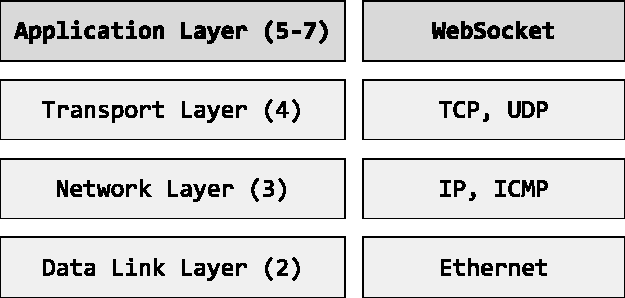
\includegraphics[scale=1]{img/osi.pdf}
	\caption{WebSocket-Protokoll im ISO/OSI-Modell}
\end{center}
\end{figure}

\noindent Die Aufgabe des WebSocket-Protokolls ist die bidirektionale Kommunikation zwischen einer (Web-)Anwendung und einem WebSocket-Server. Dabei folgt das Protokoll dem Prinzip des minimalen \textit{Framings} \autocite[9-10]{fette_websocket_2011}. Das bedeutet, dass Zusatzinformation zur Übermittlung von Nachrichten, wie z.B. Protokoll-Header, möglichst gering zu halten sind. Das Konzept sieht vor, dass das WebSocket-Protokoll direkt als Schicht auf das \textit{Transmission Control Protocol} (TCP) aufsetzt und es neben HTTP in einer bereits bestehenden Infrastruktur eingesetzt werden kann. Dabei wird das Sicherheitsmodell der Same-Origin-Policy aus RFC 6454 sowie ein Adressierungs- und Bezeichnungsmechanismus hinzugefügt, durch welchen die Unterstützung mehrerer Dienste auf einem Port und verschiedener Hostnamen unter einer IP-Adresse sichergestellt wird. Des weiteren soll das aufgesetzte Framing den Paketierungsmechanismus des \textit{Internet Protocols} (IP) imitieren, ohne die Länge eines Frames zu beschränken. Außerdem wird ein zusätzlicher \textit{Closing-Handshake} definiert, der auch bei der Verwendung von Proxy-Servern und anderen \textit{Vermittlern}, wie z.B. Firewalls, zwischen den beiden Endpunkten durchgeführt werden kann. Obwohl das WebSocket-Protokoll die für HTTP(S) vorgesehenen Ports 80 und 443 verwendet, verbindet die beiden Protokolle lediglich der \textit{HTTP Upgrade}-Mechanismus. Dieser kommt zum Einsatz, wenn eine WebSocket-Verbindungsanfrage von einem HTTP-Server interpretiert wird. Soll die WebSocket-Verbindung verschlüsselt sein, so kann dies durch die Verwendung eines \textit{Transport Layer Security} (TLS) Tunnels erreicht werden.

\subsection{WebSocket-Frames}\label{subsec:wsFrames}
Die Spezifikation eines WebSocket-Frames sieht eine Zweiteilung vor, wie sie bei Protokollnachrichten üblicherweise vorgenommen wird. Ein WebSocket-Frame besteht demnach aus einem Header Bereich der Kontrolldaten enthält, sowie dem Payload, welcher die Nutzdaten beinhaltet.\vspace{2mm}
\begin{figure}[ht] \label{fig:wsFrame}
	\begin{center}
		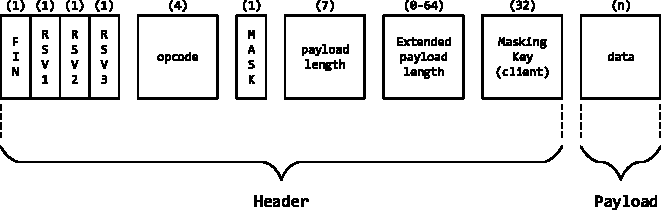
\includegraphics[scale=1.25]{img/frame.pdf}
		\caption{Vereinfachte Darstellung eines WebSocket Frames}
	\end{center}
\end{figure}
Anhand des Aufbaus ist leicht erkennbar, dass die Kommunikation über WebSockets mit deutlich geringeren Paketgrößen arbeiten kann als HTTP. Eine Nachricht mit einfacher Längenangabe, die von Server zu Client geschickt wird, erzeugt durch ihren Header lediglich einen Overhead von zwei Byte. Da WebSocket-Frames auf umgekehrtem Weg zusätzlich noch maskiert werden müssen, entspricht die minimale Länge eines clientseitigen Frames sechs Byte. Im Vergleich dazu beträgt der Overhead bei einer einfachen GET-Anfrage über HTTP/1.1 beim Aufruf des Hosts unter cs.hm.edu 35 Byte. Die Angabe des Hostnamens in HTTP/1.1 ist obligatorisch und trägt maßgeblich zur Größe des HTTP-Frames bei \autocite[128]{leach_hypertext_1999}. 

\subsubsection{Header-Felder}\label{subsubsec:wsHeader}
Im nachfolgenden Abschnitt werden die Felder sowie deren jeweilige Aufgabe detailliert erläutert:

\begin{description}
	\item[FIN (1 Bit)] Das FIN-Flag gibt an, ob es sich bei dem empfangenen Frame um ein Fragment handelt. Kann der Payload nicht auf einmal übertragen werden, so wird die Übertragung über mehrere Frames gesteuert. Das FIN-Flag aller unvollständigen Fragmente weist den Wert 0 auf, wohingegen das finale Fragment mit einer 1 gekennzeichnet ist. Wenn alle Nutzdaten mit einem einzigen Frame übertragen werden können, so trägt dessen FIN-Flag ebenfalls den Wert 1. Eine Fragmentierung ist in den meisten Fällen nicht erforderlich. Liegen Daten jedoch zum Zeitpunkt des Versendens nicht vollständig vor oder können nicht zwischengespeichert werden, so ermöglicht die Fragmentierung der Nachrichten eine teilweise Übertragung. 
	\item[RSV1, RSV2, RSV3 (jeweils 1 Bit)] Diese Flags sind für zukünftige Implementierung reserviert und finden aktuell keine standardisierte Anwendung. Die Ausnahme stellt das RSV1-Bit dar, welches verwendet wird um anzuzeigen, ob eine Nachricht komprimiert wurde oder nicht \autocite{internet_assigned_numbers_authority_websocket_2011}. Daher tragen sie meist den Wert 0. Ist eines dieser Flags gesetzt und die empfangende Stelle hat keine Erweiterung, welches das jeweilige Flag interpretieren kann, so muss die WebSocket-Verbindung geschlossen werden \autocite[27]{fette_websocket_2011}. 
	\item[opcode (4 Bit)] Das opcode-Feld enthält die Angabe wie der Payload zu interpretieren ist. Neben den sogenannten Datenframes bzw. Non-Control-Frames, welche die Art der übertragenen Daten kennzeichnen, sind Control-Frames definiert, die zur Steuerung und Überprüfung der Verbindung verwendet werden. Wird ein unbekannter Opcode empfangen, so wird die WebSocket-Verbindung geschlossen.
	\begin{itemize}
		\item \textbf{0x0} definiert ein Fortsetzungs-Frame
		\item \textbf{0x1} definiert ein Text-Frame
		\item \textbf{0x2} definiert ein Binary-Frame
		\item \textbf{0x3-7} reserviert für weitere Non-Control-Frames
		\item \textbf{0x8} definiert ein Verbindung beenden-Frame
		\item \textbf{0x9} definiert ein Ping-Frame
		\item \textbf{0xA} definiert ein Pong-Frame
		\item \textbf{0xB-F} reserviert für weitere Control-Frames
	\end{itemize}
	\item[MASK (1 Bit)] Aus Sicherheitsgründen müssen alle Frames \textit{maskiert} werden, die von einem Client zu einem Server übertragen werden. Unter Maskierung versteht man dabei die bitweise Abwandlung der Nutzdaten mittels eines Schlüssels (Masking Key), wobei die Länge der Nutzdaten unverändert bleibt. Das MASK-Flag zeigt dabei an, ob der  Payload maskiert ist. Frames, die clientseitig initiert wurden, müssen maskiert sein, wohingegen serverseitige Frames keine Maskierung vornehmen dürfen. Der verwendete Masking-Key muss im gleichnamigen Header-Feld hinterlegt werden.
	\item[payload length (7 Bit)] Hier wird die Länge der Nutzdaten angegeben. Sind diese nicht größer als 125 Bytes, so können sie mit nur einem Frame übertragen werden. Nutzdaten mit einem höheren Speicherplatzbedarf werden je nach Größe mit dem Wert 126 bzw. 127 angegeben. Diese Angaben führen zur Verwendung des Header-Felds \textit{Extended payload length}.
	\item[Extended payload length (16 Bit oder 64 Bit)] Überschreitet die Länge des Payloads 125 Byte, so wird dieses Feld verwendet. Je nach Wert im Header-Feld \textit{payload length} umfasst die \textit{Extended payload length} zwei Byte oder acht Byte. Dementsprechend beträgt die maximale Länge der Nutzdaten in einem WebSocket-Frame $2^{64} - 1$ Byte \autocite[41]{gorski_websockets_2015}
	\item[Masking Key (0 oder 32 Bit)] Ein Frame, der von einem Client an einen Server gesendet wird, muss mit einem 32-Bit Schlüssel maskiert werden. Dieser wird vom Client generiert und im gleichnamigen Header-Feld abgelegt. Nachrichten, die von einem Server an einen Client gesendet werden, enthalten dieses Feld nicht.
	\item[data (n Byte)] Hier befinden sich die eigentlichen Nutzdaten. Ihre Größe wird in den entsprechenden Längenfeldern des Headers hinterlegt. Werden lediglich Steuerungsinformationen übertragen, wird kein Payload mitgesendet.
\end{description}

\subsubsection{Non-Control-Frames}\label{subsubsec:wsNCFrames} 
Durch das Header-Feld \textit{opcode} wird die Art der Nutzdaten angegeben. Es können sowohl textbasierte Daten als auch Binärdaten übertragen werden. Bei der Kommunikation über WebSockets gibt es hier einige zusätzliche Mechanismen, die für den fehlerfreien Ablauf einer Übertragung notwendig sind. Der folgende Abschnitt handelt von der bereits aus anderen Protokollen bekannten Fragmentierung, die WebSocket-Frames zur sequentiellen Übertragung unvollständiger Daten nutzt sowie der aufgrund von Sicherheitsproblemen eingeführten Maskierung clientseitig initierter Nachrichten.

\subsubsection*{Fragmentierung}\label{subsubsec:wsFragment}
In Abschnitt 5.4. des RFC6455 ist die Fragmentierung von WebSocket-Frames beschrieben. Primäre Anwendung erfährt dieses Verfahren, wenn die Daten zum Zeitpunkt der Übertragung noch nicht vollständig vorliegen oder nicht zwischengespeichert werden können. Wird die vom Server oder einer vermittelnden Stelle festgelegte Puffergröße überschritten, so wird ein Nachrichtenfragment mit dem Inhalt des Puffers gesendet \autocite[32]{fette_websocket_2011}.\\

\noindent Folgende Grundsätze müssen bei der Fragmentierung beachtet werden. Erweiterungen werden hierbei außer Acht gelassen:
\begin{itemize}
	\item Unfragmentierte Nachrichten werden mit einem einzelnen Frame übertragen (FIN-Bit $=$ 1,  opcode $\neq$ 0)  
	\item Die Übertragung fragmentierter Nachrichten erfolgt über mindestens einen Frame mit FIN-Bit $=$ 0 und opcode $\neq$ 0 und wird mit einem Frame FIN-Bit $=$ 1 und opcode $\neq$ 0 abgeschlossen. Die Summe der Payloads aller Fragmente entspricht dem Payload eines Einzelframes bei entsprechender Puffergröße.
	\item Control-Frames (Abschnitt \ref{subsubsec:wsCFrames}) dürfen nicht fragmentiert werden. Sie können zwischen der Übertragung einer fragmentierten Nachricht gesendet werden, um beispielsweise die Latenzzeit eines Pings möglichst gering zu halten. Die Verarbeitung zwischengesendeter Control-Frames muss von allen Endpunkten unterstützt werden.
	\item Der Empfänger muss die Fragemente einer Nachricht in der gleichen Reihenfolge erhalten, in welcher sie vom Sender aufgegeben wurden.
	\item Vermittler dürfen an der Fragmentierung keine Änderungen vornehmen, falls eines der RSV-Bits gesetzt ist und dessen Bedeutung dem Vermittler nicht bekannt ist.
\end{itemize}

\noindent Daraus folgt, dass die Verarbeitung sowohl fragmentierter als auch unfragmentierter Nachrichten von allen Endpunkten unterstützt werden muss. Da Control-Frames nicht fragmentiert werden dürfen, können Fragmente lediglich von den Typen Text, Binary oder einem der reservierten opcodes (0x3-7) sein. Die Angabe des Typs erfolgt durch den opcode des ersten Fragments. Alle weiteren Fragmente tragen den opcode 0x0, der dem Empfänger mitteilt, dass die empfangenen Nutzdaten an den Payload des vorangegangen Frames angehängt werden sollen \autocite{shepherd_writing_2017}.
\subsubsection*{Maskierung}\label{subsubsec:wsMasking}
WebSocket Frames, von einem Client zu einem Server gesendet, müssen maskiert werden. Dieser Mechanismus war im ursprünglichen Draft für das WebSocket Protokoll nicht vorgesehen. In Folge einer Untersuchung durch eine Gruppe von Forschern rund um ein Team der Carnegie Mellon Universität wurden Sicherheitslücken in dem Konzept aufgedeckt. Bei der Verwendung transparenter Proxy-Server konnten sie durch deren fehlerhafte Implementierung des, bei dem Aufbau einer WebSocket Verbindung genutzten, \textit{Upgrade} Mechanismus den Cache des Proxies infizieren \autocite{huang_talking_2011}. Daraufhin wurde der Draft überarbeitet und um die Maskierung über eine bitweise XOR Verknüpfung ergänzt. Da der zur Maskierung des Payloads verwendete Schlüssel im Frame enthalten ist, steht hier nicht die Vertraulichkeit der gesendeten Daten im Vordergrund. Vielmehr sollen Proxy-Server daran gehindert werden, den Inhalt des Payloads zu lesen. Somit wird verhindert, dass Angreifer den Payload manipulieren und diesen für einen Angriff gegen einen Proxy einsetzen können \autocite{gorski_websockets_2015}.  Im Folgenden soll der Ablauf der Maskierung einer Textnachricht an einem Beispiel verdeutlicht werden:\\

\noindent Zunächst wählt der Client einen bisher nicht verwendeten 32 Bit Schlüssel aus, der zur Maskierung verwendet werden soll. Die Nachricht, die maskiert werden soll lautet "cs.hm.edu", konvertiert in hexadezimale Darstellung "63 73 2e 68 6d 2e 65 64 75". Als Schlüssel wird "3c 2e 3f 4a" verwendet. Dieser wird nun zyklisch auf den zu maskierenden Payload mit der XOR-Operation angewendet.\\
\renewcommand{\arraystretch}{1.2}
\begin{table*}[ht]
	\begin{center}
	\begin{tabular}{|l|>{\centering\arraybackslash}p{0.5cm}|>{\centering\arraybackslash}p{0.5cm}|>{\centering\arraybackslash}p{0.5cm}|>{\centering\arraybackslash}p{0.5cm}|>{\centering\arraybackslash}p{0.5cm}|>{\centering\arraybackslash}p{0.5cm}|>{\centering\arraybackslash}p{0.5cm}|>{\centering\arraybackslash}p{0.5cm}|>{\centering\arraybackslash}p{0.5cm}|}
		\hline
		Unmaskierte Bytes &  63 &  73 & 2e &68 &6d &2e &65 &64& 75 \\ \hline
		Operator &	$\oplus$ &$\oplus$&$\oplus$ &$\oplus$ &$\oplus$ &$\oplus$ &$\oplus$&$\oplus$ &$\oplus$ \\ \hline
		Schlüssel &  \cellcolor{lightgrey}3c &  \cellcolor{lightgrey}2e & \cellcolor{lightgrey}3f & \cellcolor{lightgrey}4a &\cellcolor{grey}3c & \cellcolor{grey}2e &\cellcolor{grey}3f &\cellcolor{grey}4a& \cellcolor{lightgrey}3c \\ \hline
		Maskierte Bytes &  5f &  5d & 11 & 22 &51 &00 &5a &2e& 49 \\ \hline
	\end{tabular}
	\caption{Maskierung durch bitweise XOR-Verknüpfung}\label{tbl:wsMasking}
		\end{center}
\end{table*}

\noindent Die maskierte Nachricht wird mit dem Schlüssel in dem WebSocket-Frame abgelegt. Der Server kann diese nach dem Empfang durch erneute Anwendung der selbstinversen XOR-Operation demaskieren \autocite{gorski_websockets_2015}.

\begin{table*}[ht]
	\begin{center}
		\begin{tabular}{|l|>{\centering\arraybackslash}p{0.5cm}|>{\centering\arraybackslash}p{0.5cm}|>{\centering\arraybackslash}p{0.5cm}|>{\centering\arraybackslash}p{0.5cm}|>{\centering\arraybackslash}p{0.5cm}|>{\centering\arraybackslash}p{0.5cm}|>{\centering\arraybackslash}p{0.5cm}|>{\centering\arraybackslash}p{0.5cm}|>{\centering\arraybackslash}p{0.5cm}|}
			\hline
			Maskierte Bytes &  5f &  5d & 11 & 22 &51 &00 &5a &2e& 49 \\ \hline
			Operator &	$\oplus$ &$\oplus$&$\oplus$ &$\oplus$ &$\oplus$ &$\oplus$ &$\oplus$&$\oplus$ &$\oplus$ \\ \hline
			Schlüssel &  \cellcolor{lightgrey}3c &  \cellcolor{lightgrey}2e & \cellcolor{lightgrey}3f & \cellcolor{lightgrey}4a &\cellcolor{grey}3c & \cellcolor{grey}2e &\cellcolor{grey}3f &\cellcolor{grey}4a& \cellcolor{lightgrey}3c \\ \hline
			Unmaskierte Bytes &  63 &  73 & 2e &68 &6d &2e &65 &64& 75 \\ \hline
			Nachricht & c &s&.&h&m&.&e&d&u\\ \hline
		\end{tabular}
		\caption{Demaskierung durch bitweise XOR-Verknüpfung}\label{tbl:wsDemasking}
	\end{center}
\end{table*}
\renewcommand{\arraystretch}{1}
\noindent Die Übertragung von Server zu Client darf hingegen nicht maskiert werden. Empfängt ein Server eine unmaskierte bzw. ein Client eine maskierte Nachricht, so muss in beiden Fällen die Verbindung geschlossen werden. Dabei kann der im RFC6455 spezifierte Statuscode \textit{1002 (protocol error)} beim Verbindungsabbau angegeben werden \autocite[26]{fette_websocket_2011}.

\subsubsection{Control-Frames}\label{subsubsec:wsCFrames}
Control-Frames werden dazu genutzt, den Status einer WebSocket-Verbindung zu steuern und zu überwachen. Der RFC6455 unterscheidet dabei drei Arten von Control-Frames, welche anhand des \textit{opcodes} unterschieden werden. Der Close-Frame wird zur Einleitung und Bestätigung einer schließenden Verbindung eingesetzt. Ping- bzw. Pong-Frames werden genutzt, um festzustellen ob der jeweilige Endpunkt noch erreichbar ist oder um eine Verbindung aktiv zu halten (keep-alive) \autocite[35-36]{fette_websocket_2011}. Im Folgenden werden die verschiedenen Arten der Control-Frames sowie deren Aufgaben erläutert.

\subsubsection*{Ping- und Pong-Frames}
Wie eingangs erwähnt, dienen Ping- und Pong-Frames zur Verwaltung offener WebSocket-Verbindungen. Ping-Frames tragen den \textit{opcode} 0x9, Pong-Frames hingegen den \textit{opcode} 0xA. Das Übertragen von Nutzdaten bis zu 125 Byte durch einen Ping- oder Pong-Frame ist durch den RFC6455 zwar vorgesehen, kommt aber typischerweise nicht zum Einsatz \autocite[48]{gorski_websockets_2015}. Enthält ein Ping-Frame Nutzdaten, so müssen diese von einem Pong-Frame übernommen und zurückgesendet werden. Empfängt ein Endpunkt einen Ping-Frame, so muss schnellstmöglich mit einem Pong-Frame darauf reagiert werden. Werden mehrere Ping-Frames empfangen, bevor ein Pong-Frame zurückgesendet wurde, so kann lediglich der zuletzt eingetroffene Ping-Frame beantwortet werden \autocite[36]{fette_websocket_2011}. Ping- und Pong-Frames dienen aktuell als rein interner Mechanismus und können nicht über eine Schnittstelle direkt versendet werden \autocite[49]{gorski_websockets_2015}.\\

\begin{figure*}[ht]
	\begin{center}
		\begin{tabular}{l>{\arraybackslash}p{4.0cm}l}
			& \textbf{Ping-Frame} &  \textbf{Pong-Frame}  \\ 
			\textbf{Byte} & 89 00 & 8a 80 (85 e1 ef 27) \\
			\textbf{Binär} & 1000 1001 & 1000 1010 (...)\\
			\textbf{Detail} & FIN = 1, RSV n. gesetzt & FIN = 1, RSV n. gesetzt \\
			 & opcode = 0x9 & opcode = 0xA 
		\end{tabular}
	\end{center}
\caption{Ping- und Pong-Frames zur Verbindungskontrolle}
\label{fig:wsPingPong}
\end{figure*}

\noindent Bei den in Abbildung \ref{fig:wsPingPong} dargestellten Frames handelt es sich um den Wireshark-Mitschnitt eines Heartbeats zwischen einem Client und dem Host unter \textit{ws://echo.websocket.org}. Der Server sendet dabei einen Ping-Frame, um festzustellen, ob der Client noch erreichbar ist. Der Client antwortet mit einem korrespondierenden Pong-Frame. Da es sich um eine Nachricht von einem Client zu einem Server handelt, ist dieser Frame maskiert.

\subsubsection*{Close-Frames}
Der Abbau einer WebSocket-Verbindung erfolgt durch den Versand eines Close-Frames. Der zugehörige \textit{opcode} lautet 0x8. Empfängt ein Endpunkt einen Close-Frame, ohne bereits selbst einen solchen versendet zu haben, so muss er ebenfalls mit einem Close-Frame antworten. Wurde der initiale Close-Frame mit einem Status-Code versehen, so wird dieser in der Antwort übernommen \autocite[35]{fette_websocket_2011}. Wird ein Close-Frame empfangen, so können ausstehende Fragmente noch vor dessen Bestätigung gesendet werden. Allerdings kann dabei nicht garantiert werden, dass der Endpunkt, der den Verbindungsabbau eingeleitet hat, diese Nachrichten noch verarbeitet. Haben beide Endpunkte je einen Close-Frame gesendet und empfangen, so müssen sowohl die WebSocket- als auch die TCP-Verbindung getrennt werden. Der Server muss dies unverzüglich durchführen, wohingegen der Client auf den Server warten sollte \autocite[36]{fette_websocket_2011}. Sollte der Verbindungsabbau von beiden Endpunkten gleichzeitig eröffnet werden, so kann angenommen werden, dass die Verbindung geschlossen ist.\\ 

\begin{figure*}[ht]
	\begin{center}
		\begin{tabular}{l>{\arraybackslash}p{9.0cm}}
			\textbf{Byte} & \texttt{88 82 (2a 1f fc f2) 29 f7}  \\
			\textbf{Binär} & \texttt{10001000 10000010 (...) 00101001 11110111}\\
			\textbf{Detail} & \texttt{FIN = 1, RSV n. gesetzt} \\
			\textbf{opcode} & \texttt{0x8} \\ 
			\textbf{Maskierung} & \texttt{1}\\ 
			\textbf{Payload length} & \texttt{2}\\ 
			\textbf{Payload (maskiert)} & \texttt{)$\div$}\\
		\end{tabular}
	\end{center}
	\caption{Close-Frame initiiert von Client}
	\label{fig:wsCloseFrameClient}
\end{figure*}

\begin{figure*}[ht]
	\begin{center}
		\begin{tabular}{l>{\arraybackslash}p{8.0cm}}
			\textbf{Byte} & \texttt{88 02 03 e8} \\
			\textbf{Binär} & \texttt{10001000 00000010 00000011 11101000}\\
			\textbf{Detail} & \texttt{FIN = 1, RSV n. gesetzt} \\
			\textbf{opcode} & \texttt{0x8} \\ 
			\textbf{Maskierung} & \texttt{0}\\ 
			\textbf{Payload length} & \texttt{2}\\ 
			\textbf{Payload (unmaskiert)} & \texttt{1000} \\
		\end{tabular}
	\end{center}
	\caption{Close-Frame Antwort des Servers}
	\label{fig:wsCloseFrameServer}
\end{figure*}

\noindent Abbildung \ref{fig:wsCloseFrameClient} zeigt einen maskierten Close-Frame, der von einem Client abgesetzt wurde. Der maskierte Payload enthält dabei den Status-Code \textit{1000}. Dieser wurde in der Antwort des Servers ebenfalls zurückgemeldet. Hierbei handelt es sich um die Angabe \textit{Normal Closure}, welche besagt, dass die Verbindung ordnungsgemäß beendet wurde. Der RFC6455 definiert vier Status-Gruppen mit folgender Bedeutung \autocite[46]{fette_websocket_2011}:
\begin{description}
	\item[0-999] Dieser Bereich wird nicht genutzt.
	\item[1000-2999] Diese Status-Codes sind für die Definition innerhalb des RFC6455 sowie für zukünftige Überarbeitungen und Erweiterungen reserviert.
	\item[3000-3999] Status-Codes in diesem Bereich sind für die Verwendung in Frameworks, Bibliotheken und Anwendungen gedacht und bedürfen einer Registrierung bei der Internet Assigned Numbers Authority (IANA).
	\item[4000-4999] In diesem Bereich können eigene Status-Codes definiert werden. Diese benötigen keine Registrierung und müssen den kommunizierenden Anwendungen bekannt sein. 
\end{description}

\noindent Die Spezifikation des WebSocket-Protokolls definiert bereits einige Status-Codes innerhalb des zweiten Bereichs. Allerdings werden diese nur als Vorschlag angegeben, was inzwischen zu einem gewissen Wildwuchs und damit verbunden zu einigen Problemen führte \autocite[53]{gorski_websockets_2015}. Bisher wurden nur wenige Status-Codes neben jenen aus der Spezifikation registriert. Die bisher offiziellen Registrierungen finden sich auf den zugehörigen Seiten der IANA.\footnote{unter https://www.iana.org/assignments/websocket/} Tabelle \ref{tbl:wsCloseCodes} (S.\pageref{tbl:wsCloseCodes}) zeigt einen kurzen Auszug der wichtigsten Status-Codes. Es fällt auf, dass alle Neuregistrierungen durch Alexey Melnikov erfolgten, welcher bereits an der Spezifikation des Protokolls beteiligt war. In einer der betreffenden Anfragen zur Registrierung eines Status-Codes fragt Melnikov auch, ob diese Status-Codes denn überhaupt genutzt werden und ob noch ein Interesse an deren Registrierung besteht \autocite{melnikov_additional_2012}.

\begin{table*}[ht]
	\begin{center}
		\begin{tabular}{|>{\centering\arraybackslash}p{1.2cm}|l|>{\arraybackslash}p{8.0cm}|l|}
			\hline
			Status-Code & Bedeutung &  Beschreibung & Spezifiziert durch \\ \hline
			1000 & Normal Closure & Zeigt einen ordnungsgemäßen Verbindungsabbau an. & RFC6455  \\ \hline
			1002 & Protocol Error &  Der Endpunkt beendet die Verbindung aufgrund eines Protokollfehlers. Beispielsweise wird der Empfang einer nicht maskierten Nachricht von einem Server durch selbigen mit diesem Status-Code beendet. & RFC6455 \\ \hline
			1006 & Abnormal Closure &  Dieser Status darf nicht in einem Close-Frame verwendet werden. Anwendungen können durch diesen signalisieren, dass die Verbindung unerwartet und auf unbekannte Weise beendet wurde.  & RFC6455 \\ \hline
			1010 & Mandatory Ext. & Ein WebSocket-Client kann diesen Status-Code verwenden, wenn er die Verbindung aufgrund fehlender Erweiterungen beendet. Ein Server verwendet diesen Status-Code nicht, da er aufgrund mangelnder clientseitiger Erweiterungen den Opening-Handshake abbrechen kann. & RFC6455 \\ \hline
			1012 & Service Restart & Gibt an, dass der Dienst neustartet. Verbundene Clients sollen im Falle einer Wiederherstellung der Verbindung eine zufällige Zeit zwischen 5-30 Sekunden warten \autocite{melnikov_additional_2012}. & Alexey Melnikov \\ \hline
			1013 & Try Again Later & Signalisiert, dass der Dienst überlastet ist. Sollte das Ziel über mehrere IP-Adressen verfügen, kann eine andere verwendet werden. Ist nur eine IP-Adresse verfügbar, so soll der Benutzer entscheiden, ob er sich erneut verbinden möchte \autocite{melnikov_additional_2012}. & Alexey Melnikov \\ \hline
		\end{tabular}
		\caption{Auszug der registrierten Status-Codes}\label{tbl:wsCloseCodes}
	\end{center}
\end{table*}

\subsection{WebSocket Kommunikationsphasen}\label{subsec:wsLifecycle}
Das WebSocket-Protokoll basiert auf dem Transmission Control Protocol und durchläuft wie dieses verschiedene Phasen der Kommunikation. Zu Beginn wird ähnlich zu TCP ein Opening-Handshake zum Verbindungsaufbau durchgeführt. Auch am Ende der Datenübertragung wird ein solcher Handshake eingesetzt, um die Verbindung ordnungsgemäßg zu beenden. Die Ports, welche vom WebSocket-Protokoll verwendet werden, sind Port 80 (ungesicherte Verbindungen) und Port 443 (gesicherte Verbindungen). Aktuell wird deren Verwendung jedoch vom HTTP(S)-Protokoll dominiert und sie müssen daher geteilt werden. Der Verbindungsaufbau wird daher als HTTP-Upgrade Anfrage initiiert. Zukünftige Implementierungen könnten dies jedoch durch einen einfacheren Mechanismus über einen dedizierten Port ablösen, ohne das WebSocket-Protokoll umgestalten zu müssen \autocite[3]{fette_websocket_2011}. Im Folgenden Abschnitt werden die notwendigen Schritte zum Verbindungsaufbau und -abbau erläutert, sowie ein beispielhafter Ablauf der Übertragung über eine WebSocket-Verbindung gezeigt.

\subsubsection{Verbindungsaufbau}\label{subsubsec:wsOpen}
Da Verbindungen über die Ports 80 bzw. 443 in den meisten Firewalls zugelassen werden, bedarf es keiner neuen Freigaben bei der Verwendung von WebSockets. Allerdings sind diese Ports oftmals durch einen HTTP-Server belegt. Aus diesem Grund bedarf es beim Aufbau einer WebSocket-Verbindung der Kooperation mit HTTP. Der Client sendet dazu einen HTTP-Upgrade-Request, der um spezielle Felder erweitert wurde.

\begin{figure*}[ht]
	\begin{center}
		\begin{tabular}{l}
		\texttt{GET /dako-backend/advancedchat HTTP/1.1} \\
		\texttt{Host: localhost:8080} \\
		\texttt{Connection: Upgrade} \\
		\texttt{Upgrade: websocket} \\
		\texttt{Origin: localhost:8080} \\
		\texttt{Sec-WebSocket-Version: 13}\\
		\texttt{Sec-WebSocket-Key: 1zUsRVYbBDvRKqqZq9cRsg==}\\
		\texttt{Sec-WebSocket-Extensions: permessage-deflate; client\_max\_window\_bits}\\
		(...)\vspace{-5mm}
		\end{tabular}
	\end{center}
	\caption{Opening-Handshake des Clients}
	\label{fig:wsOpenHandshakeClient}
\end{figure*}

\noindent Der Client stellt in Abbildung \ref{fig:wsOpenHandshakeClient} einen solchen HTTP-Upgrade-Request an den Endpunkt des WebSocket-Servers unter \texttt{localhost:8080}. Durch \texttt{Connection: Upgrade} wird dem Server mitgeteilt, dass auf ein anderes Protokoll gewechselt werden soll, in diesem Fall \texttt{websocket}. Die Versionsnummer entspricht den unterschiedlichen IETF Drafts. Über \texttt{Sec-WebSocket-Extensions} werden die Erweiterungen angefragt, die der Client unterstützt. Die übermittelte Erweiterung \texttt{permessage-deflate} wird in Kombination mit dem Parameter \texttt{client\_max\_window\_bits} angegeben, der die \textit{LZ77 Sliding Window} Größe limitiert, mit der der Client die Nachricht komprimiert. Bei dieser Methode handelt es sich um einen Algorithmus zur verlustfreien Kompression von Daten. So kann der zu reservierende Speicherbedarf bei der serverseitigen Dekompression reduziert werden \autocite[18]{yoshino_compression_2015}. Der Client generiert den Base64-codierten \texttt{Sec-WebSocket-Key}, der anschließend vom Server zur Empfangsbestätigung des Handshakes verwendet wird. 

\begin{figure*}[ht]
	\begin{center}
		\begin{tabular}{l}
			\texttt{HTTP/1.1 101} \\
			\texttt{Connection: Upgrade} \\
			\texttt{Upgrade: websocket} \\
			\texttt{Sec-WebSocket-Accept: mi8r8dWsVBJS1B3908SLbnd5tHM=}\\
			\texttt{Sec-WebSocket-Extensions: permessage-deflate; client\_max\_window\_bits=15}\\
			(...)\vspace{-5mm}
		\end{tabular}
	\end{center}
	\caption{Opening-Handshake des Servers}
	\label{fig:wsOpenHandshakeServer}
\end{figure*}

\noindent Damit der Server bestätigen kann, dass der Handshake eingetroffen ist, wird der  übermittelte \texttt{Sec-WebSocket-Key} mit dem Globally Unique Identifier (GUID) \texttt{258EAFA5-E914-47DA-95CA-C5A\\B0DC85B11}, welcher das WebSocket-Protokoll identifiziert, verbunden und ein SHA-1 Hashwert gebildet. Dieser Wert wird in einer Base64-Kodierung im Feld \texttt{Sec-WebSocket-Accept} übermittelt. Der Client kann beim Empfang der Nachricht anhand des gleichen Vorgehens einen SHA-1 Hash erzeugen und mit dem empfangenen vergleichen. Dieses Verfahren wird eingesetzt, um zu verhindern, dass der Server Verbindungen annimmt, die keine WebSocket-Verbindungen sind. Dadurch sollen Angreifer gehindert werden, über Formulareingaben oder \texttt{XMLHttpRequests} den WebSocket-Server zu manipulieren \autocite[7]{fette_websocket_2011}.

\begin{description}
	\item[1. Kombinierter Wert] \texttt{1zUsRVYbBDvRKqqZq9cRsg==258EAFA5-E914-47DA-95CA-C5AB0DC85B11}
	\item[2. SHA-1 Hashwert] \texttt{9A2F2BF1D5AC541252D41DFDD3C48B6E7779B473}
	\item[3. Base64 Kodierung] \texttt{mi8r8dWsVBJS1B3908SLbnd5tHM=}
\end{description}

\noindent Des weiteren teilt der Server dem Client mit, dass die Erweiterung \texttt{permessage-deflate} unterstützt wird. Die maximale Größe eines LZ77 Sliding Windows beträgt demnach $ 2^{15} \texttt{ Byte} =  32 \texttt{ KB}$. Als HTTP-Status wird der Code \texttt{101 Switching Protocols} angegeben. Dieser wird eingesetzt, um zu signalisieren, dass ab sofort das WebSocket-Protokoll genutzt wird. Weitere Anwendung findet dieser Status-Code beim Wechsel von HTTP-Versionen \autocite{leach_hypertext_1999}. Meldet der Server einen anderen Status, so wird angenommen, dass der WebSocket Handshake nicht vollständig durchgeführt werden konnte und die Semantik von HTTP gilt \autocite[7]{fette_websocket_2011}. Ebenso wird verfahren, wenn der vom Client ermittelte Hashwert nicht mit dem vom Server übertragenen \texttt{Sec-WebSocket-Accept} übereinstimmt.\\

\noindent Optionale Felder können ebenfalls übertragen werden. Hierzu zählt beispielsweise das Header-Feld \texttt{Sec-WebSocket-Protocol}, das angibt welches Sub-Protokoll für die Übertragung genutzt werden soll. Hat der Server den Opening Handshake erfolgreich zurückgesendet, so gilt die WebSocket-Verbindung als geöffnet und Daten können gesendet werden.

\subsubsection{Datentransfer}\label{subsubsec:wsData}
Befindet sich die WebSocket-Verbindung nach dem erfolgreichen Opening-Handshake im Status \texttt{OPEN}, so können Daten bidirektional gesendet werden. Wie in Abschnitt \ref{subsubsec:wsHeader} erläutert, definiert das Header-Feld \texttt{opcode} eines WebSocket-Frames die übertragene Art von Nutzdaten. Aktuell sind lediglich Text- und Binärdaten offiziell spezifiert. 

\begin{figure*}[ht]
	\begin{center}
		\begin{tabular}{ll}
			\textbf{Byte} & 81 0e [57 65 62 53 6f 63 6b 65 74 20 32 30 31 38] \\
			\textbf{Header} & FIN = 1, RSV = 0, opcode = 0x1, Payload length = 14 \\
			 \textbf{[Payload]} & WebSocket 2018 \\
		\end{tabular}
	\vspace{-5mm}
	\end{center}
	\caption{Datentransfer von Server zu Client}
	\label{fig:wsDataTransfer}
\end{figure*}

\noindent In Abbildung \ref{fig:wsDataTransfer} ist eine Nachricht mit dem Inhalt \texttt{WebSocket 2018} von einem Server an einen Client gesendet worden. Als \texttt{opcode} wurde \texttt{0x1} angegeben, welcher besagt, dass es sich bei der Art des Payloads um eine Textnachricht handelt. Die Größe der Nutzdaten beträgt 14 Byte und die Nachricht konnte ohne Fragmentierung vollständig übertragen werden.

\subsubsection{Verbindungsabbau}\label{subsubsec:wsClose}
Der Abbau einer WebSocket-Verbindung erfolgt anhand eines Closing-Handshakes. Er soll den \texttt{FIN/ACK} Closing-Handshake von TCP ergänzen, da dieser insbesondere bei der Verwendung von Proxy-Servern oder Vermittlungsstellen nicht garantiert zwischen genau zwei Endpunkten abläuft \autocite[9]{fette_websocket_2011}. Laut RFC6455 sollen so Szenarien vermieden werden, in denen Daten unnötigerweise verloren gehen. Wird beispielsweise ein Proxy-Server verwendet, so verbindet sich ein Client mit diesem anstelle des eigentlichen Ziels. Der Proxy-Server stellt daraufhin selbst eine Verbindung zu dem Zielhost her und vermittelt die Pakete zwischen Client und Server. Schließt einer der Endpunkte die TCP-Verbindung, obwohl der andere Kommunikationspartner noch Daten überträgt, so kann es sein, dass die Verbindung zwischen dem Proxy und dem schließenden Endpunkt bereits abgebaut ist. Die noch ausstehende Datenübertragung schlägt fehl. Über den zusätzlichen Closing-Handshake des WebSocket-Protokolls wird die zugrundeliegende TCP-Verbindung erst geschlossen, wenn die WebSocket-Sitzung bereits abgebaut ist.\\

\noindent Die Einleitung eines Verbindungsabbaus kann sowohl vom Client, als auch vom Server erfolgen. Dazu wird ein Frame mit dem \texttt{opcode}-Wert \texttt{0x8} an den Kommunikationspartner versendet. Der versendende Endpunkt wechselt mit dem Absenden des Closing-Frames vom \texttt{OPEN} in den \texttt{CLOSING} Status. Ebenso gilt dies beim Empfang eines Closing-Frames insofern selbst noch keiner versendet wurde. Danach eintreffende oder zu sendende Nachrichten müssen verworfen werden. Haben beide Endpunkte sowohl einen Closing-Frame gesendet, als auch empfangen, so gilt die Verbindung als beendet (Status: \texttt{CLOSED}) und die darunterliegende TCP-Verbindung kann geschlossen werden. Dies sollte stets vom Server begonnen werden, damit er im \texttt{TIME WAIT} Status verbleibt. Der Client kann so die Verbindung durch das Senden eines neuen \texttt{SYN} unverzüglich wieder eröffnen \autocite[41]{fette_websocket_2011}. Die Zustände die ein WebSocket annehmen kann sowie deren Übergänge, sind detailliert in Abbildung \ref{fig:wsLifeCycle} auf Seite \pageref{fig:wsLifeCycle} dargestellt. \\

\begin{figure}[ht] 
	\begin{center}
		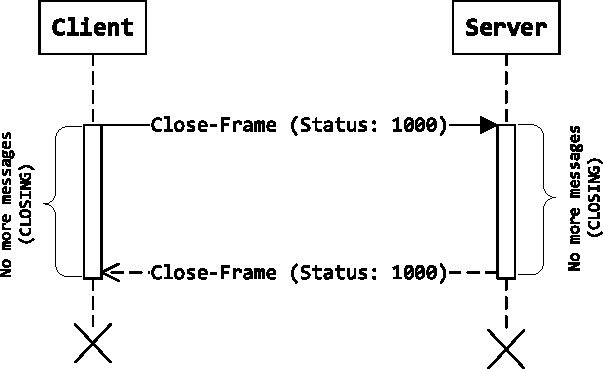
\includegraphics[scale=1]{img/closehandshake.pdf}
		\caption{Clientseitiger Closing-Handshake}
		\label{fig:wsClosingHandshake}
	\end{center}
\end{figure}

\noindent Abbildung \ref{fig:wsClosingHandshake} zeigt den schematischen Ablauf des Closing-Handshakes. Der Client initiiert diesen, indem er einen Closing-Frame mit dem Statuscode 1000 versendet. Der Server reagiert mit einer entsprechenden Antwort, wobei der Status aus dem ersten Frame übernommen wurde. Nachdem der Closing-Handshake abgeschlossen wurde befinden sich beide Endpunkte im Status \texttt{CLOSED} und die zugrundeliegende TCP-Verbindung kann beendet werden.

\subsection{Alternative Verfahren}\label{subsubsec:AlternativeVerfahren}
Die Kommunikation mittels HTTP basiert auf einem Request/Response Verfahren. Dabei sendet immer der Client eine Anfrage an einen Server. Dieser antwortet mit einer Statuszeile und entsprechendem Statuscode. Anschließend gilt die Übertragung als beendet und kann durch eine erneute Anfrage des Clients neu gestartet werden. Eine Möglichkeit Daten vom Server an den Client zu senden, ist in der Spezifikation von HTTP nicht vorgesehen. Verändert sich der Zustand einer serverseitigen Ressource, so kann der Client darüber bei einer reinen HTTP-Verbindung nur durch erneutes Anfragen informiert werden. Allerdings benötigen viele Anwendungsfälle diese Funktion. Aus diesem Grund wurde eine Vielzahl von Verfahren entwickelt, die diese Mechanismen abbilden sollen. Im Folgenden werden einige dieser Verfahren kurz vorgestellt und hinsichtlich ihrer Vor- und Nachteile gegenüber WebSocket analysiert.\\

\subsubsection{Polling}
Durch die vom W3C standardisierte API XMLHttpRequest (XHR) wurde im Jahr 2012 eine Möglichkeit geschaffen, mittels JavaScript HTTP-Requests zu konstruieren \autocite{whatwg_xmlhttprequest_2006}. Ein XHR-Objekt registriert verschiedene Methoden, welche bei einer Änderung des Objekts asynchron aufgerufen werden. Dadurch können Anfragen gesendet werden, ohne den weiteren Programmablauf zu blockieren. Dies bildet die technische Grundlage vieler moderner Web-Frontends, die unter dem Oberbegriff Ajax (\textit{Asynchronous JavaScript and XML}) zusammengefasst werden \autocite[26]{gorski_websockets_2015}. \\

\noindent Beim Polling-Verfahren wird eine Anfrage an den Server in festgelegten Zeitabständen wiederholt. Durch die Verwendung eines XHR-Objekts blockiert die Anwendung zwischen dem Absenden und Empfang der Serverantwort nicht. Liegt keine Änderung vor, so sendet der Server eine leere Antwort zurück. \\

\noindent Dieses Verfahren wird von allen Browsern unterstützt und bedarf keiner besonderen Kenntnisse. Allerdings ist der erzeugte Overhead je nach Einsatzszenario nicht zu unterschätzen. Auch die Belastung des Servers bei der Verarbeitung der eintreffenden Anfragen kann problematisch sein. Treten demnach viele Änderungen in kurzen Zeitabständen auf, so ist von der Verwendung eines einfachen Polling-Verfahrens abzuraten.

\subsubsection{Long-Polling}\label{subsubsec:Long-Polling}
Die regelmäßigen Abfragen des einfachen Pollings führen zu einem enormen Overhead. Um diesen zu reduzieren wird beim Long-Polling nur eine Antwort vom Server zurückgesendet, wenn eine Änderung vorliegt. Der Client reagiert umgehend mit einem neuen Request auf die Antwort des Servers. Die Verbindung bleibt dabei geöffnet, solange keine Änderung auftritt. Läuft die vordefinierte Wartezeit ab, so antwortet der Server auch hier mit einer leeren Nachricht \autocite[29]{gorski_websockets_2015}. \\

\noindent Das Long-Polling reduziert den Overhead gegenüber dem einfachen Polling-Mechanismus deutlich. Auf Grund des sofortigen Wiederaufbaus durch den Client wird eine nahezu andauernde Verbindung simuliert. Dennoch ist auch in diesem Fall der Overhead deutlich größer als bei der Verwendung einer WebSocket-Verbindung. Mit steigender Frequenz von Nachrichten nähert sich dieser an den Overhead des einfachen Pollings.

\subsubsection{Comet}\label{subsubsec:Comet}
Auf Grund diverser Limitierungen für Mehrbenutzeranwendungen, entwickelten sich Programmiermodelle, welche unter der Bezeichnung \textit{Comet} \autocite{russell_comet_2006} zusammengefasst wurden. Da es sich hierbei nicht um einen spezifizierten Standard handelt, wurde im Rahmen des CometD-Projekts der Dojo Foundation das Bayeux-Protokoll ins Leben gerufen. Ziel des Projekts ist die Reduzierung der Komplexität bei der Implementierung von Comet Anwendungen \autocite{russell_cometd_2007}. Um dies zu erreichen wurden Referenzimplementierungen des Bayeux-Protokolls in verschiedenen Programmiersprachen bereitgestellt. \\

\noindent Neben der Verwendung des Long-Polling Mechanismus zur ereignisgesteuerten Nachrichtenübertragung von Server zu Client, sieht das Bayeux-Protokoll auch Streaming-Techniken vor. Dabei wird die HTTP-Verbindung nach der Antwort des Servers auf den Request des Clients nicht geschlossen, sondern anhand des Connection-Headers \texttt{keep-alive} weiterhin offen gehalten. Somit können weitere Nachrichten vom Server an den Client gesendet werden, ohne dass eine erneute Anfrage durch den Client gestellt werden muss. Abbildung \ref{fig:wsBayeuxStream} illustriert die Übertragung einer Nachricht \texttt{M0} von einem Client, der in einem Webbrowser (\texttt{User Agent}) ausgeführt wird, zu einem Webserver \texttt{Origin Server}, auf welchem die serverseitige Implementierung des Bayeux-Protokolls ausgeführt wird. Die Übertragung erfolgt als HTTP Request und die korrespondierende Antwort des Servers als HTTP Response. Die Nachricht des Servers enthält dabei etwaige Bayeux-Events \texttt{E}. Nach der Übermittlung von \texttt{M1(E0)} wird die Verbindung nicht geschlossen, sodass der Server weiterhin Events an den Client übertragen kann. 

\begin{figure}[ht] 
	\begin{center}
		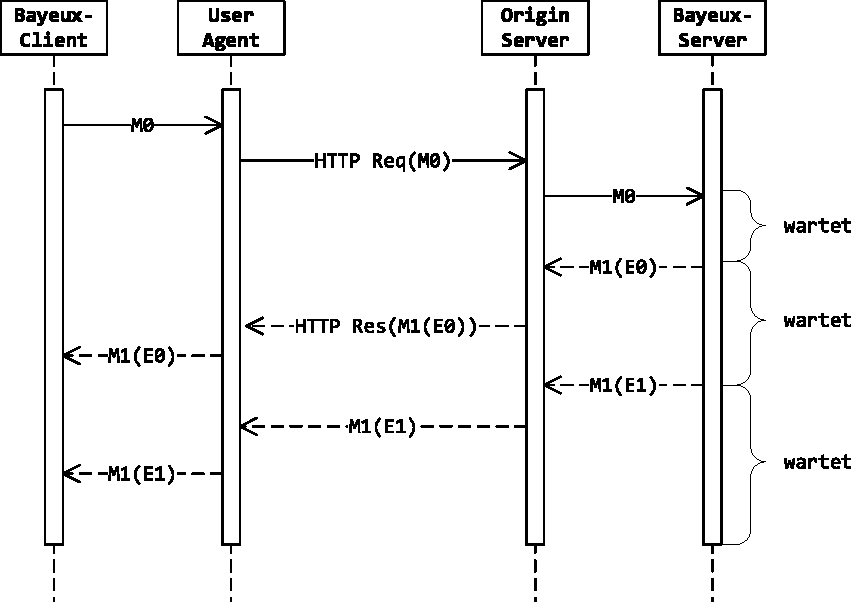
\includegraphics[scale=1]{img/bayeuxstream.pdf}
		\caption{HTTP-Streaming im Bayeux-Protokoll}
		\label{fig:wsBayeuxStream}
	\end{center}
\end{figure}


\noindent Allerdings muss die Verwendung von HTTP-Streaming von den User Agenten unterstützt werden, da unvollständige HTTP Responses für dieses Verfahren genutzt werden \autocite{russell_cometd_2007}. Um bidirektional kommunizieren zu können verwendet das Bayeux-Protokoll zwei HTTP-Verbindungen, wohingegen das WebSocket-Protokoll mit einer einzigen Verbindung arbeitet. Der größte Nachteil des Bayeux-Protokolls ist jedoch die fehlende Standardisierung durch eine etablierte Organisation. 

\subsubsection{Server-Sent Events}\label{subsubsec:Server-SentEvents}
Die bislang vorgestellten Verfahren bieten keine standardisierte API, die es Servern ermöglicht Daten über HTTP an eine Website zu senden. In HTML5 wurde dafür vom W3C die sogenannten \textit{Server-Sent Events (SSE)} eingeführt, welche ein \texttt{EventSource}-Objekt bereitstellen. Dieses sorgt auf der Clientseite dafür, dass Benachrichtigungen des Servers empfangen werden können. Dazu stellt der Browser drei Event-Handler bereit, die DOM-Events an die Anwendung weiterleiten \autocite[31]{gorski_websockets_2015}. Bei der Öffnung einer SSE-Verbindung wird der Event-Handler \texttt{onopen} aufgerufen, im Falle eines Fehlers der \texttt{onerror}-Handler. Kommen Nachrichten des Servers an, so wird der \texttt{onmessage}-Handler aktiviert \autocite{hickson_server-sent_2009}. Zu jedem Event-Handler werden entsprechende Methoden registriert, welche die Bearbeitung des jeweiligen Events übernehmen.\\

\noindent Server-Sent Events erzeugen keinen Overhead durch wiederholte Anfragen an den Server. Die Kommunikation von Server zu Client wird ermöglicht, ohne mehrere HTTP-Verbindungen zu öffnen. Allerdings handelt es sich hier um einen unidirektionalen Kanal von Server zu Client. Dies ist für Anwendungsfälle ausreichend, in denen lediglich der Server Informationen zu übermitteln hat. Beispiele hierfür wären u.a. das Hardware-Monitoring eines Server oder ein Newsticker. Sollen jedoch Daten in beide Richtungen übertragen werden, so ist die Verwendung von WebSockets die bessere Alternative. Insbesondere Mehrbenutzeranwendungen wie Spiele oder Chats, die auf kurze Latenzen angewiesen sind, profitieren von derem bidirektionalem Kommunikationskanal. \\

\noindent Die Vielfalt der Alternativen lässt darauf schließen, dass ein Bedarf für eine standardisierte Methode besteht, mit der Daten zwischen Client und Server bidirektional übertragen werden können. Dieser Bedarf führte zur Einführung der WebSockets, die als einzige auch für die Übertragung binärer Daten geeignet sind.
\newpage
\section{Die WebSocket-API}\label{sec:WebSocketAPI}
Neben der Protokollspezifikation durch das Standardisierungsgremium IETF, wurde auch eine passende API für die Verwendung von WebSockets definiert. Da es sich hierbei um eine Webtechnologie handelt die in Browsern Anwendung findet, obliegt deren Spezifierung dem W3C. Der erste Working Draft vom 23. April 2009 wurde von Ian Hickson eingereicht, einem der führenden Entwickler der Protokollspezifikation \autocite{hickson_web_2009}. Darin werden alle benötigten Eigenschaften und Funktionen der WebSocket-Schnittstelle definiert. Die Beschreibung erfolgt anhand der \textit{Web Interface Description Language} (\textit{Web IDL}), einer formalen Darstellung, die an die sprachlichen Konstrukte von ECMAScript bzw. JavaScript angelehnt ist. Dabei handelt es sich um eine Programmiersprache, die 1995 von Netscape Communications entwickelt und durch die European Computer Manufacturers Association (ECMA) unter der Bezeichnung ECMAScript standardisiert wurde \autocite{peyrott_brief_2017}. Alle Beispiele beziehen sich auf die aktuelle Version 8, die im Juni 2017 offiziell freigegeben wurde. Im Folgenden wird die geläufigere Bezeichnung JavaScript verwendet.

\subsection{Elemente der W3C WebSocket-API}
Das Erstellen eines WebSocket-Endpunkts erfolgt laut Spezifikation anhand des Konstruktors. Dieser empfängt die URL, zu welcher der Endpunkt sich verbinden soll und legt diese im read-only Attribut \texttt{url} ab. Optional empfängt der Konstruktor einen String oder ein String-Array, welches die unterstützten Sub-Protokolle enthält. \bigskip

\begin{lstlisting}[frame=single, language=JavaScript, caption=WebSocket anlegen und verbinden]
	var ws = new WebSocket(in DOMString url, in optional DOMString[] protocols);
\end{lstlisting}

\noindent Wird die URL nicht im korrekten Schema angegeben, so wird eine \texttt{DOMException} mit der Beschreibung \texttt{SyntaxError} ausgelöst. Falls Sub-Protokolle angegeben werden, so sendet der Client diese bei der Anfrage im HTTP-Headerfeld \texttt{Sec-WebSocket-Protocol}. Wenn Server und Client ein gemeinsames Protokoll vereinbaren konnten, wird es im schreibgeschützten Attribut \texttt{protocol} abgelegt. Etwaige Erweiterungen werden nach dem erfolgreichen Verbindungsaufbau im Attribut \texttt{extensions} abgelegt.
\subsubsection{WebSocket Lebenszyklus}
Jede WebSocket-Verbindung unterliegt einem Lebenszyklus. Die Spezifikation unterscheidet hier vier mögliche Zustände, die als konstante Zahlenwerte hinterlegt sind. Je nachdem in welchem Zustand sich der WebSocket gerade befindet, wird der Wert einer dieser Konstanten im Attribut \texttt{readyState} abgelegt \autocite{whatwg_html_2010}. \newpage
\begin{figure}[ht] \label{fig:wsLifeCycle}
	\begin{center}
		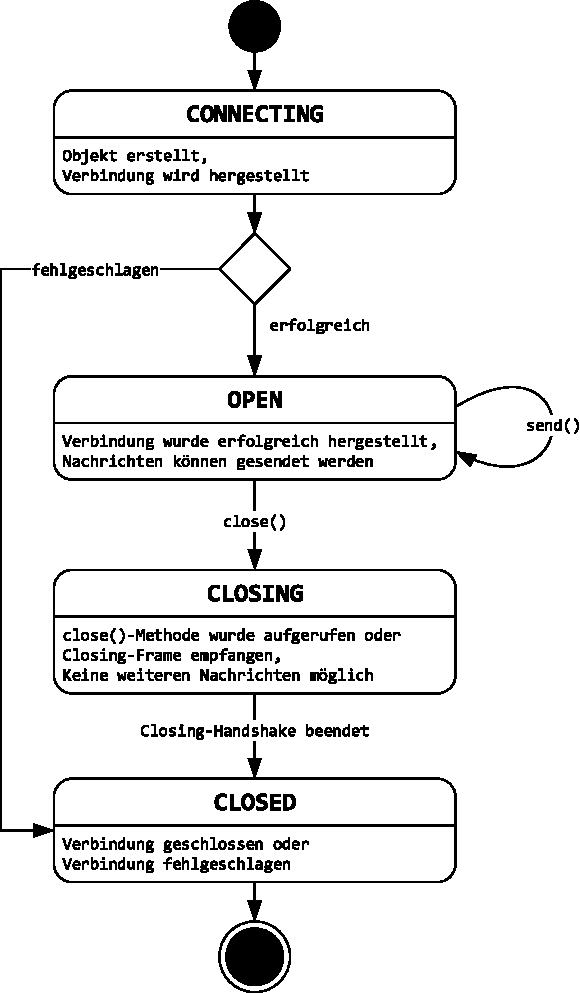
\includegraphics[scale=0.75]{img/wslifecycle.pdf}
		\caption{UML-Zustandsdiagramm des WebSocket Lifecycle}
		\label{fig:wsAPIZustand}
	\end{center}
\end{figure}

\noindent Die Implementierung in JavaScript spiegelt den Lebenszyklus eines WebSocket-Objekts gemäß der Beschreibung des W3C ab. So wird beim Anlegen des Objekts die Verbindung aufgebaut und lässt anschließend das Senden von Nachrichten zu. Durch den Aufruf der \texttt{close()}-Methode wird der Verbindungsaufbau eingeleitet. Das Schließen kann zudem optional mit Angabe eines Status-Codes (Tabelle \ref{tbl:wsCloseCodes}, S.\pageref{tbl:wsCloseCodes}) und einer textuellen Begründung erfolgen.\\

\begin{lstlisting}[frame=single, language=JavaScript, caption=WebSocket Lebenszyklus]
	var ws = new WebSocket("ws://echo.websocket.org"); // 0 = CONNECTING
	console.log(ws.readyState); // 1 = OPEN, wenn erfolgreich
	ws.send("Message"); // 1
	ws.close(1000, "Work done."); // 2 = CLOSING
	console.log(ws.readyState); // 3 = CLOSED
\end{lstlisting}

\subsubsection{Event-Handling}
Die Zustände eines WebSockets werden durch Events beeinflusst, die während der Kommunikation mit einem Endpunkt eintreffen. Diese werden von Event-Handlern empfangen und können anschließend verarbeitet werden. Die WebSocket API definiert die vier Event-Handler \texttt{onopen}, \texttt{onerror}, \texttt{onmessage} und \texttt{onclose}. Ein erfolgreicher Verbindungsaufbau löst das Event \texttt{open} aus, welches vom Event-Handler \texttt{onopen} verarbeitet wird. Fehler werden vom \texttt{onerror}-Event-Handler signalisiert. Wurde die Verbindung geschlossen oder konnte nicht geöffnet werden, so wird der \texttt{onclose}-Event-Handler ausgelöst. \\

\begin{lstlisting}[frame=single, language=JavaScript, caption=WebSocket Event-Handler]
	var ws = new WebSocket("ws://echo.websocket.org");
	// Registrieren des OnOpen-Handlers
	ws.onopen = function(){
		console.log("Verbindung hergestellt!");
	}
	// Registrieren des OnError-Handlers
	ws.onerror = function(e){
		console.log("Fehler aufgetreten: " + e.data);
	}	
	// Registrieren des OnMessage-Handlers
	ws.onmessage = function(e){
		showMessageInUI(e.data);
	}
	// Registrieren des OnClose-Handlers
	ws.onclose = function(e){
		console.log("CloseEvent erhalten - Verbindung wird abgebaut")
		console.log("Code: " + e.code);
		console.log("Grund: " + e.reason);
	}
\end{lstlisting} \vspace{-4mm}
\subsubsection{Kommunikation}
Empfangene Nachrichten können mittels des \texttt{onmessage}-Event-Handlers an die Anwendung weitergegeben werden. Entsprechend der Spezifikation des RFC6455 ermöglicht die WebSocket API das Senden von textuellen und binären Daten. Zur Unterscheidung verschiedener Arten binärer Daten stellt sie die Enumeration \texttt{BinaryType} bereit. Diese enthält die Werte \texttt{blob} und \texttt{ArrayBuffer}. Die Übermittlung der Daten erfolgt durch die Methode \texttt{send()}. Bei deren Aufruf wird das Attribut \texttt{bufferedAmount} um die Anzahl Bytes erhöht, die nicht in das Netzwerk übermittelt werden konnten \autocite{whatwg_html_2010}. \\

\begin{lstlisting}[frame=single, language=JavaScript, caption=WebSocket Nachrichten senden]
	var ws = new WebSocket("ws://echo.websocket.org");
	ws.send("Nachricht"); // als DOMString versenden
	ws.send(BlobUtils.fromString("Nachricht")) // als binary blob versenden
\end{lstlisting}

\subsection{Die Java\texttrademark{} API for WebSocket (JSR-356)}
\noindent Die WebSocket-APIs beschränken sich nicht nur auf JavaScript. Verschiedene Implementierungen des Standards ermöglichen dem Entwickler, WebSockets in seiner bevorzugten Programmiersprache zu nutzen. Laut des PopularitY of Programming Language (PYPL) Index ist Java der Oracle Corporation die weltweit beliebteste Programmiersprache \autocite{cabonnelle_pypl_2017}. Sie wurde 1990 von James Gosling mit seinem Team bei dem Unternehmen Sun Computers entwickelt. Die erste öffentlich zugängliche Version wurde 1995 veröffentlicht \autocite{smyth_brief_2009}. Aktuell ist Java 9 verfügbar. 

\subsubsection*{Java Community Process}
Soll eine neue Technologie in den Standardumfang von Java aufgenommen werden, so muss diese den Community Prozess (JCP) durchlaufen \autocite{oracle_corporation_java_2017}: \\

\begin{figure}[ht] 
	\begin{center}
		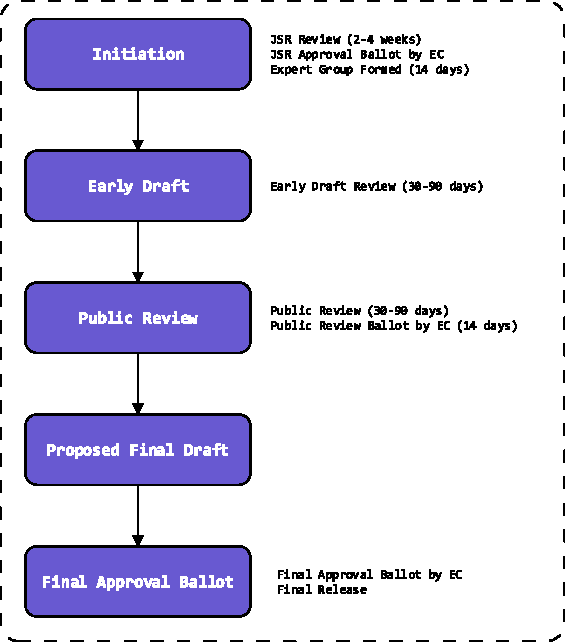
\includegraphics[scale=1]{img/jsr.pdf}
		\caption{JSR Approval Timeline}
		\label{fig:wsAPIJSRApproval}
	\end{center}
\end{figure}

\noindent In Phase 1 können Mitglieder des JCP einen Vorschlag zur Aufnahme einer Erweiterung machen. Diese werden als \textit{Java Specification Request} (JSR) bezeichnet. Wird der JSR vom \textit{Executive Committee} (EC) angenommen, so wird bis Phase 2 eine Expertengruppe gebildet, die einen Early Draft erstellt. Darauf aufbauend entwickelt diese Gruppe einen Public Draft, der in Phase 3 öffentlich eingesehen und kommentiert werden kann. Der Entwurf wird dann entsprechend überarbeitet und eine finale Version eingereicht. Zudem wird eine Referenzimplementierung (RI)  und das Technology Compatibility Kit (TCK) erstellt, welches Tests und Tools bereitstellt um Implementierungen auf Konformität mit dem JSR zu prüfen. Abschließend stimmt das EC noch über die Aufnahme in die Standardbibliothek ab. Befindet sich der JSR dann im produktiven Betrieb, können in der Maintenance Phase Updates und Änderungen des JSR beantragt und eingepflegt werden \autocite{oracle_corporation_java_2017}.\\

\noindent Der JSR 356 trägt die Bezeichnung Java\texttrademark API for WebSocket und regelt die Aufnahme der WebSocket-Technologie in die Standardbibliothek der Java Enterprise Edition (JEE). Er befindet sich aktuell in der 4. Phase und ist seit dem 22. Mai 2013 offizieller Bestandteil seit JEE 7. Die folgenden Beispiele verwenden die achte Version von Java.

\subsubsection{Grundlagen}
Alle Klassen und Interfaces zur Impementierung von WebSocket-Clients und Servern wurden für Java in dem Paket \texttt{javax.websocket} zusammengefasst. Für einen WebSocket-Client, der weder im Browser noch in einem anderen Framework zum Einsatz kommt, kann in Java die Open-Source Referenzimplementierung \textit{Tyrus} von Oracle verwendet werden. Nachfolgende Beispiele verwenden das aktuellste Release 1.12. Die Bereitstellungen erfolgen über Maven: 
\vspace{-5mm}
\begin{center}\parbox{0pt}{
	\begin{tabbing}
		\texttt{<depen}\=\texttt{dency>}\\
		\>\texttt{<groupId>javax.websocket</groupId>}\\
		\>\texttt{<artifactId>javax.websocket-api</artifactId>}\\
		\>\texttt{<version>1.1</version>}\\
		\>\texttt{<scope>provided</scope>}\\
		\texttt{</dependency>}\\
		\texttt{<dependency>}\\
		\>\texttt{<groupId>org.glassfish.tyrus.bundles</groupId>}\\
		\>\texttt{<artifactId>tyrus-standalone-client</artifactId>}\\
		\>\texttt{<version>1.12</version>}\\
		\texttt{</dependency>}
	\end{tabbing}}
\end{center}
\noindent Für die Implementierung eines WebSocket-Serverendpunkts wird zudem ein Webserver benötigt, der die WebSocket-API implementiert. Für Java gibt es hier eine Vielzahl von Alternativen zur Auswahl:

\begin{itemize}
\singlespacing{
	\item Apache Tomcat ab Version 7.0.56 \autocite{the_apache_foundation_apache_2014}
	\item GlassFish Server ab Version 4.1 \autocite{oracle_corporation_glassfish_2014}
	\item Grizzly ab Version 2 \autocite{oracle_corporation_project_2017}
	\item Eclipse Jetty ab Version 7 \autocite{the_eclipse_foundation_jetty_2016}
	\item Netty ab Version 4.0 \autocite{lee_netty.news_2011}
}
\end{itemize}

\subsubsection*{Ansätze der Programmierung}
Die Java\texttrademark API for WebSocket kann auf zwei unterschiedliche Weisen verwendet werden. Der programmatische Ansatz sieht die Vererbung der \texttt{Endpoint} Klasse der API vor. Dabei müssen u.a. die Methoden der Oberklasse überschrieben und Funktionen auf Events registriert werden. \autocite[9]{coward_java_2014}:\smallskip

\begin{lstlisting}[frame=single, language=Java, caption=Java: Programmatischer Ansatz]
	public class MyWebSocketClient extends Endpoint {
		@Override
		public void onOpen(Session session) {
			session.addMessageHandler(new MessageHandler.Whole<String>() {
				@Override
				public void onMessage(String message) {
					// Verarbeitung der Nachricht
				}
			});
		}
	}
\end{lstlisting}

\noindent Der Einsatz von Annotationen transformiert einfache Java-Objekte zu WebSocket Endpunkten. Handelt es sich um eine Annotation auf Klassenebene, so können diverse Konfigurationsparameter angegeben werden. Alle Informationen sind somit an einer Stelle gesammelt und auf eine Konfigurationsklasse kann in vielen Fällen verzichtet werden.\smallskip

\begin{lstlisting}[frame=single, language=Java, caption=Java: Annotationen,label=lst:ServerAnnotation]
	@ServerEndpoint( value = "/endpoint", subprotocols = {"chat"})
	public class MyWebSocketServer { ... }
\end{lstlisting}

\noindent Die nachfolgenden Code-Beispiele sind immer annotations-basiert, aufgrund besserer Lesbarkeit, verkürzter Schreibweise und der einfachen Verständlichkeit. \vspace{-3mm}

\subsubsection*{Erzeugung eines WebSockets}
\noindent Clientseitige Endpunkte werden mit der Annotation \texttt{@ClientEndpoint} versehen. Die Konstruktion eines WebSockets erfolgt hier durch die Erzeugung eines Container-Objekts, welches anschließend zum Verbindungsaufbau verwendet wird.\smallskip

\begin{lstlisting}[frame=single, language=Java, caption=Java Client: Verbindungsaufbau]
	@ClientEndpoint
	public class MyClient {
		public MyClient(URI hostPath){
			// Container-Objekt erstellen
			WebSocketContainer wsc = ContainerProvider.getWebSocketContainer();
			// Verbindung fuer Endpunkt MyClient herstellen
			wsc.connectToServer(this, hostPath);
		} }
\end{lstlisting}

\noindent Die Erstellung des Objekts ist nur dann erfolgreich, wenn die WebSocket-Verbindung aufgebaut werden konnte. Ein WebSocket-Server wird mit der Annotation \texttt{@ServerEndpoint} gekennzeichnet. Sowohl bei Server- als auch bei Clientendpunkten können verschiedene Konfigurationsparameter verwendet werden (siehe Listing \ref{lst:ServerAnnotation}). Der Parameter \texttt{value} gibt dabei den relativen Pfad an, unter dem der WebSocket-Endpunkt erreichbar ist. Wird die Anwendung auf einem lokalen WebServer ausgeführt und ihre Bezeichnung lautet \texttt{example}, so ist die Anwendung erreichbar unter \url{ws://localhost[:port]/example/endpoint}. Unterstützte Subprotokolle können optional mittels des Parameters \texttt{subprotocols} angegeben werden. Falls die Anwendung eigene Java-Objekte oder komplexere Datentypen übertragen soll, so müssen Encoder- bzw. Decoder-Klassen angegeben werden. Diese werden im Abschnitt \ref{subsubsec:DeEnCoding} näher erläutert.
%\noindent Der Zugriff auf etwaige Erweiterungen oder Subprotokolle erfolgt in Java durch das \texttt{Session} Objekt. \\
%
%\begin{lstlisting}[frame=single, language=Java, caption=Java Client: Erweiterungen und Subprotokolle]
%	@OnOpen
%	public void onOpen(Session session){
%		// Erweiterungen
%		List<Extension> ext = session.getNegotiatedExtensions();
%		// Subprotokoll
%		String subp = session.getNegotiatedSubprotocol();
%	}
%\end{lstlisting}
\subsubsection*{Event-Handling}
\noindent Durch die Verwendung der Annotationen erfolgt in Java keine manuelle Deklaration der Handler. Eine Methode, die ein bestimmtes Event bearbeitet, wird durch Angabe der jeweiligen Annotation zu einem EventHandler transformiert.\\
\begin{lstlisting}[frame=single, language=Java, caption=Java: EventHandler]
	@OnOpen
	public void init(Session session, EndpointConfig config){
		// Session und Konfiguration in Variable speichern
	}
	
	@OnError
	public void error(Throwable t) {
		System.out.println("Fehler aufgetreten: " + t.getMessage());
	}
	
	@OnClose
	public void close(CloseReason c) {
		System.out.println("Die Verbindung wurde geschlossen.");
		System.out.println("Code: " + c.getCloseCode());
		System.out.println("Grund: " + c.getReasonPhrase()); 
	}
	
	@OnMessage
	public void incoming(String msg){
		System.out.println("Neue Nachricht empfangen: " + msg);
	}
	
\end{lstlisting}

\noindent Die Java\texttrademark{} API for WebSocket sieht dafür die Annotationen \texttt{@OnOpen}, \texttt{@OnError}, \texttt{@OnMessage} und \texttt{@OnClose} vor. Jede auf diese Weise deklarierte Methode ermöglicht die Angabe einiger Parameter. Die aktuell verwendete \texttt{Session} kann dabei immer empfangen werden. \\

\subsubsection{Kommunikation}\label{subsubsec:javaKommunikation}
Der RFC6455 definiert Ping- und Pong-Frames, durch die beispielsweise geprüft werden kann, ob ein Endpunkt noch erreichbar ist oder um eine inaktive Verbindung aufrechtzuerhalten. Allerdings spezifiert die W3C WebSocket API keine Möglichkeit, diese Art von Control-Frames zu versenden. Die Java API hingegen stellt dafür die Methoden \texttt{sendPing()} und \texttt{sendPong()} zur Verfügung, die ein \texttt{ByteBuffer}-Objekt als Parameter empfangen, über welches Nutzdaten mit bis zu 125 Byte angehängt werden können. Diese Limitierung wird aufgrund der im RFC6455 definierten Größe von Control-Frames durch eine \texttt{IllegalArgumentException} sichergestellt.\\

\begin{lstlisting}[frame=single, language=Java, caption=Java: Ping/Pong Nachrichten, label=lst:PingPong]
	public void sendPing(ByteBuffer applicationData) throws IOException, IllegalArgumentException

	public void sendPong(ByteBuffer applicationData) throws IOException, IllegalArgumentException

	@OnMessage
	public void catchPong(PongMessage pong, Session session){ ... }
\end{lstlisting}

\noindent Die Antwort auf eine eingehende Ping-Nachricht muss nicht durch den Entwickler erfolgen. Die Implementierungen der Java WebSocket-API stellen sicher, dass eine korrespondierende Pong-Nachricht so bald wie möglich zurückgesendet wird. In Listing \ref{lst:PingPong} ist die Methode \texttt{catchPong} definiert, die als Parameter ein \texttt{PongMessage}-Objekt empfängt. Durch sie ist es möglich, die Antwort einer zuvor gesendeten Ping-Nachricht weiter zu verarbeiten. Beispielsweise können so Messungen der \textit{Round Trip Time} (RTT) durchgeführt werden. Allerdings ist deren Aussagekraft nur bedingt gegeben, da diese bei größeren Nachrichten stark abweichen können \autocite[116]{coward_java_2014}. Das Senden einer Pong-Nachricht ohne vorangegangenen Ping kann genutzt werden, um einen unidirektionalen \textit{Heartbeat} abzubilden. Ein Endpunkt antwortet spezifikationsgemäß nicht auf eine eintreffende Pong-Nachricht, es sei denn, eine entsprechende Methode wurde dafür bereitgestellt. \\

\noindent Das Senden und Empfangen sowohl textueller als auch binärer Daten ist ebenfalls in der Java WebSocket API definiert. Die grundlegendsten Datentypen, die dabei eingesetzt werden können sind \texttt{String}, \texttt{ByteBuffer} und \texttt{byte[]} \autocite[30]{coward_java_2014}. Darüber hinaus ist es möglich, komplexere Datenstrukturen oder eigene Objekte zu versenden. Dies setzt jedoch entsprechende Decoder- und Encoder-Klassen voraus. Liegen Daten zum Zeitpunkt des Versendens noch nicht vollständig vor oder können aufgrund ihrer Größe nicht in einem einzigen Frame übertragen werden, so kann auf Methoden zurückgegriffen werden, die das partielle Übertragen von Nachrichten ermöglichen. Aufgrund der protokolleigenen Fragmentierung können diese Teilnachrichten von den tatsächlich übertragenen Fragmenten abweichen. Wird der letzte Teil einer Nachricht übertragen, so muss das \texttt{isLast} Flag der jeweiligen \texttt{send}-Methode gesetzt werden. Das Versenden erfolgt immer über die \texttt{RemoteEndpoint} Schnittstelle, die man durch ein \texttt{Session} Objekt erhält. \\

\begin{lstlisting}[frame=single, language=Java, caption=Java: Synchrone Nachrichtenübertragung]
	public void sendMessages(Session session){
	
		RemoteEndpoint.Basic rEndpoint = session.getBasicRemote();
		
		// Textnachricht als String
		rEndpoint.sendText("Message");
		
		// Binaere Daten senden
		rEndpoint.sendBinary(ByteBuffer.wrap("Message".getBytes()));
		
		// Partielles Senden einer Textnachricht
		String part1 = "Mess";
		String part2 = "age";
		boolean isDone = false;
		rEndpoint.sendText(part1, isDone);
		rEndpoint.sendText(part2, !isDone);
	}
\end{lstlisting}

\noindent Die bisher vorgestellten Methoden zum Nachrichtenversand blockieren solange, bis der gesamte Payload übertragen wurde. Soll die Applikation hingegen weitere Aufgaben während des Sendens erledigen können, so muss auf die Funktionen der Schnittstelle \texttt{RemoteEndpoint.Async} zurückgegriffen werden. Beispiele für den Einsatz asynchroner Verarbeitung finden sich häufig. So soll eine grafische Oberfläche beim Versand einer sehr großen Nachricht weiterhin reagieren können. Um Nachrichten asynchron zu übertragen, stellt die API zwei Varianten zur Verfügung. \\

\begin{lstlisting}[frame=single, language=Java, caption=Java: Future und Handler]
	// Liefert Future-Objekt zurueck
	public Future<Void> sendText(String text);
	
	// Benoetigt SendHandler
	public void sendText(String text, SendHandler handler);

\end{lstlisting}

\noindent Der erste Weg besteht aus dem Senden einer WebSocket-Nachricht \textit{by future} \autocite[119]{coward_java_2014}. Der Sinn und Zweck eines \texttt{Future}-Objekts ist die Nachverfolgung des Versendungsstatus durch den Aufruf der zugehörigen Methoden. So kann mittels \texttt{isDone()} geprüft werden, ob die Nachricht versand wurde. Die Methode \texttt{cancel()} bricht eine ausstehende Übertragung ab. Im Unterschied zur synchronen Nachrichtenübertragung werden etwaige Ausnahmen oder Fehler nicht automatisch zurückgemeldet. Diese können nur durch 
\texttt{Future.get()} ermittelt werden. Diese Methode blockiert die weitere Ausführung, bis die Nachricht übermittelt wurde oder ein Fehler aufgetreten ist. \\

\noindent Die zweite Möglichkeit Nachrichten asnychron zu übermitteln erfordert die Bereitstellung eines \textit{callback} Objekts. Dabei handelt es sich um eine Implementierung der \texttt{SendHandler}-Schnittstelle, die beim Eintreffen eines Ereignisses ausgelöst wird. Man spricht vom Senden einer Nachricht \textit{with handler}.\smallskip

\begin{lstlisting}[frame=single, language=Java, caption=Java: Callback Interface SendHandler]
public class MyHandler implements SendHandler {
	@Override
	public void onResult(SendResult arg0) {
		// Verarbeiten des Ergebnisses
	}
}
\end{lstlisting}

\noindent Beide Varianten der asynchronen Nachrichtenübermittlung können sowohl textuelle, als auch binäre Daten übertragen. Für das Senden komplexer Strukturen oder eigener Objekte wird auch hier ein Encoder benötigt. Ping- bzw. Pong-Nachrichten können nicht asynchron übertragen werden. Die Notwendigkeit asynchroner Übertragung ist in diesem Fall auch nicht gegeben, da diese Control-Frames maximal 125 Byte Nutzdaten enthalten können und dementsprechend selbst bei geringen Bandbreiten unverzüglich übermittelt werden \autocite[120]{coward_java_2014}. Die Entscheidung für eine der beiden Varianten der asynchronen Nachrichtenübertragung hängt von verschiedenen Faktoren ab. Soll nur eine kleine Anzahl anderer Aufgaben während des Sendevorgangs erledigt werden, so kann die Nachricht \textit{by future} versendet, anschließend andere Aufgaben gestartet und nach deren Beendigung durch den Aufruf der \texttt{get()}-Methode auf die Sendebestätigung gewartet werden. Dieser Ansatz blockiert dadurch einen laufenden Thread. Folgen jedoch weitere Aufgaben nach dem Versand der Nachricht, deren Bearbeitung Vorrang hat, so sollten \texttt{Handler} eingesetzt werden. Die Benachrichtigung einer eintreffenden Sendungsbestätigung muss hierbei durch einen eigenen Thread der zugrundeliegenden WebSocket-Implementierung erfolgen \autocite[123]{coward_java_2014}. Dieser Ansatz blockiert dadurch nicht den laufenden Thread des eigenen Programms. Zu beachten ist weiterhin, dass lediglich durch die Verwendung des \texttt{Future}-Ansatzes das Senden einer Nachricht abgebrochen werden kann.

\subsubsection{En- und Decoding}\label{subsubsec:DeEnCoding}
Die W3C WebSocket-API definiert lediglich textuelle und binäre Datentypen zur Übermittlung von Nutzdaten und entspricht damit den Anforderungen, die im RFC6455 für das WebSocket-Protokoll festgelegt wurden. Die Java WebSocket-API stellt hierfür standardisierte Methoden bereit, die das Senden eines \texttt{String}-Objekts oder binärer Datentypen wie \texttt{ByteBuffer} bzw. \texttt{byte[]} ermöglichen. In vielen Fällen ist es jedoch von Vorteil, komplexere Datentypen oder eigene Objekte übertragen zu können. Dafür wurde die \texttt{send}-Methode der \texttt{RemoteEndpoint}-Schnittstelle überladen, sodass sie einen Parameter vom Typ \texttt{Object} empfängt. Mit Hilfe dieser Methode lassen sich demnach Objekte eines beliebigen Datentyps versenden. Da das WebSocket-Protokoll aber lediglich textuelle oder binäre Daten kennt, müssen alle komplexeren Objekte in eine dieser beiden Formen gebracht werden. Zu diesem Zweck wurden die Schnittstellen \texttt{Encoder} und \texttt{Decoder} im Paket \texttt{javax.websocket} bereitgestellt. Über untergeordnete Schnittstellen kann zwischen der Umwandlung in textuelle oder binäre Daten gewählt werden. \medskip

\begin{lstlisting}[frame=single, language=Java, caption=Java: Encoder Interface]
	public interface Encoder {
		// Aufruf bei Verbindungsaufbau
		void init(EndpointConfig config);
		// Aufruf bei Verbindungsabbau
		void destroy();
		// Sub-Interfaces mit jeweiliger encode-Methode
		interface Text<T> extends Encoder { String encode(T object) throws EncodeException; }
		interface Binary<T> extends Encoder { ByteBuffer encode(T object) throws EncodeException; }
	}
\end{lstlisting}

\noindent Die textuelle Enkodierung eines Objekts mit der Klassenbezeichnung \texttt{MyObject} erfolgt demnach über eine Klasse, die das \texttt{Encoder.Text<MyObject>} Interface implementiert. Sowohl die Enkodierung, als auch die Dekodierung erfolgen automatisch und müssen nicht vom Entwickler ausgelöst werden. Die Enkodierung von \texttt{MyObject} erfolgt beim Aufruf der \texttt{send}-Methode. \medskip

\begin{lstlisting}[frame=single, language=Java, caption=Java: Decoder Interface]
	public interface Decoder {
	
		// Aufruf bei Verbindungsaufbau
		void init(EndpointConfig config);
		
		// Aufruf bei Verbindungsabbau
		void destroy();
		
		// Sub-Interfaces mit jeweiliger decode- und willDecode-Methode
		interface Binary<T> extends Decoder {
			T decode(ByteBuffer bytes) throws DecodeException;
			boolean willDecode(ByteBuffer bytes);
		}
		
		interface Text<T> extends Decoder {
			T decode(String s) throws DecodeException;
			boolean willDecode(String s);
		}
	}
\end{lstlisting}

\noindent Ein Endpunkt, der nur über eine \texttt{@OnMessage}-Methode verfügt, die als Parameter ein Objekt vom Typ \texttt{MyObject} empfängt, muss beim Erhalt einer textuellen Nachricht diese dekodieren. Dies erfolgt über eine Klasse, die das \texttt{Decoder.Text<MyObject>}-Interface implementiert hat. Dazu ist es zunächst notwendig, zu überprüfen ob die Dekodierung möglich ist. Dies wird über die Methode \texttt{willDecode} sichergestellt. Anschließend wird das erwartete Objekt aus dem empfangenen Text dekodiert.\medskip

\noindent Damit ein WebSocket-Endpunkt Nachrichten enkodieren oder dekodieren kann, müssen diese Klassen bekannt gemacht werden. Dies erfolgt durch deren Angabe als Parameter in der jeweiligen Klassenannotation. Sollen verschiedene Objekte versendet oder empfangen werden, so müssen entsprechende Encoder- und Decoderklassen bereitgestellt werden. Die Auswahl der passenden Klasse erfolgt anhand ihrer Reihenfolge in der Klassenannotation.\medskip

\begin{lstlisting}[frame=single, language=Java, caption=Java: Angabe der Encoder- und Decoder-Klassen]
	@ClientEndpoint(encoders = { MyObjectEncoder.class }, 
								decoders = { MyObjectDecoder.class })
	public class MyWebSocketClient { ... }
\end{lstlisting}

\noindent Jede WebSocket-Verbindung erhält eine eigene Instanz der Encoder- und Decoder-Klassen. Dadurch wird sichergestellt, dass niemals mehr als ein Thread in der \texttt{decode()} oder \texttt{encode()} Methode aktiv ist \autocite[82]{coward_java_2014}. 

\subsubsection{Konfiguration und \texttt{Session}}
Eine der zentralen Komponenten der Java WebSocket-API ist die \texttt{EndpointConfig} Schnittstelle. Durch sie können einem Endpunkt diverse Meta-Daten übermittelt werden, die den gemeinsamen Zustand aller verbundenen Endpunkte repräsentieren. Je nach Art des Endpunktes wird weiterhin zwischen \texttt{ClientEndpointConfig} und \texttt{ServerEndpointConfig} unterschieden. Die Parameter sind bei der Verwendung von Annotationen in der jeweiligen Klassenannotation anzugeben. Sie werden zum Zeitpunkt der Bereitstellung dazu verwendet, um eine entsprechende Instanz der zugehörigen Endpunktkonfiguration zu erstellen. Diese Konfiguration kann als optionaler Parameter von den Event-Handlern empfangen werden.\\

\noindent Die Methoden der übergeordneten \texttt{EndpointConfig} Schnittstelle sind sowohl für Server-, als auch für Clientendpunkte verfügbar. Durch sie können die konfigurierten Encoder- und Decoder-Klassen sowie ein \texttt{Map} Objekt abgerufen werden. Die \texttt{Map} kann vom Entwickler genutzt werden, um applikationsspezifische Objekte und Informationen abzulegen. \medskip

\begin{lstlisting}[frame=single, language=Java, caption=Java: EndpointConfig]
	public interface EndpointConfig{
		// Liste aller Encoder-Klassen
		List<Class<? extends Encoder>> getEncoders()
		// Liste aller Decoder-Klassen
		List<Class<? extends Decoder>> getDecoders()
		// Editierbare Map
		Map<String,Object> getUserProperties()
	}
\end{lstlisting}
\noindent Die Konfigurationsschnittstelle des Clients ermöglicht den Zugriff auf clientspezifische Eigenschaften wie die bevorzugten Subprotokolle, Erweiterungen und den Konfigurator. Der Konfigurator ist eine Klasse, die Modifikationen an der HTTP-Anfrage sowie eine manuelle Auswertung der zugehörigen Antwort des Servers ermöglicht.

\begin{mdframed}[hidealllines=true,backgroundcolor=lightgray!20]
\paragraph{Subprotokolle und Erweiterungen}
Die Spezifikation des WebSocket-Protokolls ermöglicht die Bereitstellung von Subprotokollen und Erweiterungen. Die verwendeten HTTP-Felder im Opening-Handshake lauten \texttt{Sec-WebSocket-Protocol} und \texttt{Sec-WebSocket-Extensions}. Subprotokolle werden dabei als einfache \texttt{Strings} angegeben und durch Kommata getrennt. Bei der Vergabe eines eigenen Namens für ein Subprotokoll sollte beachtet werden, dass es nicht zu einer Überschneidung mit den bei der IANA registrierten Bezeichnungen kommt. Werden WebSocket-Frames um zusätzliche Informationen erweitert, um beispielsweise den Inhalt der Nutzdaten näher zu beschreiben, so spricht man von \texttt{Extensions} \autocite[102]{coward_java_2014}. Verwendet eine Applikation Subprotokolle oder Erweiterungen, so werden diese ebenfalls in der Klassenannotation hinterlegt.\\
\end{mdframed}
\noindent Für das Hinzufügen oder Ändern der HTTP-Header muss die verwendete Konfiguratorklasse von der Klasse \texttt{ClientEndpointConfig.Configurator} abgeleitet werden. Ein häufiger Anwendungsfall ist die Erweiterung der HTTP-Anfrage um applikations- oder frameworkspezifische Informationen für zusätzliche Funktionen \autocite[104]{coward_java_2014}. In Listing \ref{lst:cConf} ist ein solcher Fall beispielhaft dargestellt.\medskip

\begin{lstlisting}[frame=single, language=Java, caption=Java: ClientEndpointConfig Konfigurationsklasse, label=lst:cConf]
	public class MyClientConfig extends ClientEndpointConfig.Configurator {

		@Override
		public void afterResponse(HandshakeResponse hr) {
			// Pruefen, ob Feature aktiviert werden konnte
			boolean activated = hr.getHeaders().get("My-Feature-Field").get(0)
												.equals("activated"); 	
			// Aktivieren des Features oder Fallback
			super.afterResponse(hr);
		}

		@Override
		public void beforeRequest(Map<String, List<String>> headers) {
			// HTTP-Headerfeld fuer "MyFeature" erzeugen
			List<String> featureParam = new ArrayList<String>();
			featureParam.add("enable");
			// HTTP-Header erweitern
			headers.put("My-Feature-Field", featureParam);
			super.beforeRequest(headers);
	}	}
\end{lstlisting}

\noindent Die Konfiguration des Server durch die \texttt{ServerEndpointConfig} Schnittstelle bietet ebenfalls den Zugriff auf einen Konfigurator. Zudem ist es möglich die unterstützten Subprotokolle und Erweiterungen des Servers sowie die Klasse des Endpunkts abzurufen. Die Ermittlung des relativen Pfads des Serverendpunkts wird in Abschnitt \ref{subsubsec:apiPathMapping} detailliert behandelt. \\

\noindent Der Konfigurator der \texttt{ServerEndpointConfig} stellt zusätzlich diverse Methoden bereit, über die der Verbindungsaufbau gezielt gesteuert werden kann. So kann ein passendes Subprotokoll oder eine Erweiterung gewählt, die Erzeugung einer neuen Instanz manuell durchgeführt und in den Handshake selbst eingegriffen werden. Die Methode \texttt{checkOrigin()} prüft, ob der für Browserclients verbindliche HTTP-Origin-Header auf den selben Webserver verweist, auf dem der Serverendpunkt ausgeführt wird \autocite[107]{coward_java_2014}. Eine Anpassung ist meist nicht notwendig. Listing \ref{lst:sConf} zeigt den Konfigurator des Serverendpunkts, welcher den modifizierten Opening-Handshake des Clients aus Listing \ref{lst:cConf} bearbeitet. Dazu wird in der Methode \texttt{modifyHandshake()} die Anfrage des Clients auf das entsprechende Feld geprüft und die Antwort des Servers vor dem Versenden angepasst. \medskip

\begin{lstlisting}[frame=single, language=Java, caption=Java: ServerEndpointConfig Konfigurationsklasse, label=lst:sConf]
	public class MyServerConfig extends ServerEndpointConfig.Configurator {
	
		@Override // Hier kann die Pruefung des Origin-Headers durchgefuehrt werden
		public boolean checkOrigin(String originHeaderValue) { ... }
		
		@Override // Hier kann die Erzeugung einer neuen Instanz angepasst werden
		public <T> T getEndpointInstance(Class<T> endpointClass) throws InstantiationException { ... }
		
		@Override // Hier kann der Standardablauf der Wahl der Erweiterung veraendert werden
		public List<Extension> getNegotiatedExtensions(List<Extension> installed, List<Extension> requested) { ... }
		
		@Override // Hier kann der Standardablauf der Protokollwahl veraendert werden
		public String getNegotiatedSubprotocol(List<String> supported, List<String> requested) { ... }
		
		@Override
		public void modifyHandshake(ServerEndpointConfig sec, HandshakeRequest request, HandshakeResponse response) {
			// Anfrage auf zusaetzliches Header-Feld pruefen
			boolean activateMyFeature = request.getHeaders().get("My-Feature-Field").get(0).equals("enable");
		
			if(activateMyFeature) {
				// HTTP-Headerfeld fuer "MyFeature" erzeugen
				List<String> featureParam = new ArrayList<String>();
				featureParam.add("activated");
				
				// HTTP-Antwort-Header erweitern
				response.getHeaders().put("My-Feature-Field", featureParam);
		}	}	
	}
\end{lstlisting}

\noindent Durch den Einsatz der \texttt{EndpointConfig}-Klassen werden Einstellungen getroffen, die übergreifend für alle verbundenen Endpunkte gelten. Das \texttt{Session}-Objekt hingegen repräsentiert alle Einstellungen und Zustände, bezüglich einer einzelnen WebSocket-Verbindung. Für einen WebSocket-Client exisitiert nur eine \texttt{Session}, wohingegen ein WebSocket-Server Zugriff zu allen verbundenen Clients hat. Ein \texttt{Session}-Objekt wird bei einer erfolgreich aufgebauten Verbindung erstellt und kann über die mit \texttt{@OnOpen} gekennzeichnete Methode empfangen werden. Durch den Aufruf der Methode \texttt{getId()} lässt sich ein eindeutiger Bezeichner zur Identifizierung einer \texttt{Session} ermitteln. Weiterhin können zur Laufzeit die Methoden zur Bearbeitung von Events ermittelt, hinzugefügt oder entfernt werden. Ändert sich im Laufe einer Verbindung beispielsweise die Art, wie ein Client Nachrichten bearbeiten soll, so kann durch den Aufruf der \texttt{removeMessageHandler}- sowie \texttt{addMessageHandler}-Methode des zugehörigen \texttt{Session}-Objekts der \texttt{@OnMessage}-Handler ausgetauscht werden. Wie bereits in Abschnitt \ref{subsubsec:javaKommunikation} dargestellt, erfolgt das Senden von Nachrichten über \texttt{Basic}- oder \texttt{Async}-Objekte des \texttt{RemoteEndpoint}-Interfaces. Diese werden durch die Methoden \texttt{getBasicRemote()} respektive \texttt{getAsyncRemote()} der zugehörigen \texttt{Session} bereitgestellt. \\

\noindent Die Konfiguration verschiedener verbindungsspezifischer Eigenschaften kann ebenfalls über das \texttt{Session}-Objekt verändert werden. Auf einige dieser Merkmale ist der Zugriff lediglich lesend möglich, da deren Werte während des Verbindungsaufbaus zwischen Server und Client ausgehandelt werden. Hierbei handelt es sich um die Liste der verfügbaren Subprotokolle und Erweiterungen, die verwendete Protokollversion und den authentifizierten Benutzer, repräsentiert durch ein Java \texttt{UserPrincipal}-Objekt. Des weiteren kann geprüft werden, ob die Verbindung verschlüsselt erfolgt. Schreibender Zugriff ist auf folgende Eigenschaften möglich: 

\begin{description}
	\item[\texttt{userProperties}] Ein \texttt{map}-Objekt, in dem benutzerspezifische Schlüssel-Werte-Paare gespeichert werden können.
	\item[\texttt{maxBinaryMessageSize}] Beschränkt die Größe einer ankommenden binären Nachricht. 
	\item[\texttt{maxTextMessageSize}] Beschränkt die Größe einer ankommenden textuellen Nachricht. 
	\item[\texttt{maxIdleTimeout}] Legt den längsten Zeitabstand fest, indem keine Aktivität zwischen den Endpunkten festgestellt wird, bevor die Verbindung geschlossen wird.
\end{description}

\noindent Alle Eigenschaften sind auch übergreifend für alle Endpunkte konfigurierbar. Beispielsweise kann die Beschränkung der Nachrichtengröße auch innerhalb der Annotation \texttt{@OnMessage} als Parameter hinterlegt werden. Es gilt daher abzuwägen, ob die Konfiguration nur individuell für bestimmte Clients oder übergreifend zutreffen soll. \\

\noindent Der Lebenszyklus einer WebSocket-Verbindung (siehe Abbildung \ref{fig:wsAPIZustand}) kann durch das \texttt{Session}-Objekt der Java WebSocket API überprüft und gesteuert werden. Die Methode \texttt{isOpen()} zeigt an, ob diese geöffnet ist und \texttt{getOpenSessions()} listet alle offenen Verbindungen zu dem Endpunkt auf, mit welchem das verwendete \texttt{Session}-Objekt verbunden ist. Allerdings können diese Methoden nicht garantieren, dass die zugrundeliegenden Verbindungen tatsächlich geöffnet sind. Wurde der andere Endpunkt unerwartet beendet oder die Verbindung getrennt, erfolgt keine Benachrichtigung darüber. Um sicherzugehen kann eine \texttt{PingMessage} an den gegenüberliegenden Endpunkt gesendet und auf eine entsprechende Bestätigung gewartet werden. Soll eine Verbindung geschlossen werden, erfolgt dies über den Aufruf der \texttt{close()}-Methode. Optional kann ein \texttt{CloseReason}-Argument übergeben werden, in dem ein \texttt{CloseCode} und eine textuelle Begründung hinterlegt werden können. Diese können von dem \texttt{@OnClose}-Handler des empfangenden Endpunkts abgefragt und interpretiert werden. \\

\subsubsection{Path-Mapping}\label{subsubsec:apiPathMapping}
Die Konfiguration eines WebSocket-Serverendpunkts verlangt die Angabe eines Pfades, unter welchem der Endpunkt relativ zum Kontextpfad der Anwendung erreichbar ist. Die Zuordnung dieses Pfads auf einen bestimmten Endpunkt wird als \textit{Path Mapping} bezeichnet. Die Identifikation eines WebSocket-Serverendpunkt erfolgt durch einen \textit{Unique Resource Identifier} (URI). Der Aufbau des URI für WebSocket-Verbindungen erfolgt nach folgendem Schema:\\

\noindent \texttt{<ws-protocol-scheme>://<host>:<port>/<uri-path>?<query-string>}\\

\noindent Das Protokollschema ist analog zu HTTP \textit{http(s)} bei WebSocket-URIs \textit{ws(s)}. Dabei entspricht die \textit{wss}-Angabe einer verschlüsselten WebSocket-Verbindung. Die Angabe des Hosts kann sowohl durch dessen IP-Adresse, als auch seinen kanonischen Namen erfolgen. Die Angabe der Port-Nummer muss lediglich dann erfolgen, wenn der zugehörige Webserver nicht unter den für WebSockets standardisierten Ports 80 bzw. 443 erreichbar ist. Der URI-Pfad entspricht der \texttt{value}-Angabe in der Konfiguration des Serverendpunkts. Es gilt zu beachten, dass insbesondere bei der Verwendung von \textit{Java Web Archiven} (WAR) der Name der Anwendung häufig als deren Ausgangspunkt verwendet wird. Trägt die WAR-Datei die Bezeichnung \textit{example} und der WebSocket-Serverendpunkt ist unter \textit{/test} erreichbar, so lautet der URI-Pfad \textit{/example/test}. \\

\noindent Der URI-Pfad kann dabei exakt oder unter Verwendung von \textit{URI Templates} angegeben werden. Für die exakte Angabe ist es ausreichend, die URI-Pfadsegmente im \texttt{value}-Feld des WebSocket-Servers, getrennt durch \texttt{/}, zu hinterlegen. Clients können daraufhin die Verbindung unter diesem Pfad herstellen. Die Verwendung eines \textit{URI Templates} ermöglicht die Angabe von Pfadvariablen, durch die verschiedene Aufrufe der URI unterschiedlich interpretiert werden können. Die Pfadvariablen werden durch geschweifte Klammern innerhalb des URI-Pfads angegeben und dürfen lediglich einfache Bezeichner ohne reservierte Sonderzeichen enthalten. Ein gültiger URI-PFad unter Verwendung von Templates wäre demnach: \\

\noindent\texttt{/app/\{access-level\}/v1}\\

\noindent Der Aufruf des URI-Pfads mit verschiedenen Werten wie z.B. \texttt{/app/new/v1} oder \texttt{/app/gold/v1} ist demnach gültig und kann von dem WebSocket-Serverendpunkt unter Verwendung des \texttt{Session}-Objekts interpretiert werden. Dazu kann die Methode \texttt{getPathParameters()} eingesetzt werden. Das zurückgelieferte \texttt{Map}-Objekt beinhaltet die Pfadvariablen, wobei der Schlüsselwert der \texttt{Map} dem Variablennamen und der Wert dem übergebenen \texttt{String} entspricht. Zudem kann die Annotation \texttt{@PathParam} verwendet werden. Durch diese kann in einer der Methoden des WebSocket-Lebenszyklus der angegebene Pfadparameter als Parameter der Methode empfangen werden.\medskip

\begin{lstlisting}[frame=single, language=Java, caption=Java: PathParam]
	@ServerEndpoint(value="/app/{access-level}")
	public class MyServer{
		@OnOpen
		public void onOpen(@PathParam("access-level") String level, String message) {
			// Nachricht differenziert nach Berechtigung bearbeiten.
		}
	}
\end{lstlisting}

\noindent Als Datentypen für \texttt{@PathParam}-Parameter können alle primitiven Datentypen verwendet werden. Die Umwandlung in den jeweiligen Zieldatentyp erfolgt automatisch. Kann die Konvertierung nicht durchgeführt werden, so führt dies zu einer \texttt{DecodeException}. Die WebSocket-Verbindung wird jedoch nicht automatisch beendet.\\

\noindent Die optionale Übergabe zusätzlicher Parameter kann durch die Verwendung von \textit{Query Strings} erfolgen. Dazu können Schlüssel-Werte-Paare an den URI-Pfad mit \textit{?} angehängt und durch \textit{\&} verknüpft werden. Query Strings werden von der WebSocket-Implementierung bei der Auswahl des zu verbindenden Endpunkts ignoriert \autocite[156]{coward_java_2014}. Sie können jedoch beim Verbindungsaufbau genutzt werden, um beispielsweise benutzerspezifische Einstellungen vorzunehmen. Hierfür kann die Methode \texttt{getQueryString()} oder \texttt{getRequestParameterMap()} des \texttt{Session}-Objekts verwendet werden. Erstere liefert die vollständige Zeichenkette, die nach dem URI-Pfad folgt wohingegen die zweite Methode ein \texttt{Map<String, List<String>{}>}-Objekt der Parameter erstellt. Ein gültiger Aufruf mit Parametern in einem Query String wären beispielsweise:\\

\noindent\texttt{/app/\{access-level\}/v1?username=admin\&password=secure}\\
\noindent\texttt{/app/premium?showpictures=1}\\

\noindent Durch die Verwendung der \texttt{getRequestParameterMap()}-Methode können diese Parameter eingesehen und verarbeitet werden. Eine Kombination aus Pfadparametern und Query Strings ist ebenfalls möglich. Bei der Auswahl der Übertragungsart verbindungsspezifischer Parameter sollte beachtet werden, dass Pfadparameter nur einzelne Werte für einen Schlüssel zulassen, Query Strings jedoch eine Listenstruktur ermöglichen. Sollen Parameter ohne einen Neustart der Verbindung übertragen werden, so müssen diese als WebSocket-Nachrichten gesendet werden. Der Autor eines Großteils der Java\texttrademark API for WebSocket, Danny Coward, hat zudem neun Regeln zur generellen Verwendung des \textit{Path Mapping} festgelegt \autocite[146-159]{coward_java_2014}:

\begin{description}
	\item[Regel 1:] \textquotedblleft Der URI-Pfad eines WebSocket-Serverendpunkts wird relativ zum Kontextpfad des Webservers angegeben, auf welchem er bereitgestellt wird.\textquotedblright
	\item[Regel 2:] \textquotedblleft Innerhalb einer Anwendung dürfen keine zwei Endpunkte den selben URI-Pfad verwenden.\textquotedblright
	\item[Regel 3:] \textquotedblleft Die Interpretation von URI-Pfaden erfolgt unter Beachtung von Groß-/Kleinschreibung\textquotedblright
	\item[Regel 4:] \textquotedblleft Ein eingehender Opening Handshake passt genau dann zu dem URI Template eines Serverendpunkts, wenn er die Rahmenbedingungen des Templates einhält.\textquotedblright
	\item[Regel 5:] \textquotedblleft Es werden nur einfache URI Templates (level 1) unterstützt\footnote{Vollständige Definitionen von URI Templates sind im zugehörigen RFC einsehbar, siehe \autocite{nottingham_uri_2012}}.\textquotedblright
	\item[Regel 6:] \textquotedblleft Eine eingehende URI trifft nur dann auf ein Template zu, wenn die Pfadparameter mit einem Wert übergeben werden.\textquotedblright
	\item[Regel 7:] \textquotedblleft Analog zu Regel 2 dürfen keine zwei Endpunkte innerhalb einer Anwendung das gleiche URI Template verwenden.\textquotedblright
	\item[Regel 8:] \textquotedblleft Ein Query String kann nicht zur Auswahl des zu verwendenden Endpunkts eingesetzt werden.\textquotedblright
	\item[Regel 9:] \textquotedblleft Bei der Auswahl des zu verwendenden Endpunkts vergleicht die Java WebSocket API Pfadsegment für Pfadsegment beginnend von links. Eine exakte Übereinstimmung wird dabei der Übereinstimmung mit einem Pfadparameter vorgezogen.\textquotedblright 
\end{description}

\noindent Bei Regel 8 muss angemerkt werden, dass ein übergebener Query String bei der Auswahl des passenden Endpunkts vollständig ignoriert wird. Das folgende Beispiel sorgt für ein besseres Verständnis der Problematik, welche in Regel 9 geregelt ist:\\

\noindent Endpunkt 1 unter: \texttt{/\{language\}/professional}\\
\noindent Endpunkt 2 unter: \texttt{/java/\{skill\}}\\

\noindent Hier stellt eine Anwendung zwei Endpunkte unter der Verwendung von URI Templates bereit. Trifft nun eine Anfrage an \texttt{/java/professional} ein, so kann nicht garantiert werden, welcher der beiden Endpunkte nun zuständig ist. Durch die Festlegung des Vorzugs exakter Übereinstimmung in Regel 9 wird Endpunkt 2 bereitgestellt, da \texttt{java} kein Parameter, sondern ein festgelegter Wert ist und mit der angefragten URI übereinstimmt. Zudem erfolgt diese Überprüfung für jedes Segment beginnend von links, wodurch die exakte Übereinstimmung von \texttt{professional} nicht weiter geprüft wird.

\newpage
\section{Die Chat-Anwendung}\label{sec:Dako}
Im Rahmen des Bachelor Studiums der Wirtschaftsinformatik an der Hochschule München lernen Studierende ab dem dritten Fachsemester grundlegende und fortgeschrittene Merkmale der Datenkommunikation. Die zugehörige Modulbeschreibung der Hochschule München erklärt für diesen Kurs die Vermittlung von Prinzipien der Datenkommunikation, der Netzwerkkonzeption sowie der Entwicklung von Kommunikationsanwendungen als Ziel. Die Studierenden sollen dabei Kenntnisse über die Prinzipien der Datenkommunikation und der Netzwerkkonzeption erlangen sowie die wichtigsten Protokollmechanismen nachvollziehen können. Anschließend sollen sie in der Lage sein Kommunikationsanwendungen für konkrete Problemstellungen zu entwickeln \autocite[siehe][]{hochschule_munchen_modulhandbuch_2017}. Um die erklärten Ziele des Moduls zu erreichen liegt der Schwerpunkt auf folgenden Inhalten \autocite[aus][]{mandl_datenkommunikation_2017}:

\begin{itemize}
	\singlespacing{
	\item Spezielle Aspekte der Datenkommunikation wie verbindungsorientierte und verbindungslose Kommunikation, gesicherte Datenübertragung, Routing, Segmentierung und Fragmentierung sowie spezielle Aspekte der Netzwerkkonzeption.
	\item Studium ausgewählter Problemstellungen realer, insbesondere von TCP/IP-basierten Datenkommunikationssystemen.
	\item Verwendung von Transportzugriffsschnittstellen wie Sockets.
	\item Entwicklung von Kommunikationsanwendungen auf Basis von Transportprotokollen wie TCP und UDP.
	\item Grundbegriffe und Anwendungsbereiche von Kommunikationsarchitekturen (z.B. Schichtenmodell, Protokolle, Netzarten– und technologien).
}
\end{itemize}

\noindent Da Studierende nach Abschluss des Moduls in der Lage sein sollen anhand definierter Anforderungen Kommunikationsanwendungen zu entwickeln, müssen sie unter der Leitung von Herrn Prof. Dr. Mandl\footnote{unter \url{https://www.wirtschaftsinformatik-muenchen.de/?page\_id=4} (letzter Zugriff am 14.01.2018)} eine Studienarbeit erstellen, in welcher eine Chat-Anwendung programmiert, evaluiert und vorgestellt werden muss. Der Schwerpunkt der Anwendung liegt auf der Entwicklung von Kommunikationsprotokollen auf Basis heutiger Transportprotokolle \autocite{mandl_datenkommunikation_2017}. Als Transportprotokoll kommt dabei das verbindungsorientierte \textit{Transmission Control Protocol} (TCP) zum Einsatz. Die verwendete Programmiersprache ist \textit{Java} der Oracle Corporation.\\

\noindent Durch die Einführung des WebSocket-Protokolls sollen Webanwendungen unter möglichst geringem Einsatz von Verwaltungsdaten die Vorteile von TCP nutzen können. Dabei steht insbesondere die Möglichkeit bidirektional zu kommunizieren im Vordergrund. Die Nutzung von WebSockets im Rahmen der Studienarbeit stellt somit einen neuen Anwendungsfall dar, welcher im Rahmen dieser Bachelorarbeit geplant, umgesetzt und getestet werden soll. Dazu wird in diesem Kapitel zunächst die bestehende Anwendung analysiert, um daraus auf die Anforderungen der neuen Applikation schließen zu können. Anschließend wird deren Dokumentation zur gezielten Planung der Umsetzung eingesetzt. Die Implementierung und der Test der WebSocket-Chat-Anwendung bilden den Abschluss dieses Kapitels. 

\subsection{Analyse der bestehenden Chat-Anwendung}
Die detaillierte Prüfung der bestehenden Anwendung stellt einen wichtigen Teilaspekt in der Definition der Anforderungen an das neue Chat-Programm dar. Die Technik der Informationsgewinnung aus der Dokumentation oder Implementierung eines Altsystems wird als \textit{Systemarchäologie} bezeichnet \autocite[38]{pohl_basiswissen_2009}. Ziel dabei ist die Sicherstellung der Übernahme aller relevanten, bereits implementierten Funktionen. Sie gilt als die einzige Technik, die eine vollständige Umsetzung von Alt- in Neusysteme gewährleistet \autocite[38]{pohl_basiswissen_2009}. Diese Methode kann bei dem vorliegenden Entwicklungsprojekt gut angewendet werden, da die Dokumentation sowie die Implementierung der bestehenden Anwendung in ausreichendem Umfang und Qualität vorliegen. Des weiteren unterscheiden sich Neu- und Altsystem nur im Hinblick auf die zugrundeliegende Architektur und nicht anhand der fachlichen Funktionalität. Aus diesem Grund wird zunächst die grundlegende Struktur analysiert, die relevanten Klassen und Bibliotheken identifiziert sowie die prinzipielle Funktionsweise dargestellt.

\subsubsection{Struktur des Projekts}
Bei dem vorliegenden Projekt handelt es sich um ein \textit{Java Eclipse Projekt}, unterteilt in sechs \textit{Packages}. Ein Package (Paket) enthält dabei eine oder mehrere Klassen, die sich einen Geltungsbereich für Klassen teilen \autocite{kredel_javapackages_2006}. Ihre Bezeichnung spiegelt den Aufgabenbereich der enthaltenen Klassen wider. 

\begin{description}
	\singlespacing{
	\item[edu.hm.dako.chat.benchmarking] Dieses Package beinhaltet Klassen und Interfaces zur grafischen Darstellung und Bereitstellung der Funktionalität für den Belastungstest der Anwendung.
	\item[edu.hm.dako.chat.client] Hier sind alle notwendigen Klassen und Interfaces der Client-Anwendung zur grafischen Darstellung und Bereitstellung der Funktionalität enthalten.
	\item[edu.hm.dako.chat.common] Gemeinsam genutzte Klassen, die beispielsweise Datenobjekte repräsentieren oder in denen Messwerte abgelegt werden können, sind in diesem Package enthalten. Sowohl Server als auch Client können diese Klassen verwenden. Die Übertragung der Nachrichten erfolgt durch Objekte der Klasse \texttt{ChatPDU} innerhalb dieses Packages.
	\item[edu.hm.dako.chat.connection] In diesem Package befinden sich die Klassen, durch welche die Verbindungssteuerung sowohl auf Server- als auch auf Clientseite erfolgt. Die Klassen und Interfaces sind dabei klar auf die Verwendung von TCP als Transportprotokoll ausgelegt
	\item[edu.hm.dako.chat.server] Hier sind alle notwendigen Klassen und Interfaces der Server-Anwendung zur grafischen Darstellung und Bereitstellung der Funktionalität enthalten.
	\item[edu.hm.dako.chat.tcp] Diese Klassen implementieren die im \texttt{connection}-Package definierten Funktionalitäten zur Verwendung von TCP als Transportprotokoll.
}
\end{description}

\noindent Weiterhin befinden sich im Projektverzeichnis noch zwei Konfigurationsdateien. Sie werden benötigt um die \texttt{log4j}-Bibliothek zu konfigurieren. Dabei handelt es sich um eine Erweiterung für die Ausgabe von Log-Daten auf einer Konsole oder in eine Datei.

\subsubsection{Auswahl zu übernehmender Klassen }
Die strukturellen Änderungen zwischen der bisherigen Chat-Anwendung und dem neuen WebSocket-Chat erfordern eine sorgfältige Auswahl der Klassen, die portiert werden sollen. Insbesondere Klassen zur Steuerung der Verbindung sowie zur Darstellung und Implementierung von Server- und Client-Anwendung sind zu prüfen. Dabei sollen auch nicht verwendete Programmteile des Altsystems identifiziert werden.\\

\noindent Das Package \texttt{edu.hm.dako.chat.common} beinhaltet diverse Datenobjekte, die sowohl vom Client als auch vom Server verwendet werden. Die Klassen \texttt{MemoryTest} und \texttt{TestNanoTime} dienen lediglich zu Testzwecken und sind für den Einsatz in der Studienarbeit nicht relevant. Die Funktionalität aller weiteren Klassen soll auch weiterhin bestehen bleiben und muss daher übernommen werden. \\

\noindent Im Package \texttt{edu.hm.dako.chat.benchmarking} sind die Funktionen zur Durchführung des Lasttests gebündelt. Die Klasse \texttt{BenchmarkingUserInterfaceSimulation} simuliert jedoch nur eine Benutzeroberfläche und wird weiterhin nicht verwendet. Die Funktionalität aller weiteren Klassen soll bestehen bleiben und muss daher übernommen werden. \\

\noindent Die Packages \texttt{edu.hm.dako.chat.server} und \texttt{edu.hm.dako.chat.client} repräsentieren alle Klassen zur Darstellung und Implementierung eines Clients bzw. eines Servers. Die grafischen Oberflächen werden mittels \texttt{JavaFX} implementiert, einer Bibliothek zur Erstellung von Benutzeroberflächen durch den Einsatz von \texttt{FXML}. Dabei handelt es sich um eine auf XML-basierende Auszeichnungssprache \autocite{oracle_corporation_javafx_2014}. Da eine Webanwendung entwickelt werden soll, erfolgt die Darstellung der Client-Anwendung durch einen Webbrowser. Die aktuellen Klassen zur Darstellung werden demnach nicht weiter benötigt, wohingegen die Funktionalität aller weiteren Klassen bestehen bleiben soll und daher übernommen werden muss.\\

\noindent Bei den Packages \texttt{edu.hm.dako.chat.connection} und \texttt{edu.hm.dako.chat.tcp} handelt es sich um die Klassen und Interfaces, die zur Repräsentation und Steuerung der Verbindung eingesetzt werden. Allerdings liegt deren Fokus auf der Implementierung einer Verbindung mit TCP oder dem \textit{User Datagram Protocol} (UDP). Aus diesem Package kann demnach keine Klasse weiterhin verwendet werden.\\

\noindent Die Anwendung wird ergänzt durch einige externe Bibliotheken, die zusätzliche Funktionen einbringen. Die Bibliothek \texttt{netty-all-4.0.0.final} wird verwendet um die übertragenen TCP-Streams in Objekte zu konvertieren und muss daher nicht übernommen werden. Neben der bereits erwähnten Bibliothek \texttt{log4j-1.2.15} kommt lediglich \texttt{commons-math3-3.6} zur Berechnung der statistischer Werte zum Einsatz und muss daher übernommen werden. Die Verwendung aller weiteren Bibliotheken wird nicht fortgesetzt.

\subsubsection{Funktionsweise}
Die Ermittlung der abzubildenden Funktionsweise ist essentiell für die Implementierung der WebSocket-Chat-Anwendung. Die obligatorische Übernahme der daraus abgeleiteten Anforderungen gewährleistet die bestehende Funktionalität weiterhin. Die Chat-Anwendung besteht grundlegend aus drei Teilbereichen. Der Serverteil ermöglicht die Auswahl zwischen zwei unterschiedlichen Implementierungsvarianten: \texttt{Simple} und \texttt{Advanced}. Zudem kann der Port eingestellt werden, auf welchem der Server auf neue Anfragen lauscht. Des weiteren können Sende- und Empfangspuffergrößen in Byte angegeben werden. Der Teil des Clients besteht aus einer Anmeldemaske, in welcher der Benutzer seinen Namen sowie die IP-Adresse und den Port des Zielservers eintragen kann. Auch hier muss ein Implementierungstyp angegeben werden. Konnte die Verbindung zu dem Server hergestellt werden und stimmen die Implementierungstypen überein, so wechselt die Darstellung in die Chat-Ansicht. Diese besteht aus einer Liste der angemeldeten Benutzer sowie einem Bereich, in welchem die Chat-Nachrichten dargestellt werden. Zudem befinden sich dort noch Schaltflächen zum Senden von Nachrichten und zum Abmelden. Der dritte Teilbereich stellt die Funktionalität eines Lasttests bereit. Die Benutzeroberfläche dieses Benchmark-Clients bietet eine Vielzahl von Konfigurationsmöglichkeiten. Weiterhin finden sich dort diverse Felder für Laufzeitdaten und Messergebnisse. Der Benchmark-Client kann mit den vorhandenen Schaltflächen gestartet, abgebrochen, neugestartet und vollständig beendet werden. Eine detaillierte Ansicht aller verfügbaren Optionen zeigt die Abbildung im Anhang.\\

\noindent Kern der Anwendung ist die Klasse \texttt{ChatPDU}. Eine \textit{Protocol Data Unit} (PDU) repräsentiert die (Protokoll-)Nachrichten, die zwischen Server und Client ausgetauscht werden. Dabei enthalten sie Statusinformationen, durch welche der Zustand der Verbindung verändert werden kann. 
\medskip
\begin{figure}[ht] 
	\begin{center}
		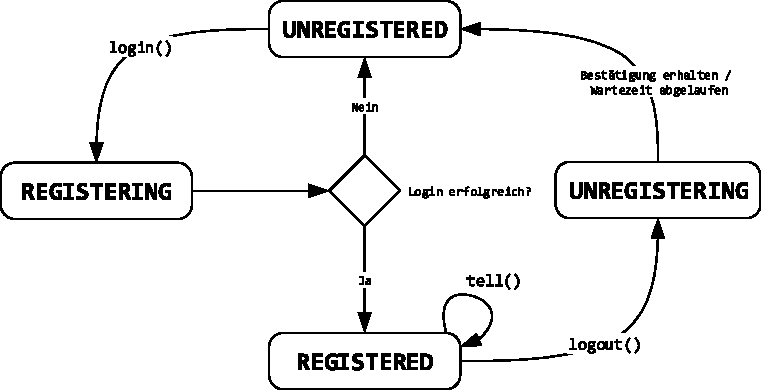
\includegraphics[scale=1]{img/DaKoZustand.pdf}
		\caption{Zustände in der Chat-Anwendung}
		\label{fig:dakoZustand}
	\end{center}
\end{figure}

\noindent Durch den Aufruf der \texttt{login()}-Methode wechselt der Client zunächst in den Zustand \texttt{REGISTERING}. Bestätigt der Server die korrekte Anmeldung, so wechselt der Client in den Zustand \texttt{REGISTERED}. Das Senden von Nachrichten erfolgt mittels \texttt{tell()} und ändert dabei nicht den Zustand des Clients. Die Abmeldung wird durch die Methode \texttt{logout()} initiiert, woraufhin sich der Client im Zustand \texttt{UNREGISTERING} befindet. Wird die Abmeldung vom Server bestätigt bzw. erreicht die Bestätigung den Client nicht innerhalb einer festgelegten Zeitspanne, so wird angenommen, dass die Verbindung geschlossen werden kann und der Client wechselt in den Zustand \texttt{UNREGISTERED}.\\

\noindent Jeder Methodenaufruf generiert dabei eine \texttt{ChatPDU} mit einer Anfrage der zugehörigen Aktion. Beispielsweise wird bei der Anmeldung der PDU-Typ \texttt{LOGIN\_REQUEST} und beim Versand einer Nachricht der Typ \texttt{MESSAGE\_REQUEST} verwendet. Die Verarbeitung der Anfrage ist abhängig von der Implementierung des Servers. Die einfache Implementierung (\texttt{Simple}) benachrichtigt alle angemeldeten Clients über das eingetretene Ereignis und antwortet dem anfragenden Client umgehend. Die komplexe Implementierung (\texttt{Advanced}) sieht vor, dass alle versendeten Events zunächst bestätigt werden müssen, bevor die Antwort an den initiierenden Client versendet wird. Der Ablauf der komplexen Implementierung ist beispielhaft für den Anmeldevorgang in Abbildung \ref{fig:dakoLogin} dargestellt.
\medskip
\begin{figure}[ht] 
	\begin{center}
		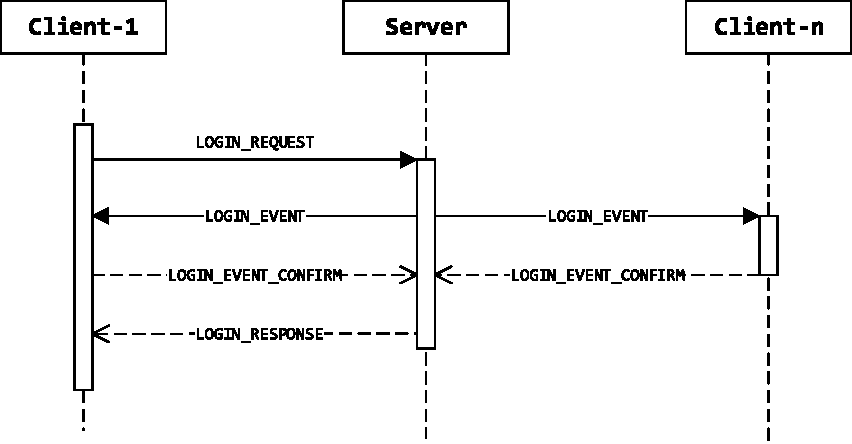
\includegraphics[scale=1]{img/DaKoLogin.pdf}
		\caption{Ablauf des Login-Vorgangs (AdvancedChat)}
		\label{fig:dakoLogin}
	\end{center}
\end{figure}

\noindent Neben den Anfragen, die als \texttt{REQUESTS} versendet werden, können die PDUs des Chat-Protokolls von den Typen \texttt{EVENT} für neue Ereignisse, \texttt{EVENT\_CONFIRM} zur Bestätigung eines Ereignisses und \texttt{RESPONSE} zur Bestätigung der Anfrage sein. Anfragen und Ereignisbestätigungen werden ausschließlich von einem Client verwendet, wohingegen ein Server lediglich über neue Ereignisse informiert und Anfragen bestätigt. Da die Protokollmechanismen genutzt werden sollen, um die \glqq Programmierung von Kommunikationsanwendungen [...] zu erlernen und Erfahrungen mit Transportprotokollen zu sammeln\grqq {} \autocite[vgl.][2]{mandl_aufgabenstellung_2017}, müssen diese im WebSocket-Chat unverändert abgebildet werden.\\

\noindent Das Stellen von Anfragen sowie deren Bearbeitung erfolgt nebenläufig durch die Verwendung von \textit{Threads}. Dabei handelt es sich um leichtgewichtige Prozesse innerhalb eines Prozesses, die sich dessen Ressourcen teilen. Da der gemeinsame Zugriff auf die unterliegenden Ressourcen zu unvorhergesehenen Ergebnissen (\textit{Race Conditions}) führen kann, müssen die Threads mittels geeigneter Mechanismen synchronisiert werden. Die Chat-Anwendung verwendet drei Threads pro Verbindung zwischen Server und Client. Der Server stellt für jeden neuen Client einen dedizierten Thread zur Bearbeitung der Anfragen zur Verfügung. Der Client verfügt über zwei Threads, wobei einer für die Bearbeitung der Benutzerinteraktionen zuständig ist und der andere die Nachrichten des Servers annimmt und bearbeitet. Sowohl die Client-, als auch die Serveranwendung werden als eigenständig Prozesse ausgeführt und können unabhängig voneinander auf verschiedene Hosts verteilt werden. Der WebSocket-Chat soll die Anwendungsteile ebenfalls trennen, wobei die Clientanwendung im Browser und die Serveranwendung auf einem Webserver ausgeführt wird. Der Teil des Clients wird bei einer Webanwendung ebenfalls durch den Webserver ausgeliefert. Durch die Verwendung der Java WebSocket-API wird die Verwaltung der Threads von der spezifischen Implementierung übernommen und kann daher nur eingeschränkt angepasst werden. \\

\noindent Die Übertragung der Protokollnachrichten erfolgt synchron durch die kontinuierliche Übertragung von Objektströmen. Eine zu übermittelnde \texttt{ChatPDU} wird zunächst serialisiert und anschließend in den Puffer des TCP-Sockets übertragen. Für die Serialisierung implementiert die Klasse das Interface \texttt{Serializable}. Überschreitet die Größe der Nachricht den reservierten Speicherplatz des Puffers nicht, so kann der aktive Thread im Anschluss weitere Aufgaben bearbeiten. Im Gegensatz zum nachrichten-basierten WebSocket-Protokoll erfolgt die Übertragung mittels TCP-Sockets \textit{stream-basiert}. Dabei werden die Daten in einem kontinuierlichen Fluss übertragen, dessen Ende vorab nicht ersichtlich ist. Aufgrund der Unterschiede im Aufbau der Protokolle sind nicht alle Eigenschaften der Übertragung von Protokollnachrichten der bestehenden Chat-Anwendung abbildbar. Da jedoch im WebSocket-Chat ebenfalls \texttt{ChatPDUs} übertragen werden sollen, müssen diese entsprechend vor der Übertragung transfomiert werden.

\subsection{Anforderungen an WebSocket-Chat}
Die gewonnenen Erkenntnisse aus der Analyse der bestehenden Chat-Anwendung sollen im Folgenden dazu verwendet werden, die Anforderungen an den WebSocket-Chat zu spezifieren. Eine Anforderungsspezifikation entspricht einer systematisch dargestellten Sammlung von Anforderungen an ein System \autocite[43]{pohl_basiswissen_2009}. Eine Anforderung ist im IEEE Standard 620.16-1990 definiert als \glqq Eine Bedingung oder Fähigkeit, die ein System oder eine Komponente erfüllen oder besitzen muss, um einen Vertrag, einen Standard, eine Spezifikation oder anderweitig formal vorgeschriebene Dokumente zu erfüllen.\grqq{} Dabei wird zwischen funktionalen und nicht-funktionalen Anforderungen unterschieden. Funktionale Anforderungen beziehen sich auf ein erwartetes Ergebnis des Verhaltens einer bereitgestellten Funktion des Systems wohingegen nicht-funktionale Anforderungen an Qualitätsmerkmale des Systems gestellt werden \autocite[16]{pohl_basiswissen_2009}. Diese Qualitätsanforderungen können beispielsweise die Geschwindigkeit oder Verfügbarkeit eines Systems betreffen. Die ermittelten Anforderungen dienen als Basis für den Entwurf des Systems sowie die anschließende Implementierung. Des weiteren werden aus ihnen Testfälle abgeleitet, um die Einhaltung der Systemanforderungen zu überprüfen. 

\subsubsection{Funktionale Anforderungen}
Durch die Analyse der Funktionen der bestehenden Chat-Anwendung wurde eine Vielzahl von Anforderungen an den WebSocket-Chat ermittelt. Im Folgenden werden diese zusammengefasst und in die zugehörigen Bereiche eingeteilt.
\subsubsection*{System und Systemkontext}
Die Chat-Anwendung ist aufgeteilt in Server-, Client- und Benchmarking-Teil. Jeder Teil ist in einem eigenen Prozess ausführbar und kann auf verschiedenen Hostsystemen lokalisiert sein. Der WebSocket-Chat sollte diese Aufteilung weiterhin beibehalten, kann jedoch die Server- und Clientanwendung in einer Einheit bereitstellen. Der Benchmark-Client muss weiterhin als eigenständige Einheit verfügbar sein, um Leistungsmessungen in verschiedenen Szenarien zu ermöglichen. Die Serveranwendung soll in Java 8 durch die Java\texttrademark{} API for WebSocket realisiert werden, wohingegen die Clientanwendung in TypeScript unter Verwendung des Front-End-Webapplikationsframeworks Angular 4 entwickelt wird. Der Benchmark-Client soll als unabhängige Konsolenanwendung in Java 8 implementiert werden und die bisherigen Auswertungsmöglichkeiten bereitstellen.\\

\noindent Die Kommunikation zwischen den Anwendungsteilen muss auf dem WebSocket-Protokoll basieren. Dabei müssen die in Kapitel \ref{sec:WebSocketProtokoll} und Kapitel \ref{sec:WebSocketAPI} beschriebenen Vorgehensweisen und Standards eingehalten werden. Eine WebSocket-Verbindung zwischen Server und Client muss immer über den HTTP Handshake hergestellt werden. Bei den Leistungsmessungen kann gemäß der Spezifikation auf diesen verzichtet werden, da der Benchmark-Client nicht innerhalb eines Browsers ausgeführt wird. \\

\noindent Die Protokollnachrichten, die zwischen den Kommunikationsendpunkten ausgetauscht werden, müssen den Vorgaben der \texttt{ChatPDUs} entsprechen. Dabei sind die Attribute und Methoden vollständig zu übernehmen. Abbildung \ref{fig:chatPDU} bietet einen Überblick über die wichtigsten Elemente der \texttt{ChatPDU}-Klasse. Zur Verbesserung der Lesbarkeit wurde auf \textit{Getter}- und \textit{Setter-}Methoden sowie auf die Parameter der statischen Methoden in der Darstellung verzichtet. Alle statischen Operationen dienen der Erzeugung einer \texttt{ChatPDU} eines bestimmten PDU-Typs. Es werden nur die Attribute mit entsprechenden Werten versehen, die im jeweiligen PDU-Typ benötigt werden. So soll beispielsweise keine Liste aller angemeldeten Clients beim Senden einer neuen Chat-Nachricht (\texttt{MESSAGE\_EVENT}) hinterlegt werden. Die verschiedenen Zustände, die eine \texttt{ChatPDU} annehmen kann, sind in der Enumeration \texttt{PduType} definiert. Der Status des Clients wird der Enumeration \texttt{ClientConversationStatus} entnommen und kann die in Abbildung \ref{fig:dakoZustand} dargestellten Werte annehmen. 
\medskip
\begin{figure}[ht] 
	\begin{center}
		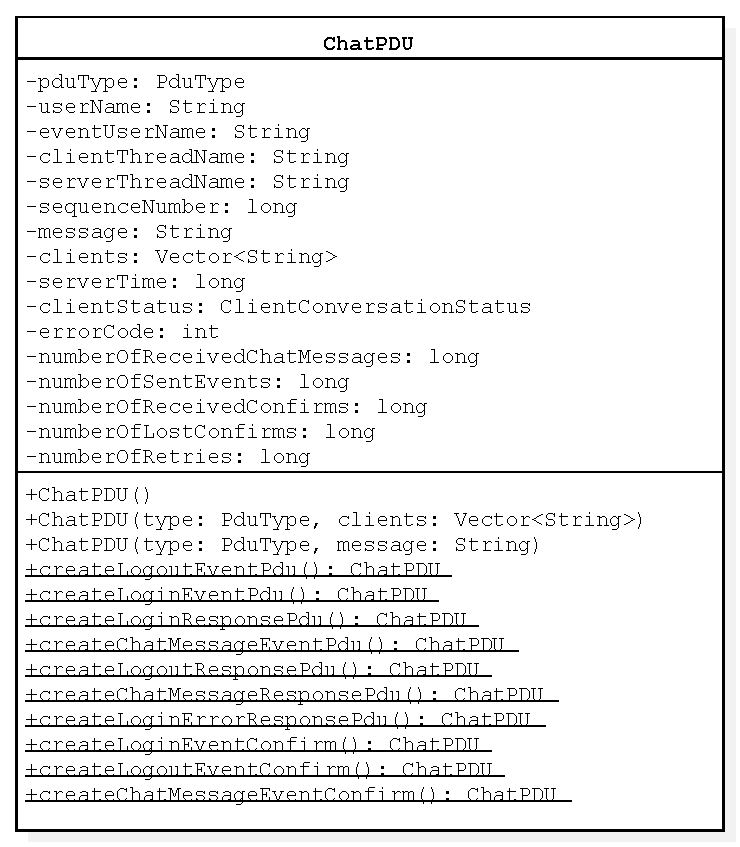
\includegraphics[scale=0.7]{img/ChatPDU.pdf}
		\caption{Aufbau einer ChatPDU}
		\label{fig:chatPDU}
	\end{center}
\end{figure}

\noindent Die bestehende Chat-Anwendung verfügt über zwei unterschiedliche Implementierungsformen. In der einfachen Variante (\texttt{SimpleChat}) wird die Antwort des Servers auf die Anfrage eines Clients umgehend versendet. Die komplexe Variante (\texttt{AdvancedChat}) erwartet zunächst eine Bestätigung des Ereignisses durch alle aktiven Clients, bevor die Antwort an den Initiator versendet wird. Ein Client gilt als aktiv, wenn er sich nicht im Zustand \texttt{UNREGISTERED} befindet. Beide Implementierungsformen dienen als wichtiges didaktisches Mittel und müssen daher im WebSocket-Chat abgebildet werden. Es soll möglich sein, zwischen beiden Implementierungsformen zu wechseln.

\subsubsection*{Funktionen des Server}
Der Server stellt die zentrale Komponente der WebSocket-Chatanwendung dar. Er muss die Nachrichten der Clients empfangen und verarbeiten können. Dazu muss der Server in der Lage sein, Informationen zu jedem verbundenen Clients zu speichern und entsprechende Anfragen dem Initiator zuzuordnen. Der Server muss daher jederzeit den Zustand und die Adresse aller verbundenen Clients abrufen können. Treffen Anfragen eines Clients ein, die eine Statusänderung zur Folge haben, so muss der Server den gespeicherten Zustand des Clients umgehend ändern können. Die Benutzernamen innerhalb des WebSocket-Chats müssen eindeutig sein. Verwendet ein Client beim Verbindungsaufbau einen bereits existierenden Namen, so muss der Server die Anmeldung verweigern und einen entsprechenden Fehlercode in seiner Antwort hinterlegen. Chat-Nachrichten dürfen ausschließlich von Clients gesendet werden, die sich im Status \texttt{REGISTERED} befinden. Eintreffende Chat-Nachrichten von Clients mit einem anderen Status müssen verworfen werden. Der Verbindungsabbau wird clientseitig gestartet und muss vom Server bestätigt werden. Befindet sich der Client im Status \texttt{UNREGISTERED}, kann eine neue Verbindung aufgebaut werden. Bei der Verwendung der \texttt{Simple-Chat}-Implementierung muss der Server bei einer eintreffenden Anfrage alle aktiven Clients über das Ereignis informieren und anschließend eine Bestätigung an den initiierenden Client senden. Die komplexere \texttt{AdvancedChat}-Implementierung verlangt, dass der Server nach der Benachrichtigung aller aktiven Clients zunächst auf deren Empfangsbestätigung wartet, bevor die Antwort an den Initiator erfolgt.

\subsubsection*{Funktionen des Clients}
Die Clientanwendung soll einem Anwender ermöglichen, am WebSocket-Chat teilzunehmen. Dazu muss die Clientanwendung über eine grafische Oberfläche verfügen, über welche der Anwender sich anmelden, Nachrichten versenden und sich abmelden kann. Für die Anmeldung muss der Anwender einen Benutzernamen eingeben können. Existiert dieser Name bereits in der Chatanwendung, so wird dem Anwender die Anmeldung verweigert und er wird darüber benachrichtigt. Der Anwender muss anschließend in der Lage sein, die Anmeldung mit einem neuen Benutzernamen zu wiederholen. Nach einer erfolgreichen Anmeldung müssen Anwender untereinander Nachrichten austauschen können. Sie sollen dabei jederzeit die Benutzernamen aller angemeldeten Anwender sehen können. Alle Nachrichten, die seit dem Zeitpunkt der Anmeldung eines Anwender gesendet wurden, sollen für diesen einsehbar sein. Die Abmeldung von der Chat-Anwendung muss über eine Schaltfläche möglich sein. \\

\noindent Beim Start der Anwendung befindet sich der Client im Zustand \texttt{UNREGISTERED}. Ausschließlich Clients mit diesem Status sollen eine Anmeldeaufforderung angezeigt bekommen. Durch die Anmeldung wechselt der Client in den Zustand \texttt{REGISTERING} und insofern diese erfolgreich ist in \texttt{REGISTERED}. Durch diesen Status erhält der Anwender Zugriff auf den Chat. Meldet sich der Anwender ab, so wechselt der Client in den Zustand \texttt{UNREGISTERING} und wartet auf die Bestätigung durch den Server. Beim Erhalt dieser Bestätigung oder nach einer vordefinierten Wartezeit wechselt der Client in den Status \texttt{UNREGISTERED}. Der Client muss in der Lage sein, den eigenen Zustand zu speichern und zu ändern. Die Änderung wird entweder durch eine Aktion des Anwenders ausgelöst, oder durch eine Antwort des Servers.   

\subsubsection*{Funktionen des Benchmark-Clients}
Der Benchmark-Client nutzt die Funktionsweise der Clientanwendung. Für die Leistungsmessung soll er eine große Anzahl simultan agierender Clients bereitstellen. Eine grafische Oberfläche wird dazu nicht benötigt. Der Benchmark-Client muss in der Lage sein, die Messergebnisse aus Abbildung \ref{fig:dakoBenchClientUI} zu erheben. Die Eingabeparameter des bestehenden Benchmark-Clients müssen als Konsolenparameter abgebildet werden. Folgende Parameter müssen konfigurierbar sein:
\begin{itemize}
\singlespacing{
\item Implementierungsart (Simple/Advanced)
\item Serveradresse (IP-Adresse oder Hostname)
\item Anzahl der Clients
\item Anzahl der Nachrichten pro Client
\item Länge einer Nachricht in Byte
\item Wartezeit eines Clients vor dem Senden der nächsten Nachricht
}
\end{itemize}


\subsubsection{Nicht-funktionale Anforderungen}
Betrifft eine Anforderung mehrere oder alle funktionalen Anforderungen oder überschneidet sie, so handelt es sich um eine nicht-funktionale Anforderung \autocite[109]{balzert_lehrbuch_2011}. Für viele Anforderungen dieser Art lassen sich Qualitätskriterien definieren. Einer Studie von Forschern der University of Technology Sydney zufolge, sind die am häufigsten berücksichtigten Qualitätsmerkmale Leistung (performance) (89\%), Zuverlässigkeit (reliability) (68\%), Benutzbarkeit (usability) (62\%), Sicherheit (security) (60\%) und Wartbarkeit (maintainability) (55\%) \autocite[314]{mairiza_investigation_2010}. Die nicht-funktionalen Anforderungen an den WebSocket-Chat werden im folgenden Abschnitt diesen Kategorien zugeteilt. Da die zu entwickelnde Anwendung im Rahmen einer Lehrveranstaltung zu didaktischen Zwecken eingesetzt werden soll, werden Sicherheitsaspekte jedoch nicht betrachtet.
\subsubsection*{Leistung}
Anforderungen bezüglich der Leistung einer Anwendung spezifieren die Fähigkeit der Software eine angemessene Geschwindigkeit im Verhältnis zu den eingesetzten Ressourcen zu gewährleisten \autocite[315]{mairiza_investigation_2010}. So soll die Anwendung beim Senden einer Nachricht nicht auf eine Bestätigung des Empfängers warten, sondern weitere Aufgaben bearbeiten können. Die Messergebnisse des Leistungstests des WebSocket-Chats sollen maximal um das 2,5-Fache über den Werten der bestehenden Chat-Anwendung liegen. Dieser Faktor wird gewählt, da Forschungsergebnisse zeigen, dass die Kommunikation über WebSockets im Vergleich zu TCP einen Overhead von 150-250\% hat \autocite[1007]{skvorc_performance_2014}.

\subsubsection*{Zuverlässigkeit}
Anforderungen bezüglich der Zuverlässigkeit einer Anwendung spezifieren die Fähigkeit der Software fehlerfrei ein definiertes Leistungsniveau unter regulären Bedingungen für einen vorgegebenen Zeitraum einzuhalten \autocite[315]{mairiza_investigation_2010}. Der WebSocket-Chat soll im Falle einer abgebrochenen Clientverbindung weiterhin für alle anderen Clients funktionieren. Der Client, dessen Verbindung fehlerhaft beendet wurde, wird aus der aktiven Chat-Sitzung entfernt und soll sich anschließend erneut anmelden können.

\subsubsection*{Benutzbarkeit}
Anforderungen bezüglich der Benutzbarkeit einer Anwendung betreffen die Interaktionen eines Benutzers mit dem System. Dies betrifft auch die Erlernbarkeit und Bedienbarkeit des Systems \autocite[315]{mairiza_investigation_2010}. Der WebSocket-Chatclient soll durch die Verwendung von Angular 4 als \textit{Single-Page-Webanwendung} entwickelt werden. Eine solche Webanwendung besteht aus einer einzigen HTML-Seite, deren Inhalte dynamisch nachgeladen werden und somit die Notwendigkeit von Unterseiten entfällt. Des weiteren soll durch eine moderne Benutzeroberfläche sichergestellt werden, dass Benutzer intuitiv im System navigieren können. Die passende dynamische Skalierung für mobile Endgeräte soll ebenfalls gewährleistet sein.

\subsubsection*{Wartbarkeit}
Anforderungen bezüglich der Wartbarkeit einer Anwendung spezifieren, in welchem Maße der Quellcode einer Software verständlich, korrigierbar und verbesserbar ist \autocite[315]{mairiza_investigation_2010}. Der Quellcode des WebSocket-Chats ist in ausreichendem Maß zu dokumentieren. Es soll sichergestellt werden, dass Studenten des Fachbereichs (Wirtschafts-)Informatik nach einer angemessenen Einarbeitungszeit in der Lage sind, den Quellcode zu verstehen und zu erweitern. Da die Erweiterung der internen Abläufe im Fokus der Lehrveranstaltung steht, sollen die Klassen der jeweiligen Implementierungsform (\texttt{Simple} und \texttt{Advanced}) getrennt voneinander realisiert werden.
\subsection{Entwurf und Implementierung des WebSocket-Chats}
Der \textit{Entwurf} ist der Prozess, in welchem die Architektur, Komponenten, Schnittstellen sowie weitere Eigenschaften eines Systems hinsichtlich spezifizierter Anforderungen definiert werden \autocite[25]{insitute_of_electrical_and_electronics_engineers_ieee_1990}. Der Entwurf wird für die Implementierung der Anwendung bentötigt und dokumentiert anhand formeller Darstellungen die Architektur der Software. \\

\noindent Die \textit{Implementierung} beschreibt den Prozess, in welchem der Entwurf in die Komponenten einer Software umgesetzt wird \autocite[38]{insitute_of_electrical_and_electronics_engineers_ieee_1990}. Dabei werden die abstrakten Modelle durch die Verwendung geeigneter Datenstrukturen und Algorithmen in eine konkrete Programmiersprache umgesetzt. Die Entscheidungen, die während der Implementierungsphase getroffen werden, müssen dokumentiert werden.
\subsubsection{Entwurf}
Neben dem Entwurf der internen Software-Architektur muss auch die physische Architektur und die Distribution auf der technischen Infrastruktur beachtet werden \autocite[6]{balzert_lehrbuch_2011}. Der zu entwickelnde WebSocket-Chat wird nicht produktiv eingesetzt. Das bedeutet, dass keine Archivierung von Nachrichten oder eine anderweitige Persistierung von Zuständen der Anwendung erfolgt. Die Software-Architektur des WebSocket-Chats kann daher vereinfacht werden. Die Serveranwendung besteht lediglich aus einem funktionalen Teil, der die Anfragen der Clients bearbeitet. Die Clientanwendung im Browser des Anwenders verfügt zusätzlich noch über einen Darstellungsteil in Form von HTML-Seiten. Der Anwendungsteil zur Durchführung der Lasttests soll als Konsolenanwendung ohne grafische Oberfläche zur Verfügung stehen.
Der WebSocket-Chat wird als Client-Server-System entworfen. Die einzelnen Anwendungsteile lassen sich dabei auf verschiedenen Hostsystemen ausführen. Als Webanwendung besteht zudem die Möglichkeit, die Clientanwendung durch den Webserver bereitstellen zu lassen, der auch die Serveranwendung ausführt. Die URI des WebSocket-Serverendpunkts wird in diesem Fall relativ zum Kontextpfad der Clientanwendung angegeben. \\

\medskip
\begin{figure}[ht] 
	\begin{center}
		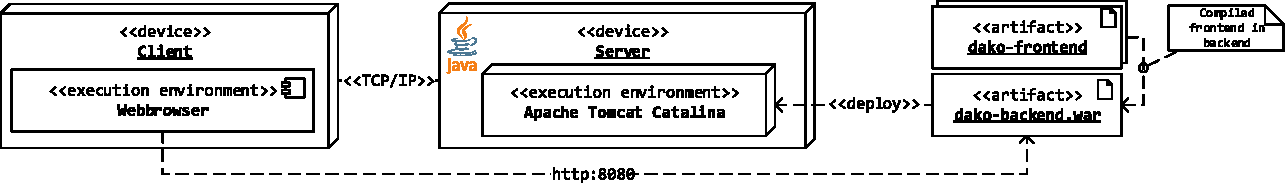
\includegraphics[scale=0.7]{img/vtfinb.pdf}
		\caption{Bereitstellung von Front-und Back-End durch Tomcat Catalina}
		\label{fig:Verteilung1}
	\end{center}
\end{figure}

\noindent Diese Flexibilität wird durch den Einsatz von Java und dem TypeScript-Framework Angular 4 gewährleistet. Die Serveranwendung wird als \textit{Web Application Archive} (WAR) Servlet von einem Webserver bereitgestellt, der die Spezifikation für Java Servlets implementiert und die Java WebSockets-API unterstützt. Der Servlet-Container \textit{Catalina} des \textit{Apache Tomcat} stellt diese Funktionalitäten ab Version 7.0.56 zur Verfügung.\\

\medskip
\begin{figure}[ht] 
	\begin{center}
		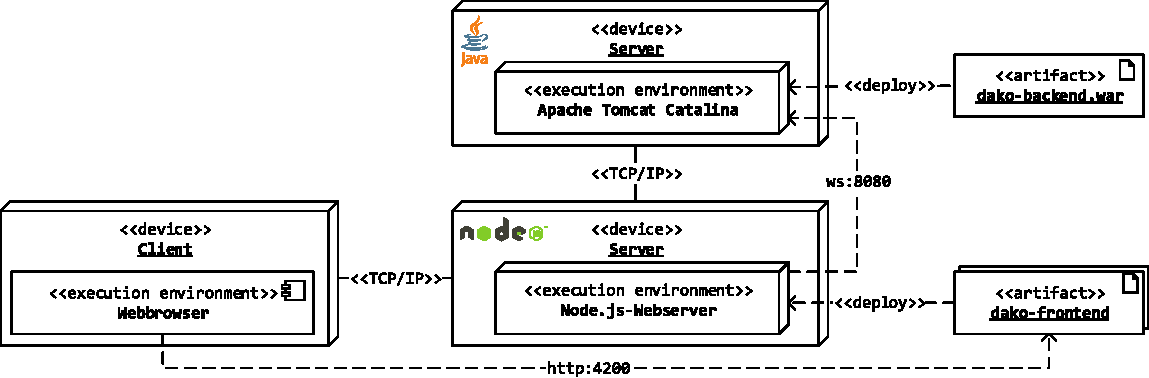
\includegraphics[scale=0.8]{img/vtfohneb.pdf}
		\caption{Bereitstellung des Front-Ends durch Node.js-Webserver}
		\label{fig:Verteilung2}
	\end{center}
\end{figure}

\noindent Der Einsatz von Angular 4 ermöglicht die dedizierte Bereitstellung des kompilierten Front-Ends auf einem \textit{Node.js}-Webserver. Node.js ist ein JavaScript Framework, das auf der Chrome V8 JavaScript Engine basiert und die Entwicklung von serverseitigen JavaScript-Anwendungen ermöglicht \autocite{node_js_foundation_node.js_2018}. Da Client- und Serveranwendung auf dedizierten Hostsystemen ausgeführt werden, muss der Clientanwendung die vollständige URI des Serverendpunkts bekannt sein.\\

\noindent Da der WebSocket-Chatserver ohne grafische Benutzeroberfläche implementiert werden soll und die zusätzlichen Klassen der TCP-Verbindungssteuerung entfallen, reduziert sich der Umfang in den Packages deutlich. Ein detailliertes Klassendiagramm des WebSocket-Chatservers ist in den Abbildungen \ref{fig:kdcommon} und \ref{fig:kdserver} im Anhang zu finden. Der WebSocket-Benchmark-Client verfügt ebenfalls über das Package \texttt{edu.hm.dako.chat.common} und dessen Inhalt. Auf die formelle Darstellung der \texttt{Main}-Klasse wurde verzichtet. Das Klassendiagramm des WebSocket-Benchmark-Clients ist in Abbildung \ref{fig:kdbench} dargestellt. \\

\noindent Die Architektur des WebSocket-Chatclients wird durch die Verwendung des Angular Frameworks um zusätzliche Elemente erweitert, die in Java Anwendungen nicht zu finden sind. Dabei handelt es sich um Komponenten (\textit{Components}) mit einem Anzeigebereich (\textit{View}) und \textit{Services}. Jede Angular Anwendung setzt sich aus verschiedenen Komponenten eines bestimmten Aufgabenbereichs zusammen. Sie sind hierarchisch aufgebaut, wobei alle Komponenten einer Hauptkomponente (\textit{Root Component}) untergeordnet sind. Der Anzeigebereich einer Komponente dient der Darstellung eines HTML-\textit{Templates}, mit welchem der Benutzer interagieren kann \autocite[66]{woiwode_angular_2017}. Services sind Klassen, die ihre Funktionen für andere Klassen bereitstellen. Sie enthalten mehrfach verwendbaren Code und werden über das Entwurfsmuster \textit{Dependency Injection} (DI) bereitgestellt \autocite[117]{woiwode_angular_2017}. DI folgt dem Prinzip der \textit{Inversion of Control} (IoC), welches besagt, dass die Erzeugung einer Abhängigkeit nicht von dem abhängigen Objekt durchgeführt wird, sondern alle Abhängigkeiten an einem zentralen Ort (DI-Container) verwaltet werden. Der Aufbau des WebSocket-Chatclients ist in Abbildung \ref{fig:kdClient} im Anhang dargestellt. Die Klassen des \textit{common}-Packages sind nicht enthalten, da ihre Darstellung zu der in Abbildung \ref{fig:kdcommon} identisch ist.

\subsubsection{Implementierung}
Die Implementierung aller Java-Module wird in der Entwicklungsumgebung \textit{Eclipse Java EE IDE for Web Developers} in Version Oxygen.2 Release (4.7.2) durchgeführt. Die installierte Version von Java ist 1.8.0\_144. Zur Verwaltung der Abhängigkeiten wird Apache Maven 3.5.0 eingesetzt. Die Entwicklung des WebSocket-Chatclients erfolgt in \textit{Visual Studio Code} Version 1.18 und TypeScript 2.6.2. Für die Nutzung des Angular 4 Frameworks wird die Paketverwaltung \textit{npm} in Version 3.10.10 eingesetzt. Die Entwicklung wird auf dem Betriebssystem \textit{macOS High Sierra} 10.13.3 durchgeführt. Die Versionierung der Codebase erfolgt durch \textit{git} unter Verwendung der gleichnamigen Plattform von \textit{Github, Inc}. \\

\noindent Zur Umsetzung der Architektur des WebSocket-Chatservers wird ein Maven-Projekt verwendet um alle benötigten Bibliotheken bereitzustellen. Neben den Bibliotheken, welche aus der bestehenden Anwendung übernommen wurden, wird die Java WebSocket-API sowie Bibliotheken zur Transformation von Java Objekten in das \textit{JSON} Format benötigt. Dieses dient der leichtgewichtigen, textuellen Repräsentation von Objekten in einer lesbaren Form. Die \texttt{ChatPDUs} werden in diesem Format zwischen den Endpunkten übertragen.\medskip

\begin{lstlisting}[frame=single, language=Java, caption=AdvancedWebSocketServer Annotation,label=lst:wsServerImpl]
	@ServerEndpoint(value = "/advancedchat", encoders = { ChatPDUEncoder.class }, decoders = { ChatPDUDecoder.class })
	public class AdvancedWebSocketServer extends AbstractWebSocketServer { ... }
\end{lstlisting}

\noindent Durch die Deklaration der Encoder- und Decoder-Klassen des Serverendpunkts erfolgt die Umwandlung der \texttt{ChatPDUs} in JSON-Objekte automatisch anhand des Vorgehens, welches in den jeweiligen Methoden definiert wurde. Die \texttt{@OnClose}-Methode muss speziell für den Fall angepasst werden, dass Clients die Verbindung durch das Beenden des Browsers oder das Verlassen der Seite schließen. Der Client wird bei Bedarf aus noch vorhandenen Wartelisten und der Liste der angemeldeten Clients entfernt, da jeder weitere Versuch eine Nachricht an diesen Client zu senden mit einer Exception (\textit{broken pipe}) abgebrochen wird.\medskip

\begin{lstlisting}[frame=single, language=Java, caption=Senden einer ChatPDU label=lst:wsServerPDU]
	@Override
	public void sendPduToClient(ClientListEntry client, ChatPDU pdu) {
		try {
			Session session = client.getSession();
			session.getBasicRemote().sendObject(pdu);
		} catch (IOException | EncodeException e) {
		log.error(e.getMessage());
		}
	}
\end{lstlisting}

\noindent Das Senden einer \texttt{ChatPDU} erfolgt über die zugehörige \texttt{Session} eines Clients. Die Übertragung findet synchron an das \texttt{BasicRemote}-Objekt statt, da die asynchrone Alternative bei Nachrichten von geringer Größe keinen Vorteil bietet und die zusätzliche Verwaltung von Future-Objekten oder Callback-Methoden die Komplexität erhöht. Da zwischen den verschiedenen Implementierungsformen eine Trennung erfolgen soll, werden zwei Endpunkte auf unterschiedlichen URIs\footnote{\texttt{/simplechat} und \texttt{/advancedchat}} bereitgestellt. Die Wahl der zu verwendenden Implementierung erfolgt durch die Clientanwendung. \\

\noindent Die Realisierung des Benchmark-Clients setzt die Verwendung einer Bibliothek voraus, welche die Java WebSocket-API implementiert. Dazu wird die Referenzimplementierung \textit{Project Tyrus} der Oracle Corporation eingesetzt. Die Anzahl gleichzeitiger Chat-Clients sollte nebenläufig durch Threads abgebildet werden. Jedoch werden durch die Bibliothek pro Client drei Threads erzeugt, wohingegen in der bestehenden Chatanwendung nur zwei Threads pro Client eingesetzt wurden. Trotz zusätzlicher Synchronisierungsmechanismen war es nicht möglich die Funktionalität zu gewährleisten. Die Leistungsmessung wird aus diesem Grund in mehreren Prozessen ausgeführt. Die Abläufe und Funktionen des bestehenden Benchmark-Clients wurden übernommen.\\

\noindent Die Basisstruktur der Clientanwendung wird mit Hilfe der Angular-CLI erstellt. Für die Nutzung von WebSockets in einer Angular Anwendung wird die Bibliothek \textit{RxJS} benötigt. RxJS ist der JavaScript-Teil des Open-Source-Projekts \textit{ReactiveX.io}, welches den Einsatz von asynchroner Programmierung und des \texttt{Observable} Entwurfsmusters erleichtert. Sie bietet zudem eine Unterstützung für WebSockets. Die API wird durch \texttt{npm install rxjs} dem Projekt hinzugefügt und in dem Service \texttt{websocket.service.ts} hinzugefügt.\medskip

\begin{lstlisting}[frame=single, language=JavaScript, caption=WebSocket-Client: WebSocket-Service, label=lst:wsClientWS]
	import * as Rx from 'rxjs/Rx';

	@Injectable()
	export class WebsocketService {
		private subject: Rx.Subject<MessageEvent>;
		(...)
		private create(url): Rx.Subject<MessageEvent> {
			let webSocket = new WebSocket(url);
			let observable = Rx.Observable.create(
				(obs: Rx.Observer<MessageEvent>) => {
					webSocket.onmessage = obs.next.bind(obs);
					webSocket.onerror = obs.error.bind(obs);
					webSocket.onclose = obs.complete.bind(obs);
					return webSocket.close.bind(webSocket);
				})
			let observer = { next: (data: Object) => {
				if (webSocket.readyState === WebSocket.OPEN) {
					webSocket.send(JSON.stringify(data));
				}
			}
			return Rx.Subject.create(observer, observable);
		} 
		(...)
	}
\end{lstlisting}

\noindent Dieser Service stellt zur Anbindung der bidirektional kommunizierenden WebSockets ein \texttt{Subject}-Objekt bereit, welches Events empfangen und senden kann. Dazu wird sowohl ein \texttt{Observable}, das Events an mehrere Abonnenten senden kann, als auch ein \texttt{Observer} benötigt, der Daten empfängt. Ein Subject kann demnach eingesetzt werden, um eingehende Events von einem WebSocket an die Benutzeroberfläche weiterzuleiten, als auch Daten von diesem an den WebSocket zu übergeben. Dazu wird ein Observable-Objekt erstellt und die Callback-Methoden der abonnierenden Observer an die jeweiligen Event-Handler des WebSockets gebunden. Der Rückgabewert gibt an, das die WebSocket-Verbindung geschlossen wird, wenn der abonnierende Observer sich abmeldet. Der Observer-Teil des Subjects definiert lediglich die Methode \texttt{next}, die dem Observer mitteilt, dass neue Daten vorliegen. In dieser wird zunächst geprüft, ob der zugrundeliegende WebSocket geöffnet ist, bevor die übergebenen Daten in einen JSON-String transformiert und versendet werden. Der WebSocket-Service wird vom Chat-Service verwendet. Dieser wandelt eingehende JSON-Strings in \texttt{ChatPDUs} und übernimmt Funktionen wie Verbindungsaufbau und -abbau.

\noindent Der Ablauf und die Algorithmen des WebSocket-Chats sind im \texttt{AbstractChatClient} bzw. in dessen konkreten Ausprägungen implementiert. Diese werden von den \texttt{Components} App, Chat und Login verwendet. Die \texttt{AppComponent} ist die Hauptkomponente, von der aus die anderen gesteuert werden. Beim Aufruf der Website wird diese zuerst geladen und liefert die \texttt{LoginComponent}, falls der Benutzer noch nicht angemeldet ist. Andernfalls wird die \texttt{ChatComponent} bereitgestellt. \medskip

\begin{lstlisting}[frame=single, caption=WebSocket-Client: AppComponent-View, label=lst:wsClientRoot]
	<div *ngIf="!loggedIn; then thenBlock else elseBlock"></div>
	<ng-template #thenBlock>
		<app-login (clientEvent)="receiveClientService($event)"></app-login>
	</ng-template>
	<ng-template #elseBlock>
		<app-chat [client]="client" (closedEvent)="receiveClosedEvent($event)">
		</app-chat>
	</ng-template>
\end{lstlisting}

\noindent Der Austausch von Objekten zwischen den Komponenten erfolgt entweder durch Übergabe von übergeordneter Komponente (\textit{Parent}) an die aufgerufene Komponente (\textit{Child}) oder durch \texttt{EventEmitter}. Hier empfängt die \texttt{AppComponent} ein Objekt des \texttt{AbstractChatClient}-Services durch einen \texttt{EventEmitter} der \texttt{LoginComponent}. Dieses Event wird erst bei einer erfolgreichen Anmeldung ausgelöst. Der Benutzername des angemeldeten Clients wird dabei im \textit{SessionStorage} gespeichert. Liegt hier ein Wert vor, so gilt der hinterlegte Benutzer als angemeldet und die \texttt{ChatComponent} wird bereitgestellt. Diese empfängt den zu verwendenden Client-Service von der \texttt{AppComponent}. Meldet sich ein Client ab oder läd die Webseite neu, so wird der Benutzername aus dem SessionStorage entfernt und der Client muss sich erneut anmelden. Da im Server entsprechende Vorkehrungen getroffen wurden, kann sich der Client unverzüglich erneut anmelden. Kann der Benutzer nicht angemeldet werden, wird eine Fehlermeldung über dem Login-Bereich ausgegeben. Das Design des WebSocket-Chatclients ist responsive, das bedeutet, dass die Darstellung auf die Größe des Displays des verwendeten Endgeräts angepasst wird. Somit ist der WebSocket-Chat sowohl von einem Smartphone, als auch von einem hochauflösenden Computerbildschirm bedienbar. Dazu wird das CSS-Framework \textit{Semantic UI} eingebunden.
\medskip
\begin{figure}[ht] 
	\begin{center}
		\includegraphics[scale=0.44]{img/LoginErrorView.pdf}
		\caption{WebSocket-Client: Fehlermeldung bei Login}
		\label{fig:errorLoginView}
	\end{center}
\end{figure}

\noindent Im unteren Bereich des Login-Views wird angezeigt, welche Implementierungsform die Client-Services nutzen. Diese Einstellung kann nicht zur Laufzeit verändert, sondern muss in der Konfiguration der Umgebung angepasst werden. Die zugehörigen Konfigurationsdateien lauten \texttt{environment.prod.ts} für die Einstellungen in der Produktivumgebung und \texttt{environment.ts} für Testumgebungen. Als Konfiguration für den Einsatz als eigenständige Anwendung dient die Datei \texttt{environment.ts}. Hier muss neben der Implementierungsform auch die IP-Adresse bzw. der Hostname des WebSocket-Servers hinterlegt werden. Soll der WebSocket-Client hingegen ebenfalls von der Serveranwendung ausgeliefert werden, so wird die Produktivkonfiguration verwendet. Dazu muss die durch den Befehl \texttt{ng build --prod --base-href /NAME\_DES\_JAVA-PROJEKTS/} kompilierte Clientanwendung in den \texttt{webapp}-Ordner des WebSocket-Serversprojekts verschoben werden.

\newpage
\section{Evaluation}\label{sec:Evaluation}
Die Durchführung der Leistungsmessung soll einen Vergleich zwischen der bestehenden Chatanwendung und dem entwickelten WebSocket-Chat ermöglichen. Dazu sollen die Implementierungen der jeweiligen Benchmark-Clients eingesetzt werden. Zur Realisierung einer geeigneten Umgebung wird ein dediziertes Netzwerk verwendet, in welchem die Clients und der Server ausgeführt werden können. Der Aufbau des Netzwerks ist in Abbildung \ref{fig:evalNetwork} dargestellt.
\medskip
\begin{figure}[ht] 
	\begin{center}
		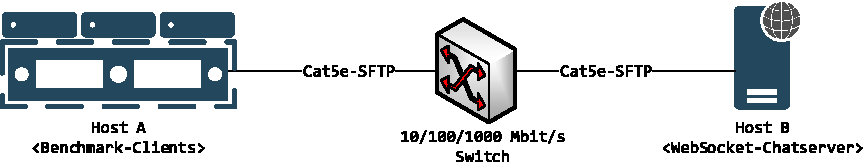
\includegraphics[scale=1]{img/umgebung.pdf}
		\caption{Netzwerk der Test-Konfiguration}
		\label{fig:evalNetwork}
	\end{center}
\end{figure}

\noindent Der WebSocket-Chatserver befindet sich auf einem dedizierten Host, der die Anwendung mittels des Webservers \textit{Apache Tomcat} (Version 9.0.0.M26) bereitstellt. Die Benchmark-Clients werden als virtuelle Maschinen auf einem Hostsystem ausgeführt. Es kommen drei dieser Instanzen zum Einsatz. Die physikalischen Hosts verfügen jeweils über eine 1000 Mbit/s Verbindung. Die technische Konfiguration der Testsysteme ist in Tabelle \ref{tbl:evalEnv} abgebildet. \\

\renewcommand{\arraystretch}{1.5}
\begin{table*}[ht]
	\begin{center}
		\begin{tabular}{|c|>{\centering\arraybackslash}m{7cm}|>{\centering\arraybackslash}m{5cm}|}
			\hline
			 &  \textbf{Benchmark-VM} &  \textbf{WebSocket-Chatserver}  \\ \hline
			\textbf{OS} &  Ubuntu 16.04 LTS &  macOS HighSierra \\ \hline
			\textbf{CPU} &  1 Core &  Intel Core i5-7360U  \\ \hline
			\textbf{RAM} &  4GB &  8GB  \\ \hline
			\textbf{Virtualization} &  VMWare Workstation Pro 12 &  -  \\ \hline
			\textbf{Hypervisor} &  Typ2 (OS: Windows 10 x64, CPU: Intel Core i5-4460, RAM: 16GB) &  -  \\ \hline
		\end{tabular}
		\caption{Konfiguration der Test-Umgebung}\label{tbl:evalEnv}
	\end{center}
\end{table*}
\renewcommand{\arraystretch}{1}
\noindent Die Messungen der bestehenden Anwendung werden in der gleichen Umgebung durchgeführt. Jedoch wird hier nur eine der virtuellen Maschinen für die Clientanwendung eingesetzt. Die IP-Adressen der Systeme werden manuell konfiguriert. Die Serveranwendungen sind über die TCP-Ports 8080 (WebSocket-Chatserver) bzw. 50000 (TCP-Chatserver) erreichbar. 
\subsection{Komplikationen} \label{subsec:EvalKompl}
Die Anwendungen sollten sich lediglich durch die Verwendung des Übertragungsprotokolls unterscheiden, um die Vergleichbarkeit der Messergebnisse zu gewährleisten. Die Simulation mehrerer gleichzeitiger Benutzer soll nebenläufig durch Threads erfolgen. Die zur Realisierung des Benchmark-Clients eingesetzte Bibliothek \textit{Tyrus 1.12} verwendet für jede Verbindung eines WebSocket-Clients drei Threads, wohingegen die ursprüngliche Implementierung die Verwendung von zwei Threads vorsieht. Trotz zusätzlicher Synchronisierungsmechanismen konnte die fehlerfreie Ausführung der WebSocket-Leistungsmessungen nicht gewährleistet werden. Aus diesem Grund wird der WebSocket-Benchmarkclient in mehreren Prozessen gestartet. Der zusätzliche Aufwand zur Verwaltung der Prozesse durch das Betriebssystem wirkt sich negativ auf die Leistung des WebSocket-Chats aus. Durch die Verwendung einer anderen WebSocket-Bibliothek oder eines browserbasierten Benchmarkings könnte eine erhebliche Verbesserung der Messergebnisse erzielt werden. \\

\noindent Die Prozesse der WebSocket-Clients zur Leistungsmessung werden auf die drei virtuellen Maschinen verteilt. Damit diese in möglichst kurzen Zeitabständen starten können, wird deren Ausführung durch zwei Bash-Skripte gesteuert. Das erste Skript trägt die Bezeichnung \texttt{start\_benchmark.sh} und empfängt folgende Werte als Parameter:
\renewcommand{\arraystretch}{1.5}
\begin{table*}[ht]
	\begin{center}
		\begin{tabular}{|>{\centering\arraybackslash}m{4cm}|m{7.5cm}|>{\centering\arraybackslash}m{3cm}|}
			\hline
			  \textbf{Parameter} & \textbf{Beschreibung} & \textbf{Beispiel} \\ \hline
			  Adresse des WebSocket-Servers & Die Angabe muss den verwendeten Port und den Namen der Anwendung enthalten, unter welcher der Endpunkt bereitgestellt wird. & 10.0.0.1:8080/chat \\ \hline
			  Anzahl der Clients pro Host & Im Skript können die IP-Adressen der Systeme hinterlegt werden, die als Hosts für die Benchmark-Clients dienen. Es wird auf jedem Host die übergebene Anzahl Clients gestartet. & 10 (x3 = 30)\\ \hline
			  Anzahl Nachrichten & Die Anzahl der Nachrichten, die pro Client gesendet werden sollen. & 10 \\ \hline
			  Nachrichtenlänge & Die Länge einer Nachricht in Byte. & 10 \\ \hline
			  Denkzeit des Clients & Die Zeit in ms, die ein Client zwischen dem Senden von zwei Nachrichten wartet. & 100 \\ \hline
			  Benutzen des AdvancedChats & Anhand dieser Angabe wird der zu verwendende Implementierungstyp festgelegt. & y oder n\\ \hline
		\end{tabular}
		\caption{Parameter des Benchmark-Skripts}\label{tbl:scriptParams}
	\end{center}
\end{table*}
\renewcommand{\arraystretch}{1}

\noindent Das Skript stellt bei seiner Ausführung eine SSH-Verbindung zu den hinterlegten Hosts her und führt dort das Skript \texttt{run\_client\_benchmark.sh} im Hintergrund aus. Hier findet der Aufruf des Benchmark-Clients statt, welcher ebenfalls als Hintergrund-Prozess gestartet wird. Der jeweils letzte Aufruf blockiert die weitere Ausführung, damit Skript und Benchmark-Prozess zeitgleich enden. Der Benchmark-Client sammelt alle Messwerte und legt sie als JSON-String in einer Textdatei ab. Wurden alle Instanzen des Benchmark-Clients beendet, werden die Resultate der einzelnen Testläufe durch das Startskript gesammelt und von einer Java-Konsolenanwendung ausgewertet. Diese importiert die Informationen aller Clients und ermittelt die statistischen Ergebnisse des gesamten Durchlaufs.

\begin{lstlisting}[frame=single, caption=Resultat eines Benchmark-Clients, label=lst:evalJSONResultat]
	{
		"userName":"Client-Thread-1", "implementation":"Advanced",
		"totalEvents":6, "sendMessages":2,	"loginEvents":2, "logoutEvents":2,
		"chatPduRtt":[28270117128,17249212499],
		"serverTime":[25951704704,17245024235]
	}
\end{lstlisting}

\noindent Die Leistungsmessung der bestehenden Chatanwendung kann jedoch nicht auf mehrere Hosts aufgeteilt werden, da jede Instanz die Benutzernamen der Clients gleich nummeriert. Das System verhindert jedoch die Anmeldung gleichnamiger Benutzer. Aus diesem Grund wird die Leistungsmessung der TCP-Chatanwendung auf nur einer virtuellen Maschine durchgeführt.

\subsection{Leistungsanalyse WebSocket-Chat} \label{subsec:Benchmark}
Die Metrik zur Messung der Leistung des WebSocket-Chats ist die \textit{Round Trip Time} (RTT). Dabei handelt es sich um die Zeit, die zwischen dem Stellen einer Anfrage und dem Eintreffen der zugehörigen Antwort vergeht. Die Zeit, die der Server zur Bearbeitung der Anfrage benötigt, wird als \textit{Server Time} bezeichnet. Die Dauer der reinen Kommunikation errechnet sich aus der Differenz zwischen RTT und Server Time ($ \text{T}_{\text{k}} = \text{RTT}-\text{Server Time} $).
\medskip
\begin{figure}[ht] 
	\begin{center}
		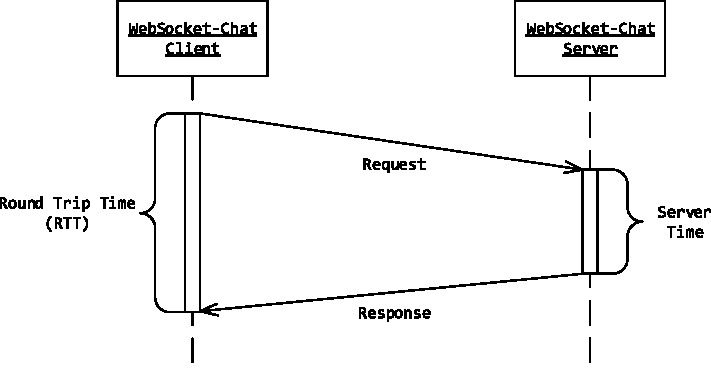
\includegraphics[scale=1.0]{img/rtt.pdf}
		\caption{Metriken der Leistungsmessung des WebSocket-Chats}
		\label{fig:RTT}
	\end{center}
\end{figure}

\noindent Für die Leistungsmessungen wird die Anzahl der aktiven Clients variiert. Jeder Client versendet 10 Nachrichten mit einer Länge von 10 Byte. Die Clients haben eine maximale Denkzeit von 100 ms. Jede Messung wird dabei fünf Mal wiederholt. Die Ergebnisse der Advanced-Benchmarks sind in den Tabellen \ref{tbl:evalWebSocket} und \ref{tbl:evalTCP} zusammengefasst. Insbesondere bei den Zeitmessungen der Round Trip Time und der Serverzeit ist zu erkennen, dass die Messergebnisse des WebSocket-Chats die Werte des TCP-Chats signifikant übersteigen.Die Ursachen dieser Abweichungen sind zahlreich. Zum einen wirken sich die in Abschnitt \ref{subsec:EvalKompl} beschriebenen Unterschiede negativ auf die Leistungsfähigkeit des WebSocket-Chats aus, zum anderen liegen sie in der Verschiedenartigkeit der Protokolle selbst begründet. \\

\begin{figure}[ht] 
	\begin{center}
		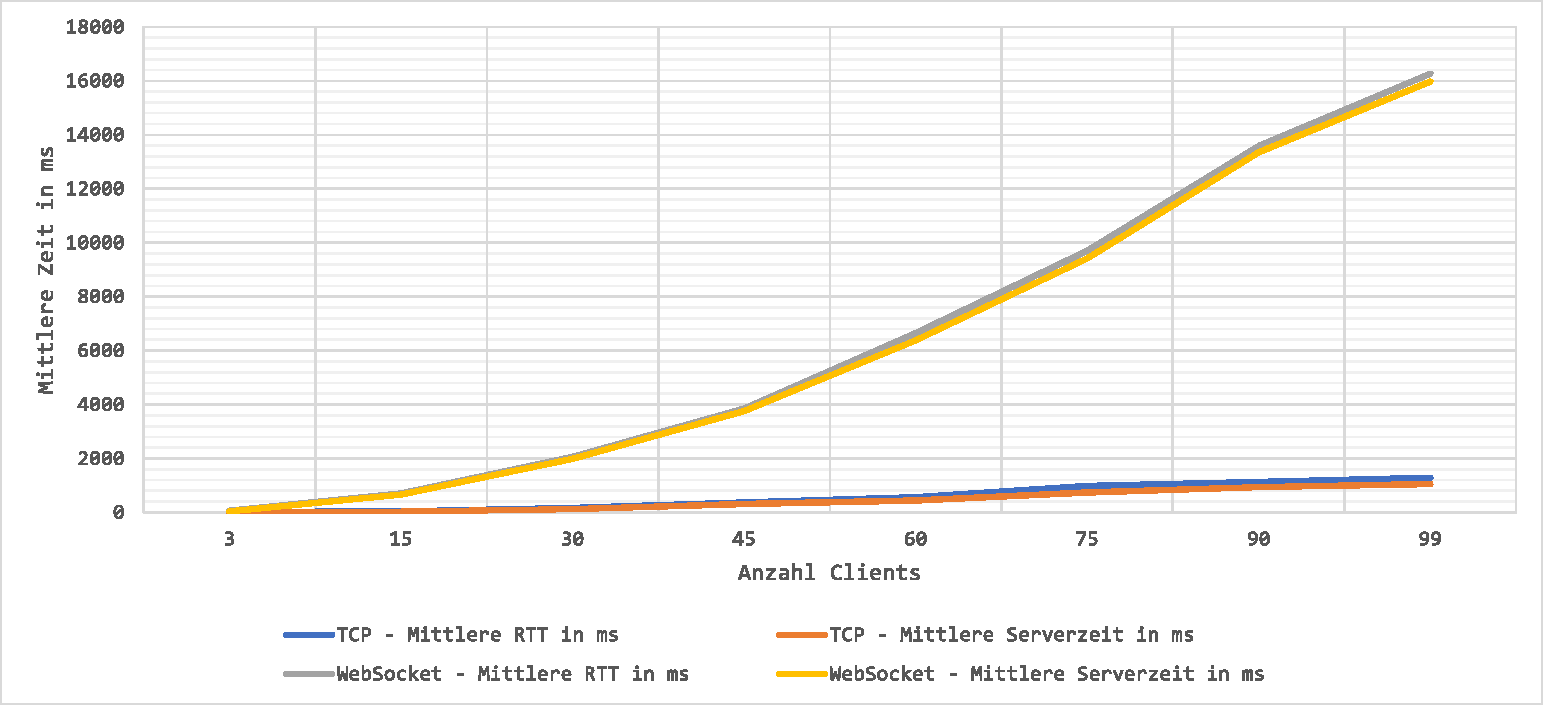
\includegraphics[scale=0.5]{img/benchmark-rttst.pdf}
		\caption{Messergebnisse RTT und Serverzeit}
		\label{fig:evalRttSt}
	\end{center}
\end{figure}
\begin{figure}[ht] 
	\begin{center}
		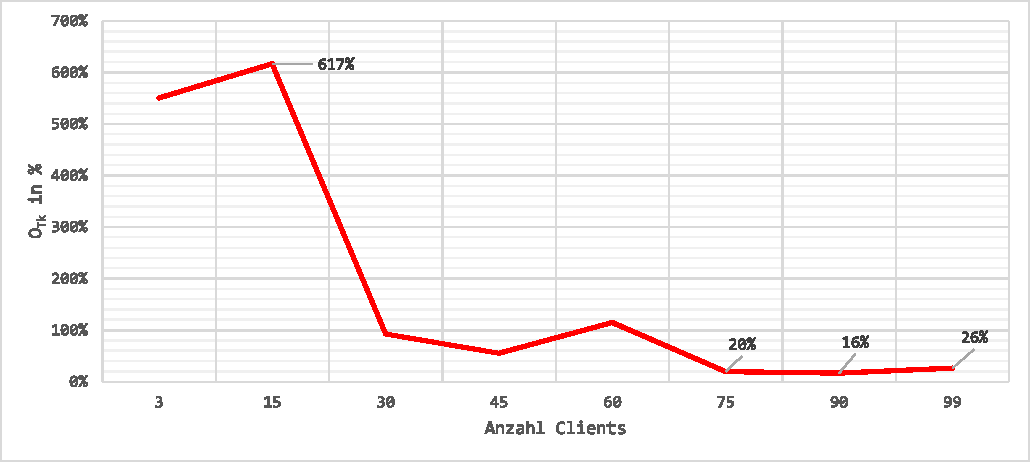
\includegraphics[scale=0.7]{img/benchmark-tk.pdf}
		\caption{WebSocket-Overhead für reine Kommunikationsdauer}
		\label{fig:evalTk}
	\end{center}
\end{figure} 
\noindent Das WebSocket-Protokoll agiert auf einer höheren Schicht des TCP/IP-Referenzmodells und benötigt zusätzliche Zeit und Rechenleistung für die Übertragung von der TCP-Schicht in die eigene Ebene. Zudem verwendet das WebSocket-Protokoll eventgesteuerte Callback-Mechanismen, die zusätzlichen Verwaltungsaufwand auf Anwendungsebene erfordern \autocite[1007]{skvorc_performance_2014}. Der zeitliche Aufwand für die Maskierung clientseitiger Nachrichten kann nicht dediziert erfasst werden und erhöht die erfassten Messwerte ebenfalls. Darüber hinaus könnten auch die Java-Implementierungen der Protokolle ins Gewicht fallen. Das WebSocket-Protokoll wurde erst vor kurzer Zeit entwickelt und die verwendete API ist eine frühe Referenzimplementierung, wohingegen TCP bereits seit Jahrzehnten eingesetzt wird und kontinuierlich optimiert wurde \autocite[1007]{skvorc_performance_2014}. \\

\noindent Auch die Dauer der reinen Kommunikation des WebSocket-Chats übersteigt die des TCP-Chats, jedoch reduziert sich der Overhead (Berechnung anhand Gleichung \ref{eq:Overhead}) mit steigender Anzahl verbundener Clients. \\
\begin{equation}\label{eq:Overhead}
	O_{T_{k}} = \dfrac{T_{k (WebSocket)} - T_{k(TCP)}}{T_{k(TCP)}} \ast 100\%
\end{equation}

\noindent Ausschlaggebend für diese Entwicklung sind die unterschiedlichen Nachrichtengrößen und die Verwendung der Callback-Mechanismen. Die übrigen Faktoren wirken sich erst beim Einsatz mehrerer Clients wesentlich auf die reine Kommunikationszeit aus. Beispielsweise ist der zusätzliche Aufwand für Kontextwechsel bei nur drei Threads sehr gering, bzw. bei nur einem Prozess muss kein Kontextwechsel durchgeführt werden. \\

\noindent Die bestehende Chatanwendung zeigt im direkten Leistungsvergleich einen signifkanten Geschwindigkeitsvorteil. Die Kommunikation über TCP ist leichtgewichtiger und schneller als über WebSockets. Zur besseren Vergleichbarkeit sollten jedoch weitere Anwendungen und Bibliotheken zur Leistungsmessung herangezogen werden. Beispielsweise birgt der Einsatz einer Java WebSocket-Bibliothek, die eine Parallelisierung durch Threading ermöglicht, erhebliches Verbesserungspotential. Zudem sollten sich WebSocket-Leistungsmessungen auf Webtechnologien wie JavaScript oder Typescript fokussieren, da diese den primären Anwendungsfall für einen Client darstellen. 

\newpage
\section{Fazit und Ausblick}
In dieser Arbeit wurde die praktische Einsetzbarkeit von HTML5 WebSockets anhand der Migration der Kommunikationsstruktur einer auf TCP-Sockets basierenden Chatanwendung geprüft. Dazu wurden in Kapitel 2 zunächst die wichtigsten Aspekte der neuen Protokollspezifikation detailliert dargelegt, um daraus die Vorzüge der Technologie gegenüber dem Anfrage/Antwort-Verfahren von HTTP abzuleiten. Durch das WebSocket-Protokoll können Informationen zwischen Server und Client bidirektional ausgetauscht werden, ohne dass der Client eine neue Anfrage initiieren muss. Des weiteren reduziert es den durch Zusatzinformationen verursachten Overhead erheblich, da dieser nach dem erfolgreichem Aufbau einer Verbindung lediglich 2-14 Byte beträgt. Die Implementierung des Protokolls durch die WebSocket-API des W3C und das entsprechende Java-Pendant wurden in Kapitel 3 ausführlich vorgestellt.\\

\noindent Anhand der daraus gewonnenen Erkenntnisse wurde in Kapitel 4 die Überarbeitung der Chatanwendung geplant und durchgeführt. Hierzu wurde zunächst eine Anforderungsanalyse anhand der Funktionalität des Altsystems durchgeführt. Auf dieser Grundlage wurde die Architektur des WebSocket-Chats entworfen und anschließend implementiert. Die entwickelte Anwendung ermöglicht den Austausch von Chatnachrichten für mehrere Benutzer. Die Funktionalität ist dabei für eine Vielzahl verschiedener Endgeräte gewährleistet. In Kapitel 5 werden die Leistung der WebSocket-Chatanwendung und die des Altsystems gegenübergestellt. Die Messergebnisse zeigen, dass der WebSocket-Chat bis zu 13-mal länger für die Bearbeitung einer Anfrage benötigt, als der TCP-Chat bei gleicher Anzahl angemeldeter Benutzer. Diese Werte resultieren zum einen aus der Beziehung zwischen den Protokollen. Das WebSocket-Protokoll agiert auf Anwendungsebene und setzt auf TCP auf. Die Übertragung zwischen den Schichten erfordert zusätzliche Zeit sowie Rechenleistung und führt folglich zu schlechteren Leistungswerten. Zum anderen werden die Ergebnisse jedoch von diversen Komplikationen bei der Umsetzung beeinflusst, die nicht im Zusammenhang mit den verwendeten Protokollen stehen. \\

\noindent Die Technologie der HTML5 WebSockets überzeugt sowohl durch die funktionale, leichtgewichtige Architektur des Protokolls, als auch durch die komfortable Handhabung der zugehörigen APIs. Entwickler moderner Webanwendungen, die Informationen zwischen Server und Client bidirektional austauschen sollen, verfügen dadurch über einen standardisierten Weg zur Umsetzung dieser Anforderung. Die Unterstützung von WebSockets ist inzwischen durch nahezu alle aktuellen Webbrowser und -server gegeben. Dennoch kann aus Leistungsgründen von der Migration bestehender Systeme abgeraten werden, insofern deren Kommunikation auf TCP basiert und innerhalb des eigenen Netzwerks stattfindet. Jedoch werden mit zunehmender Akzeptanz und Verbreitung diverse Erweiterungen und Optimierungen das WebSocket-Protokoll verbessern. Daher sollten weitere Untersuchungen sowohl die Leistungsfähigkeit der unterschiedlichen WebSocket-Bibliotheken einer Programmiersprache, als auch zwischen den verschiedenen Programmiersprachen auf deren Leistungsfähigkeit vergleichen. 

\newpage
\appendix
\pagenumbering{Roman}
\printbibliography
\newpage
\listoffigures
\newpage
\listoftables
\newpage
\lstlistoflistings
\newpage
\section{Anhang}
\begin{figure}[ht] 
	\begin{center}
		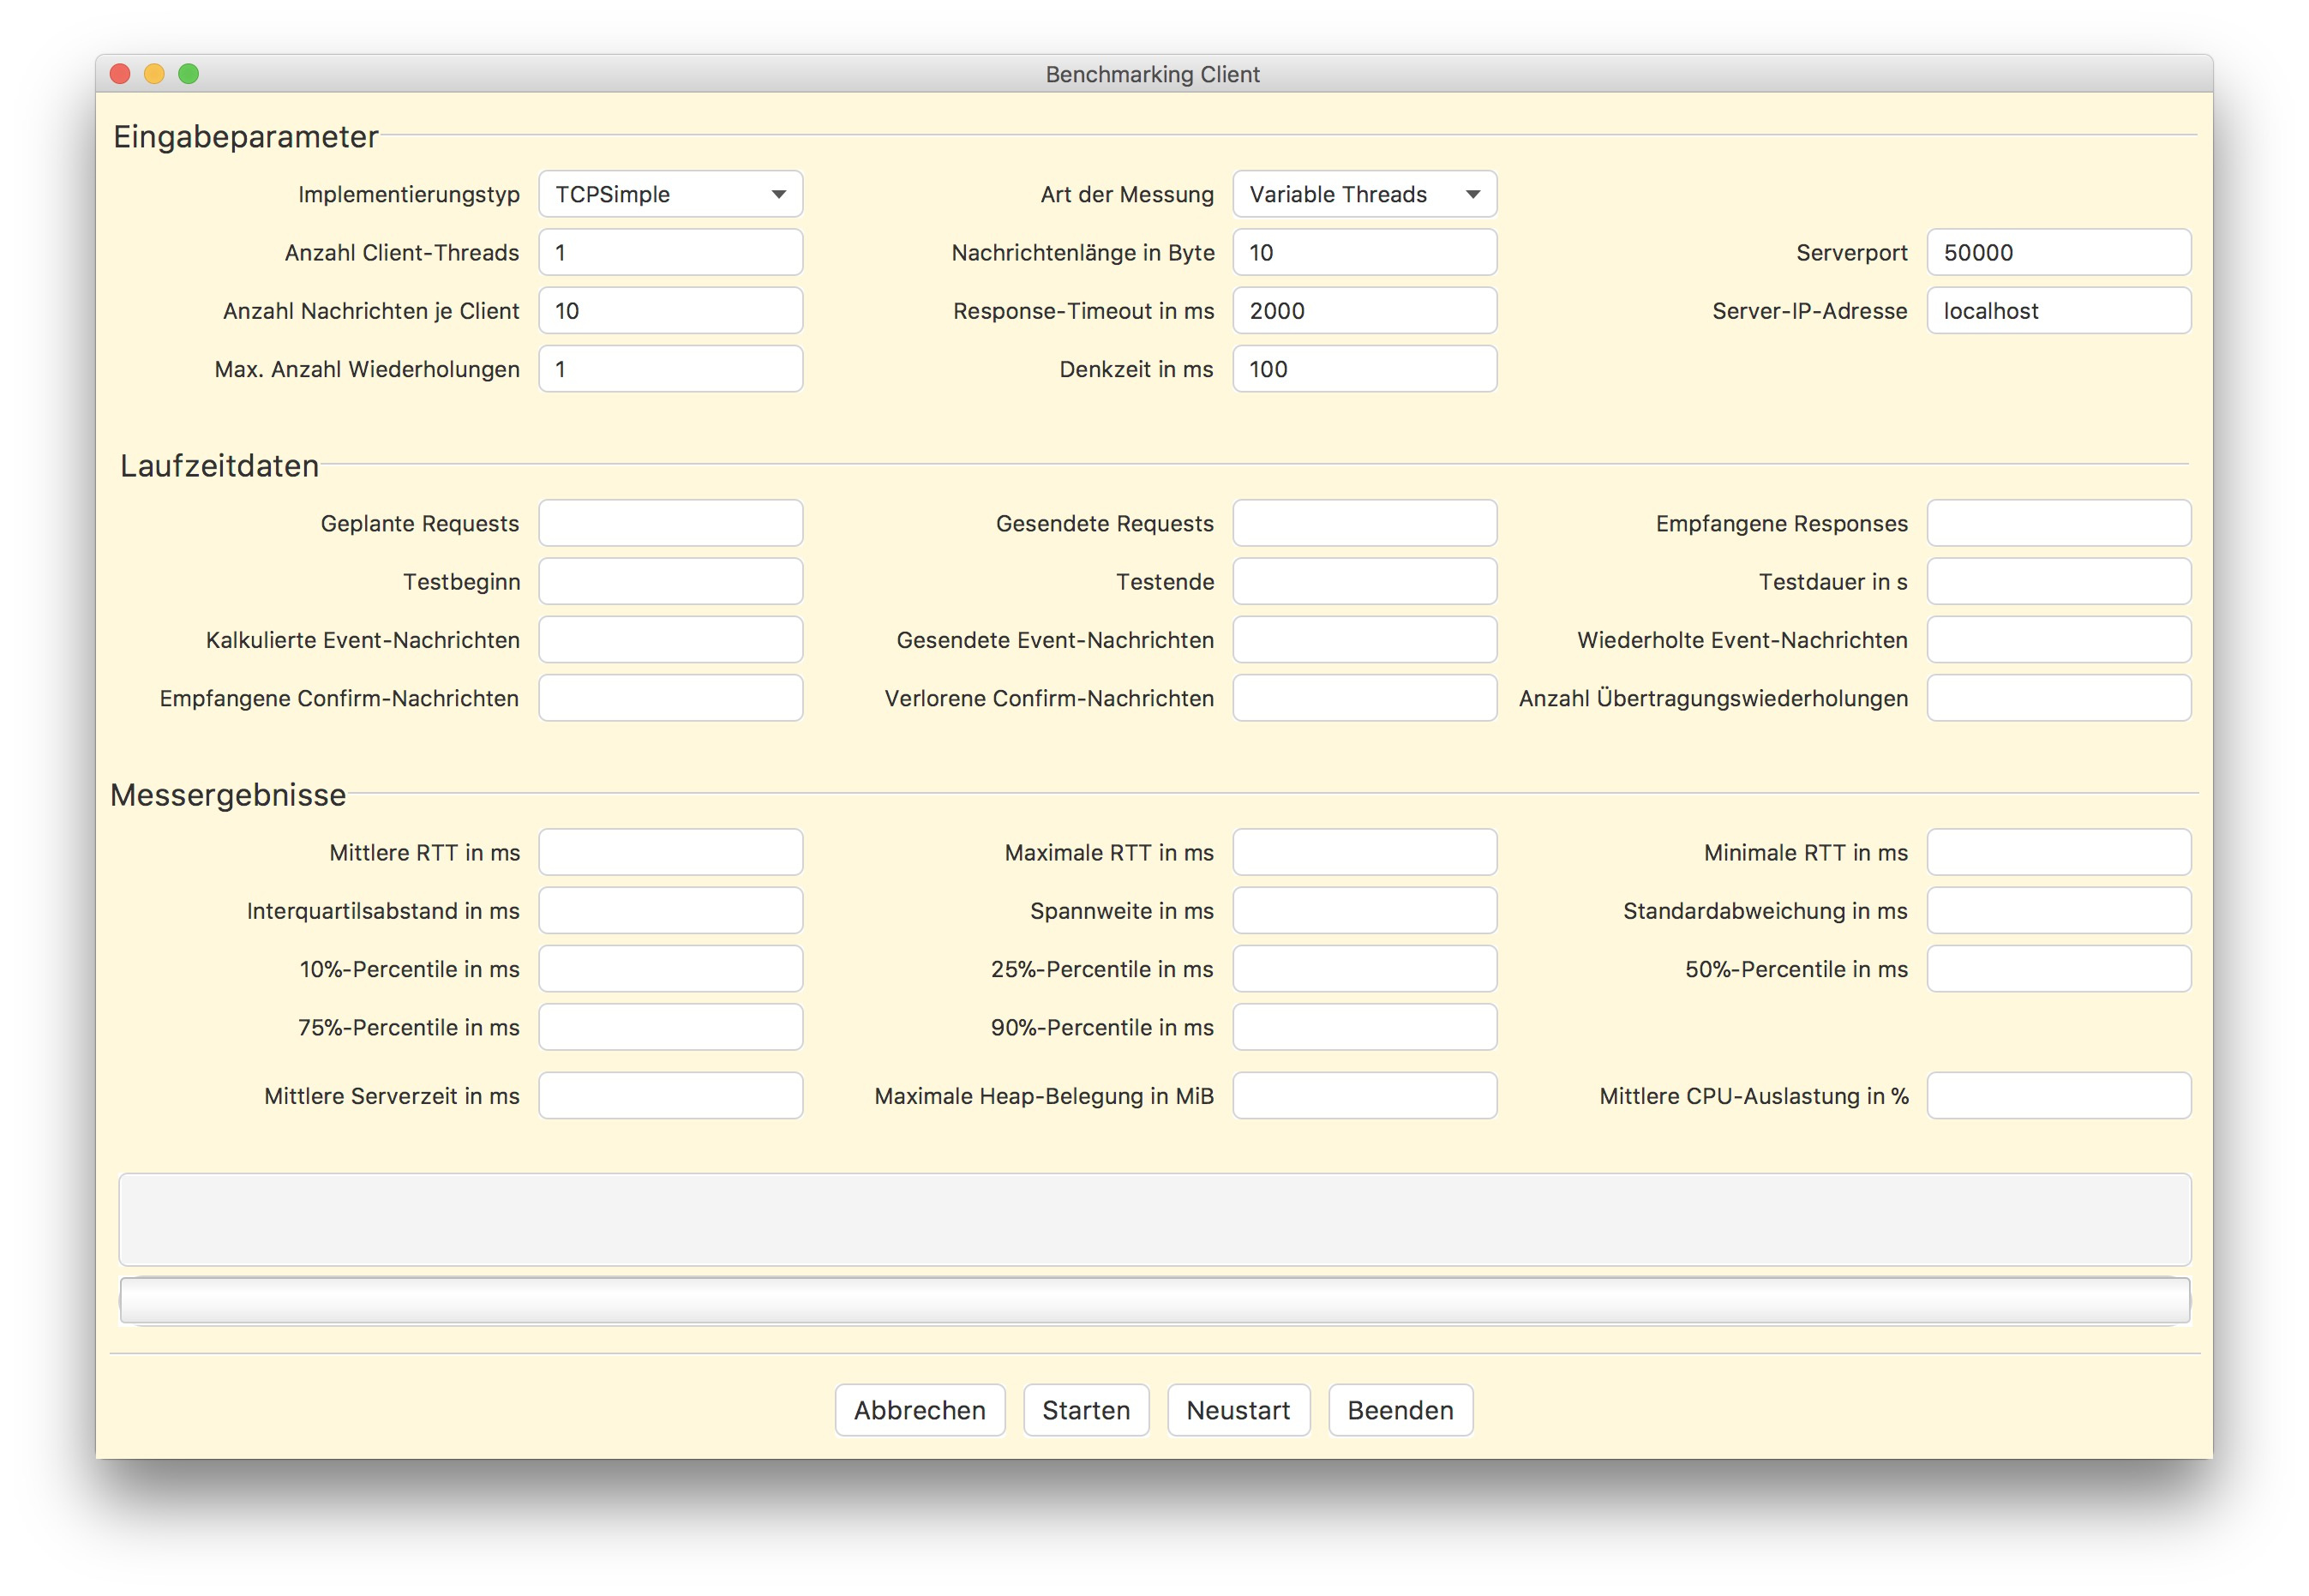
\includegraphics[scale=0.17]{img/benchClientUI.jpg}
		\caption[]{Benutzeroberfläche des Benchmark-Clients}
		\label{fig:dakoBenchClientUI}
	\end{center}
\end{figure}

\renewcommand{\arraystretch}{1.5}
\begin{table*}[ht]
	\begin{center}
		\begin{tabular}{|l|c|c|c|c|c|c|c|c|}
			\hline
			Anzahl Clients& \cellcolor{lightgrey}\textbf{3} & \textbf{15} & \cellcolor{lightgrey}\textbf{30} & \textbf{45} &\cellcolor{lightgrey}\textbf{60} & \textbf{75} & \cellcolor{lightgrey}\textbf{90} & \textbf{99} \\ \hline
			Min. RTT & \cellcolor{lightgrey}27 & 9 &\cellcolor{lightgrey}19 & 18 & \cellcolor{lightgrey}28 & 26 & \cellcolor{lightgrey}51 & 64 \\ \hline
			Max. RTT & \cellcolor{lightgrey}154 & 1991 & \cellcolor{lightgrey}5618 & 10321 & \cellcolor{lightgrey}18260 & 25881 & \cellcolor{lightgrey}35720 & 43344\\ \hline
			Mittlere RTT & \cellcolor{lightgrey}58 & 700 & \cellcolor{lightgrey}2052 & 3838 & \cellcolor{lightgrey}6642 & 9698 & \cellcolor{lightgrey}13580 & 16264 \\ \hline
			Mittlere Serverzeit & \cellcolor{lightgrey}32 & 657 & \cellcolor{lightgrey}1975 & 3745 & \cellcolor{lightgrey}6369 & 9406 & \cellcolor{lightgrey}13354 & 15970 \\ \hline
			T$_{k}$ & \cellcolor{lightgrey}26 & 43 & \cellcolor{lightgrey}77 & 93 & \cellcolor{lightgrey}273 & 192 & \cellcolor{lightgrey}226 & 294 \\ \hline
		\end{tabular}
		\caption{Ergebnisse der WebSocket-Leistungsmessung}\label{tbl:evalWebSocket}
	\end{center}
\end{table*}
\renewcommand{\arraystretch}{1}

\renewcommand{\arraystretch}{1.5}
\begin{table*}[ht]
	\begin{center}
		\begin{tabular}{|l|c|c|c|c|c|c|c|c|}
			\hline
			Anzahl Clients& \cellcolor{lightgrey}\textbf{3} & \textbf{15} & \cellcolor{lightgrey}\textbf{30} & \textbf{45} & \cellcolor{lightgrey}\textbf{60} & \textbf{75} & \cellcolor{lightgrey}\textbf{90} & \textbf{99} \\ \hline
			Min. RTT & \cellcolor{lightgrey}4 & 7 &\cellcolor{lightgrey}13 & 21 & \cellcolor{lightgrey}20 & 28 & \cellcolor{lightgrey}26 & 28 \\ \hline
			Max. RTT& \cellcolor{lightgrey}17 & 105 & \cellcolor{lightgrey}379 & 793 & \cellcolor{lightgrey}1409 & 2460 & \cellcolor{lightgrey}2414 & 2974\\ \hline
			Mittlere RTT & \cellcolor{lightgrey}8 & 32 & \cellcolor{lightgrey}158 & 364 & \cellcolor{lightgrey}557 & 978 & \cellcolor{lightgrey}1127 & 1280 \\ \hline
			Mittlere Serverzeit& \cellcolor{lightgrey}4 & 26 & \cellcolor{lightgrey}118 & 274 & \cellcolor{lightgrey}441 & 734 & \cellcolor{lightgrey}933 & 1047 \\ \hline
			T$_{k}$& \cellcolor{lightgrey}4 & 6 & \cellcolor{lightgrey}40 & 90 & \cellcolor{lightgrey}116 & 244 & \cellcolor{lightgrey}194 & 233 \\ \hline
		\end{tabular}
		\caption{Ergebnisse der TCP-Leistungsmessung}\label{tbl:evalTCP}
	\end{center}
\end{table*}
\renewcommand{\arraystretch}{1}

\begin{landscape}
\begin{figure}[ht] 
	\begin{center}
		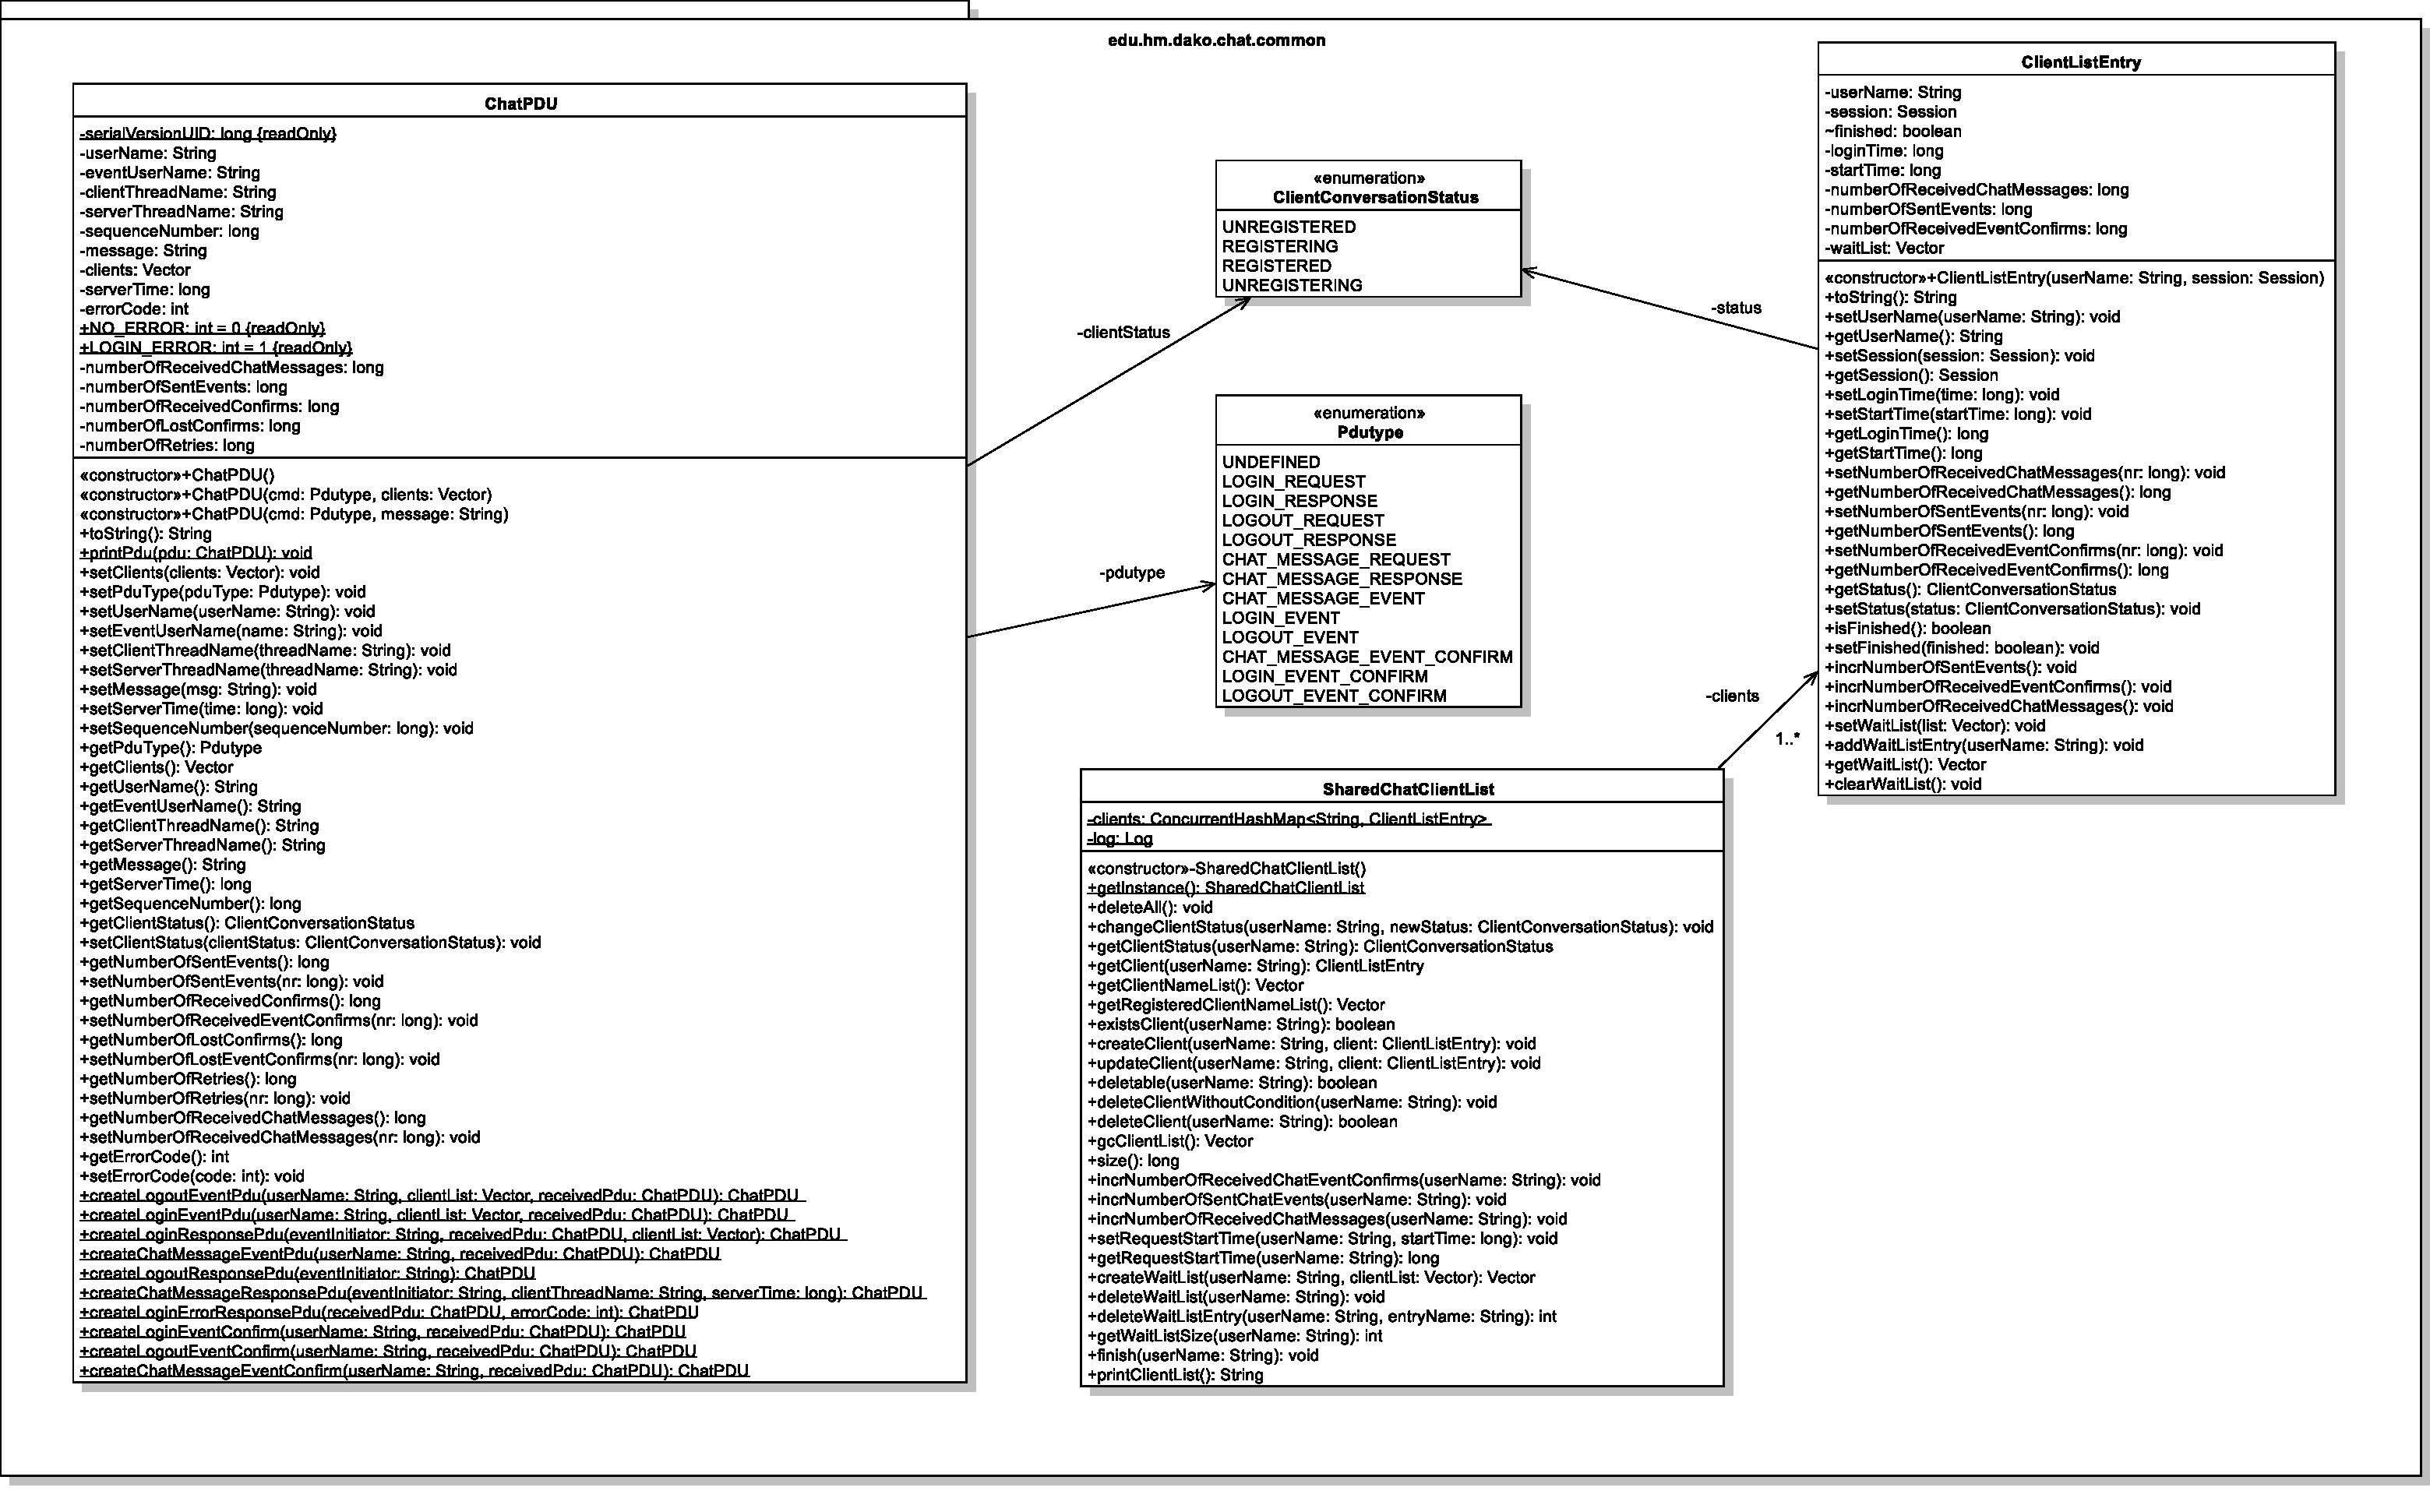
\includegraphics[scale=0.45]{img/pkgCommon.pdf}
		\caption[]{Klassendiagramm: WebSocket-Server \textit{common}-Package}
		\label{fig:kdcommon}
	\end{center}
\end{figure}
\begin{figure}[ht] 
	\begin{center}
		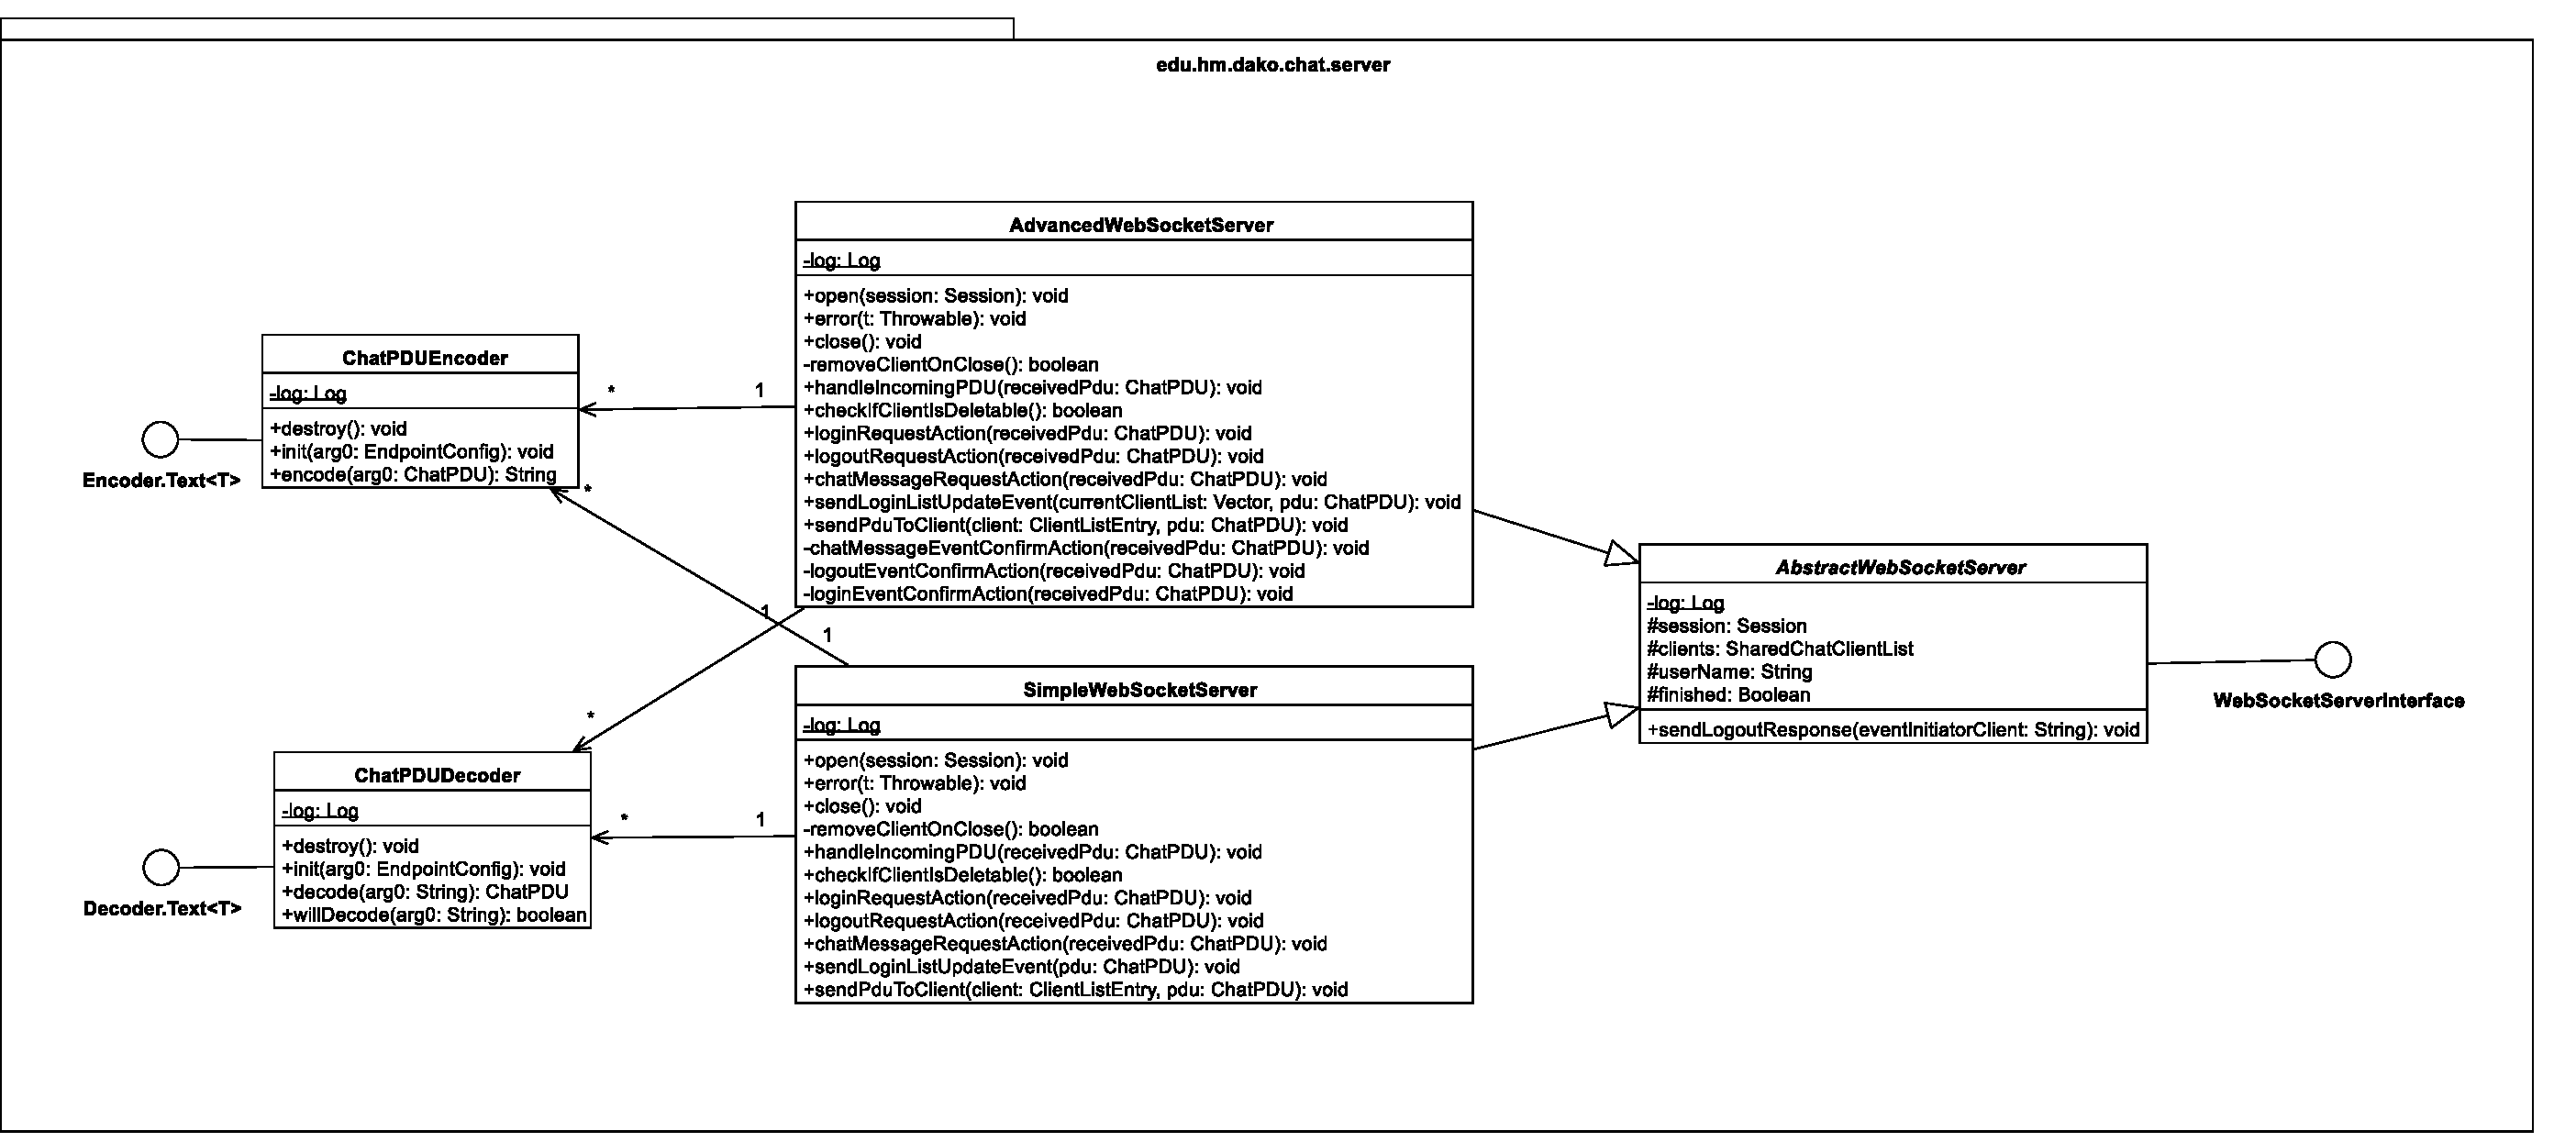
\includegraphics[scale=0.5]{img/pkgServer.pdf}
		\caption[]{Klassendiagramm: WebSocket-Server \textit{server}-Package}
		\label{fig:kdserver}
	\end{center}
\end{figure}
\begin{figure}[ht] 
	\begin{center}
		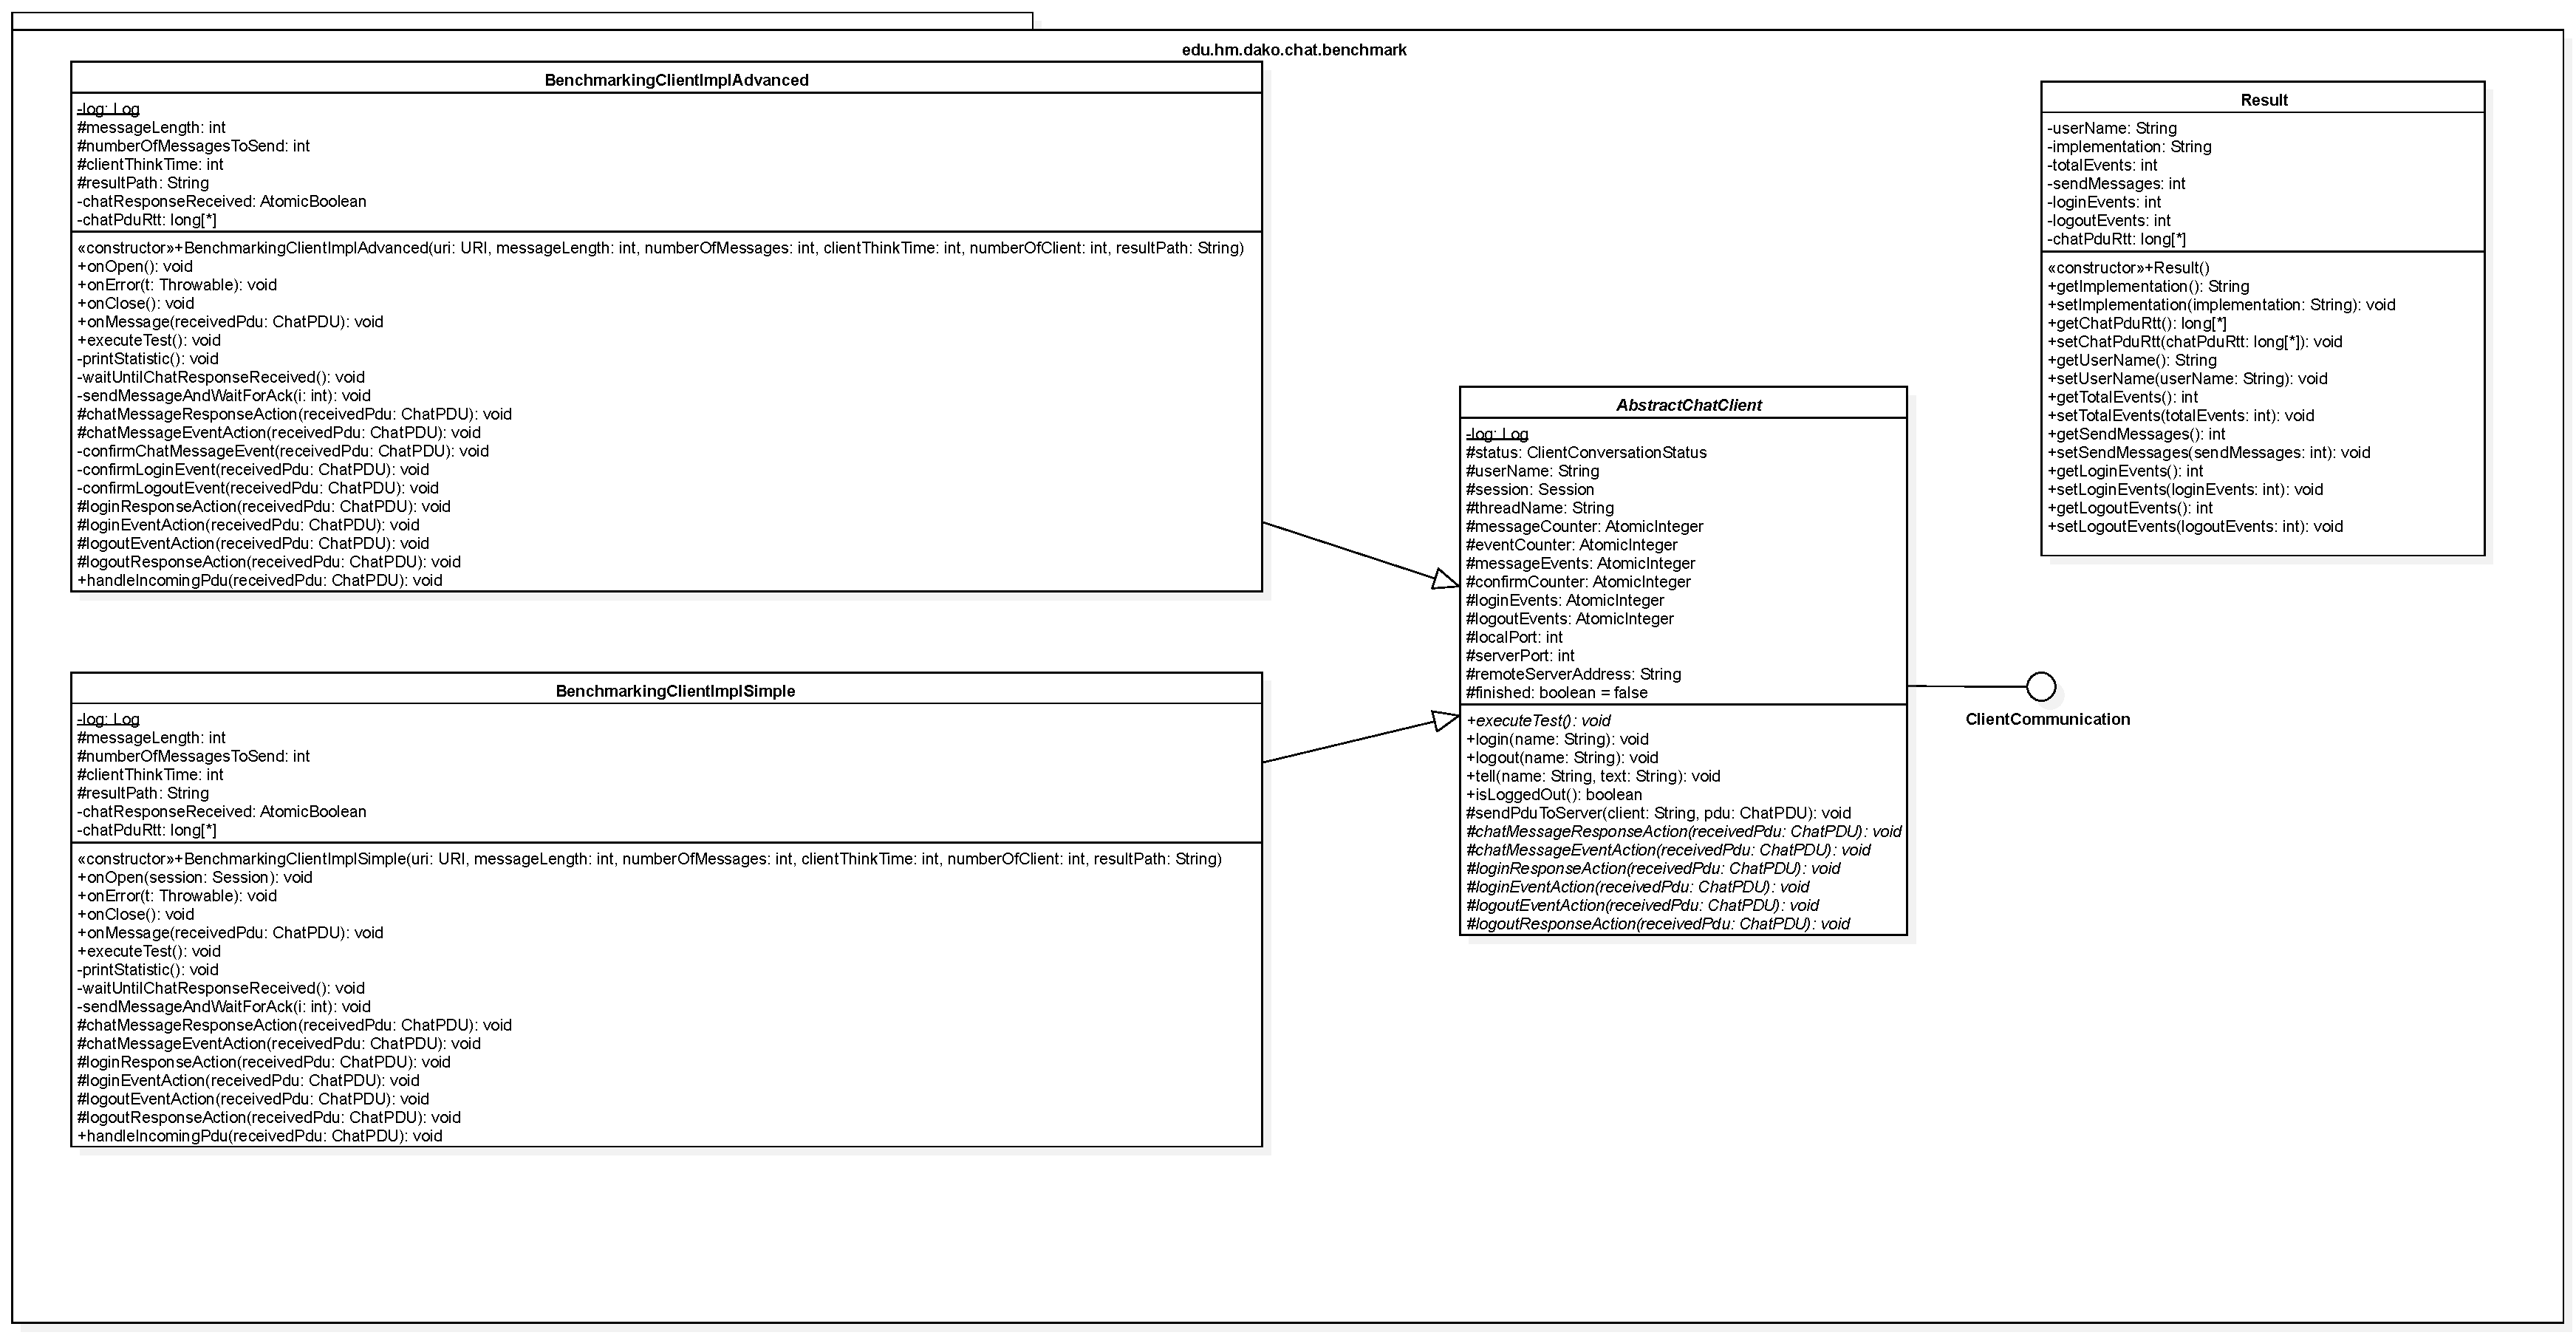
\includegraphics[scale=0.4]{img/Bench.pdf}
		\caption[]{Klassendiagramm: WebSocket-Benchmark \textit{benchmark}-Package}
		\label{fig:kdbench}
	\end{center}
\end{figure}
\begin{figure}[ht] 
	\begin{center}
		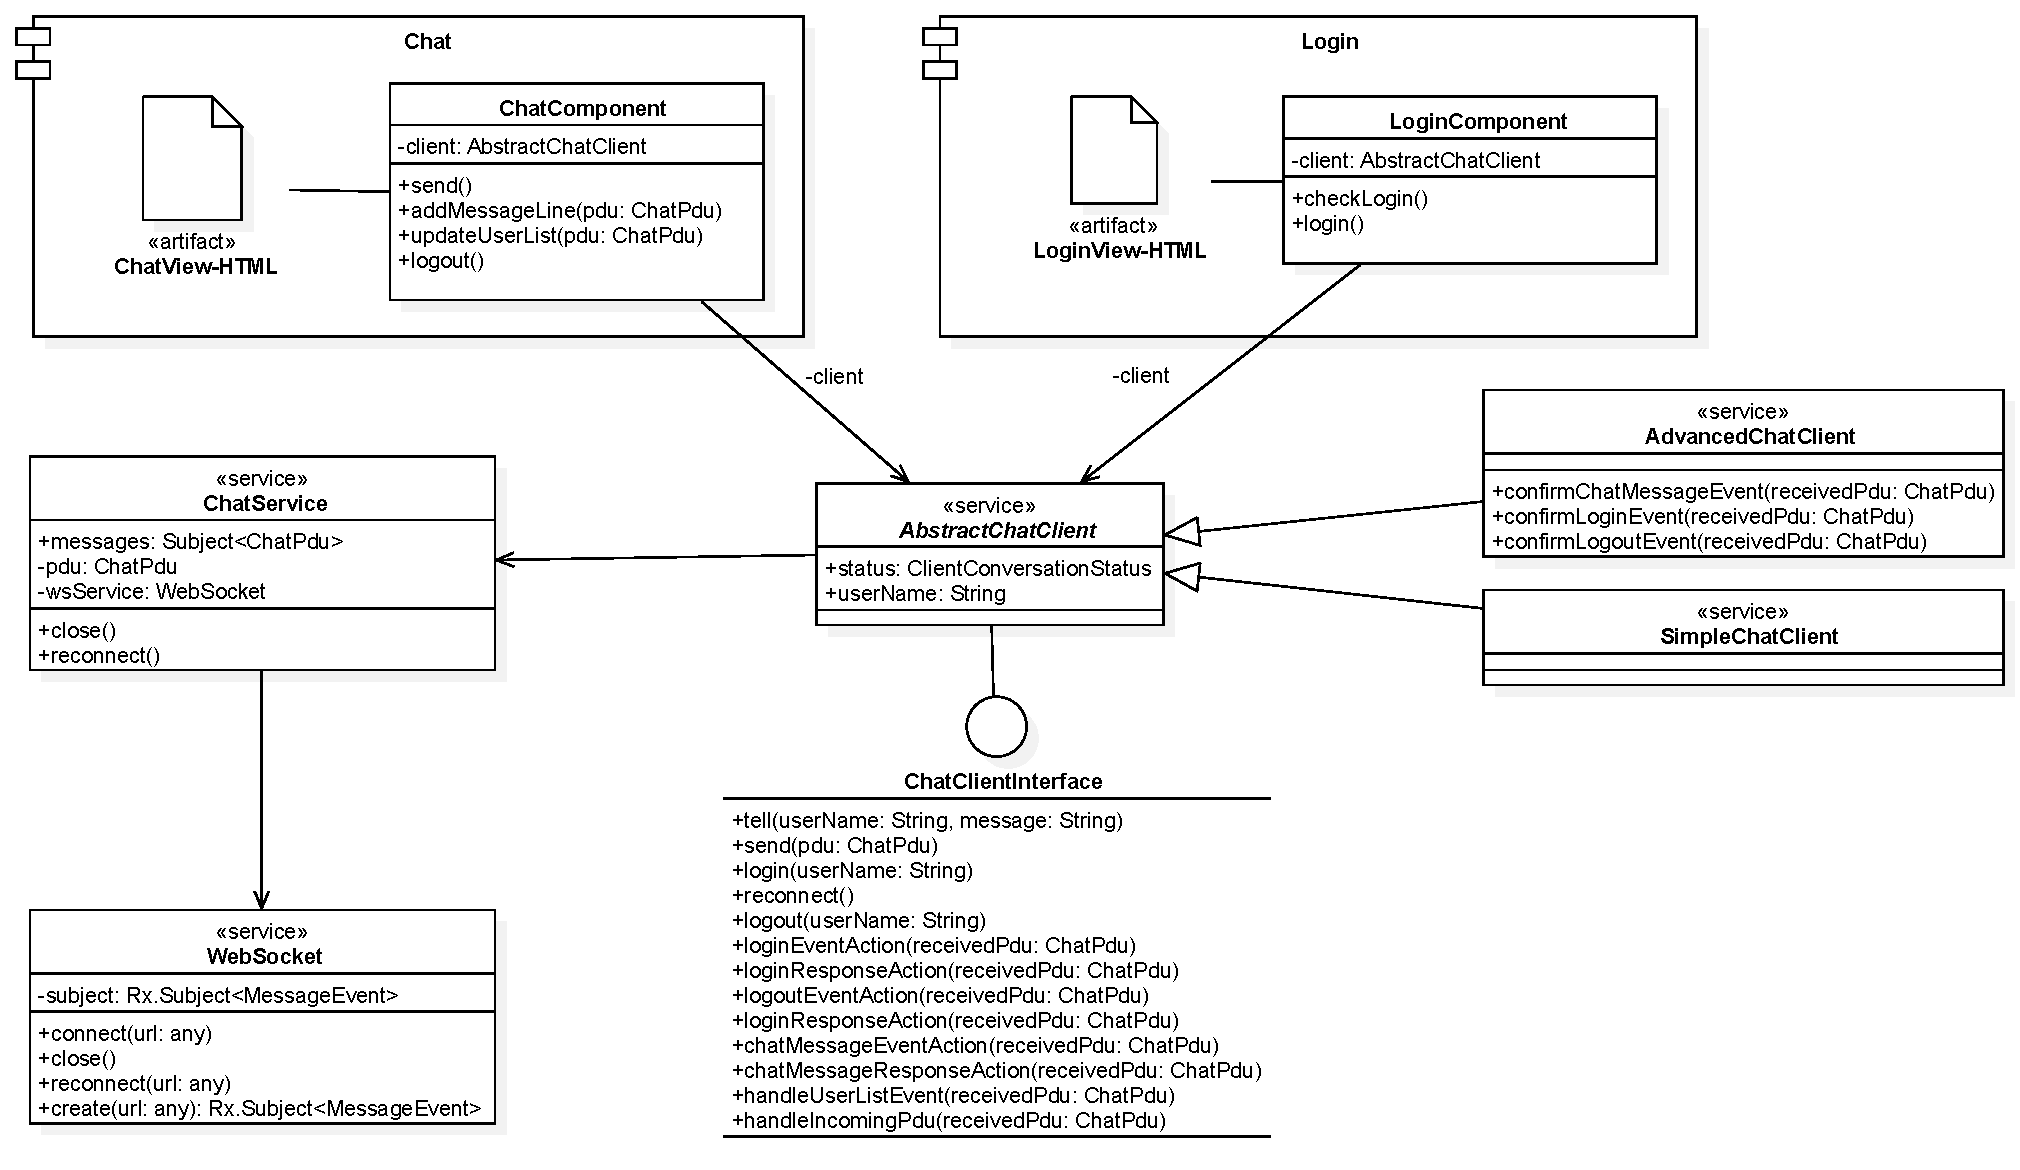
\includegraphics[scale=0.7]{img/ClientNew.pdf}
		\caption[]{Klassendiagramm: WebSocket-Client}
		\label{fig:kdClient}
	\end{center}
\end{figure}
\end{landscape}

\section*{Eidesstattliche Erklärung}

\end{document}
